\documentclass[12pt]{book}
\usepackage{graphicx,amsmath,amssymb,amsthm,geometry,caption,subcaption,booktabs,hyperref,bm,tikz} 
\graphicspath{{images/}}
\geometry{a4paper, margin=1.2in}
\usepackage{indentfirst}
\usepackage[most]{tcolorbox}
\usetikzlibrary{positioning}
\hypersetup{
	colorlinks = true,
	linkcolor  = blue,
	citecolor  = magenta,
	urlcolor   = teal
}

\usepackage{fancyhdr}
\pagestyle{fancy}
\fancyhead{}
\fancyfoot{}
\lhead{\textit{STATS 601 Lecture Notes}}
\rhead{\parbox[t]{0.5\textwidth}{\raggedright \textit{\leftmark}}}
\cfoot{\thepage}
\usetikzlibrary{shapes.geometric, positioning}
\newtheorem{theorem}{Theorem}[chapter]
\newtheorem{lemma}[theorem]{Lemma}
\theoremstyle{definition}
\newtheorem{definition}[theorem]{Definition}
\theoremstyle{remark}
\newtheorem{remark}[theorem]{Remark}

\newcommand{\R}{\mathbb{R}}
\newcommand{\E}{E}
\renewcommand{\contentsname}{CONTENT}

\usetikzlibrary{shapes.geometric, arrows.meta, positioning}

\tikzstyle{startstop} = [rectangle, rounded corners, minimum width=3cm, minimum height=1cm,text centered, draw=black, fill=gray!20]
\tikzstyle{process} = [rectangle, minimum width=3.5cm, minimum height=1cm, text centered, draw=black, fill=blue!15]
\tikzstyle{arrow} = [thick, ->, >=stealth]

\begin{document}
	
	\begin{titlepage}
		\vspace*{2cm}
		\begin{center}
			{\Huge \textbf{STATS 601 Lecture Notes}}\\[2em]
			{\Large \textit{STATS 601: Advanced Statistical Learning}}\\[4em]
                {\Large \textit{University of Michigan, Ann Arbor}}
		\end{center}
		\vfill
		\begin{flushright}
			\textbf{Author:} Ziheng Wei\\
			\textbf{Date:} \today
		\end{flushright}
	\end{titlepage}
	
	
	\tableofcontents
	\cleardoublepage
	
\newtcolorbox{notionbox}[1][]{
    colback=blue!10!white, 
    colframe=blue!50!black,
    title=#1,
    fonttitle=\bfseries,
    boxrule=0.8pt
}
\newtcolorbox{referencebox}{
    colback=green!10,
    colframe=green!50!black,
    title=\textbf{References},
    fonttitle=\bfseries,
    boxrule=1pt,
    rounded corners
}


\chapter*{Before You Read}
These notes are for \textit{STATS 601: Advanced Statistical Learning} at the University of Michigan in the Winter 2025 semester, taught by Professor \href{http://www.keanmingtan.com/}{Kean Ming Tan} and GSI \href{https://kihyukh.github.io/}{Kihyuk Hong}. The author is Ziheng Wei, a first-year Master of Applied Statistics student at UMich. \\

STATS 601 is a PhD-level course covering a broad array of statistical learning methods, with a particular focus on dimension reduction, classification, and clustering methods. Unlike other machine learning courses at UMich, such as STATS 503, EECS 545, EECS 553, and SI 670, this course places a strong emphasis on theory. For example, in the final exam you might spend more than half an hour deriving an EM-algorithm problem by hand. If you are primarily interested in machine-learning programming, you may prefer one of the four courses listed above. \\

STATS 601 is solid, especially for some master’s and undergraduate students who must invest significant effort to earn a good grade. My notes include both lecture material and Ki’s lab sessions. I hope they will help any student (even just one) taking this course, as well as statistical enthusiasts pursuing theoretical machine learning, to master the content more effectively. \\

Due to my own limitations, these notes may not always explain concepts as clearly as a textbook and may contain errors. If you find any mistakes or have suggestions for improvement, feel free to contact me at \texttt{zihwei@umich.edu}.\\

\vfill
\begin{flushright}
\textbf{Ziheng Wei}\\
Apr 28, 2025\\
(the day before the final exam)
\end{flushright}




\chapter*{Introduction}
\addcontentsline{toc}{chapter}{Introduction}
(According to the syllabus)
\section{Course Description}
This is an advanced introduction to statistical learning methods. Topics include:
\begin{enumerate}
    \item [(1)]dimension reduction techniques, including principal component analysis, factor analysis, multidimensional scaling and manifold learning; 
    \item[(2)] conceptual framework of classification including cost functions, Bayes classifiers, overfitting and generalization; specific classification methods including logistic regression, naive Bayes, discriminant analysis, support vector machines, kernel-based methods, generalized additive models, tree-based methods, boosting, neural networks;
    \item [(3)] clustering methods including K-means, model-based clustering algorithms, mixture models, latent variable models, hierarchical models; and algorithms such as the EM algorithm, Gibbs sampling, and variational inference methods;
    \item [(4)] Additional topics that may be covered include categorical data analysis, graphical models, and deep learning.
\end{enumerate}

\section{Course Outline}

\begin{itemize}
	\item \textbf{Review of multivariate Gaussian}
		
	\item \textbf{Dimension reduction methods.}
	\begin{itemize}
		\item data-driven linear dimensionality reduction (principal component analysis)
		\item model-based linear dimensionality reduction (factor analysis)
		\item nonlinear dimension reduction: multidimensional scaling and manifold learning
	\end{itemize}
		
	\item \textbf{Classification methods.}
	\begin{itemize}
		\item model-based classification: linear classification, logistic regression
		\item data-driven classification
		\item support vector machines, generalized additive models, tree-based methods,
			boosting, neural networks
	\end{itemize}
		
	\item \textbf{Clustering methods.}
	\begin{itemize}
		\item data-driven clustering: k-means, spectral clustering
		\item model-based clustering: mixture of multivariate Gaussians
		\item Dirichlet process mixtures and multivariate extensions
	\end{itemize}
		
	\item \textbf{Selective topics}
	\begin{itemize}
		\item graphical models and hierarchical models
		\item latent variable models
	\end{itemize}
\end{itemize}

\section{Grades}
There will be bi-weekly homework assignments, a midterm exam, a final exam, and an individual project.

\section{Textbooks and References}
\begin{enumerate}
    \item \textit{The elements of statistical learning} by Hastie, Friedman, and Tibshirani (henceforth \textit{ESL});
    \item \textit{Pattern recognition and machine learning} by C. Bishop (henceforth \textit{PRML});
    \item \textit{An Introduction to Multivariate Statistical Analysis} by T.W.Anderson;
    \item \textit{Aspects of multivariate statistical theory} by R.J. Muirhead;
    \item Long Nguyen’s lecture notes;
    \item Michael Jordan’s selected book chapters on graphical models.
\end{enumerate}





\newpage
\part{DIMENSION REDUCTION}
\chapter{Multivariate Normal Distribution (MVN)}

\section{Multivariate Normal Distribution}

\subsection{Definition}
Consider a $p$-dimension random vector $Z = (Z_1, \dots, Z_p)^T$, where $Z_1,\dots, Z_p \overset{i.i.d.}{\sim} N(0,1)$. We have $EZ_i=0$, $varZ_i = 1$ and $var Z= I_p$. The PDF of Z is 
\[f(Z) = \prod_{i=1}^p f(Z_i) = \frac{1}{(2\pi)^{\frac{p}{2}}}\exp(-\frac{1}{2}\sum_{i=1}^p z_i^2) = \frac{1}{(2\pi)^{\frac{p}{2}}}\exp(-\frac{1}{2}Z^TZ),\; Z\in \R^p\]
Let $B\in\R^{p\times p}$ be any non-singular matrix and $\mu \in \R^p$ be any $p$-dimensional vector. $X=BZ+\mu \in \R^p$.\\
By Jacobi transformation, the PDF of $X$ is given by
\[f(X|\mu, \Sigma) = (2\pi)^{-\frac{p}{2}}|BB^T|^{-\frac{1}{2}}\exp[-\frac{1}{2}(x-\mu)^T(BB^T)^{-1}(X-\mu)]\]
\[ = (2\pi)^{-\frac{p}{2}}|\Sigma|^{-\frac{1}{2}}\exp[-\frac{1}{2}(x-\mu)^T\Sigma^{-1}(X-\mu)]\]
where $\Sigma = BB^T$. It's obvious that $\begin{cases}EX = E(BZ+\mu) = BE(Z)+\mu = \mu
 \\cov(X) = cov(BZ) = Bcov(Z)B^T = BB^T = \Sigma \end{cases}$.

\subsection{Properties}
\begin{enumerate}
\item $\int f(x|\mu, \Sigma) dx = 1$ (property of PDF);
\item The distribution of $X$ only depends on $\mu$ and $\Sigma$;
\item The affine transformation of a Normal distribution is Normal too:\\
$X\sim N_p(\mu, \Sigma)$. Let $A\in \R^{n\times p}, b \in \R^{n\times 1}$, then $Y = AX+b \sim N_n(A\mu+b, A\Sigma A^T)$;\\

\textcolor{blue}{
\begin{proof}[Proof sketch]
Consider $X = BZ+\mu,\; Z\sim N_p(0,I_p)$, we have $Y = ABZ + A\mu+b$.\\
Then, 
$\begin{cases}E(Y)=ABE(Z)+A\mu+b = A\mu+b\\cov(ABZ) = ABI_pB^TA^T = ABB^TA^T = A\Sigma A^T\end{cases}$.
\end{proof}
}

\item The subset of a MVN distribution is Normal too:\\
$A = (I_m,\; 0)_{m\times p} = \begin{pmatrix}  
  1 & 0 & \cdots & 0 &0&\cdots&0\\  
  0 & 1 & \cdots & 0 &0&\cdots&0\\  
  \vdots & \vdots & \ddots & \vdots &0&\cdots&0\\  
  0 & 0 & \cdots & 1&0&\cdots&0 
\end{pmatrix},\quad b = 0.$ Then $AX+b = \begin{pmatrix}
X_1 \\
\vdots \\
X_m
\end{pmatrix}\sim N_m(\mu', \Sigma')$ where $\mu' = \begin{pmatrix}
\mu_1 \\
\vdots \\
\mu_m
\end{pmatrix},\; \Sigma' = \begin{pmatrix}  
  \sigma_{11} & 0 & \cdots & 0 \\  
  0 & \sigma_{22} & \cdots & 0 \\  
  \vdots & \vdots & \ddots & \vdots \\  
  0 & 0 & \cdots & \sigma_{mm}  
\end{pmatrix} $;
\item Standardization of a MVN is also MVN:\\
$X\sim N_p(\mu, \Sigma)$, then $\Sigma^{-1/2}(X-\mu)\sim N_p(0,I_p)$;
\item If $(X_1, X_2)$ follows MVN, Then $X_1$ is independent of $X_2$ $\Leftrightarrow$ $cov(X_1, X_2) = 0$;
\item Conditional distribution of MVN:\\
If $X\sim N_p(\mu, \Sigma), \Sigma_{22}$ is positive definite, where $X = \begin{pmatrix}
X_1 \\
X_2
\end{pmatrix},\; \mu = \begin{pmatrix}
\mu_1 \\
\mu_2
\end{pmatrix},\;\Sigma = \begin{pmatrix}  
  \Sigma_{11} & \Sigma_{12} \\  
  \Sigma_{21}& \Sigma_{22} 
\end{pmatrix}$. The distribution of $X_1$ given $X_2$ is 
\[X_1|X_2 \sim N(\mu_1+\Sigma_{12}\Sigma_{22}^{-1}(X_2-\mu_2), \Sigma_{11} - \Sigma_{12}\Sigma_{22}^{-1}\Sigma_{21}).\]
\end{enumerate}




\begin{notionbox}[Note]
Let \( S \in \mathbb{R}^{n \times n} \), define
\[
S =
\begin{pmatrix}
S_{11} & S_{12} \\
S_{21} & S_{22}
\end{pmatrix}
\]
where \( S_{11} \in \mathbb{R}^{n_1 \times n_1} \), \( S_{12} \in \mathbb{R}^{n_1 \times n_2} \), \( S_{21} \in \mathbb{R}^{n_2 \times n_1} \), \( S_{22} \in \mathbb{R}^{n_2 \times n_2} \) and \( n_1 + n_2 = n \).

Consider partition
\[
\begin{pmatrix}
I_{n_1} & -S_{12} S_{22}^{-1} \\
0 & I_{n_2}
\end{pmatrix}
\begin{pmatrix}
S_{11} & S_{12} \\
S_{21} & S_{22}
\end{pmatrix}
\begin{pmatrix}
I_{n_1} & 0 \\
-S_{22}^{-1} S_{21} & I_{n_2}
\end{pmatrix}
=
\begin{pmatrix}
S_{11.2} & 0 \\
0 & S_{22}
\end{pmatrix}
\]
where
\[
S_{11.2} = S_{11} - S_{12} S_{22}^{-1} S_{21}
\]
\end{notionbox}

\begin{notionbox}[Note]
Then
\[
\begin{pmatrix}
S_{11} & S_{12} \\
S_{21} & S_{22}
\end{pmatrix}
=
\begin{pmatrix}
I_{n_1} & S_{12} S_{22}^{-1} \\
0 & I_{n_2}
\end{pmatrix}
\begin{pmatrix}
S_{11.2} & 0 \\
0 & S_{22}
\end{pmatrix}
\begin{pmatrix}
I_{n_1} & 0 \\
S_{22}^{-1} S_{21} & I_{n_2}
\end{pmatrix}
\]

Its inverse matrix is 
\[\begin{pmatrix}S_{11} & S_{12} \\
S_{21} & S_{22}\end{pmatrix}^{-1}=
\begin{pmatrix}I_{n_1} & 0 \\
-S_{22}^{-1} S_{21} & I_{n_2}\end{pmatrix}
\begin{pmatrix}S_{11.2}^{-1} & 0 \\
0 & S_{22}^{-1}\end{pmatrix}
\begin{pmatrix}I_{n_1} & -S_{12} S_{22}^{-1} \\
0 & I_{n_2}\end{pmatrix}\]

So
\[X^T S^{-1} X = (X_1 - S_{12} S_{22}^{-1} X_2)^T S_{11.2}^{-1} (X_1 - S_{12} S_{22}^{-1} X_2) + X_2^T S_{22}^{-1} X_2\]
\end{notionbox}
From the notes above, we know that 
\[(X^T-\mu) \Sigma^{-1} (X-\mu) = (X_1 -\mu_1- \Sigma_{12} \Sigma_{22}^{-1} (X_2-\mu_2))^T \Sigma_{11.2}^{-1}  (X_1 -\mu_1- \Sigma_{12} \Sigma_{22}^{-1} (X_2-\mu_2))\]\[ + (X_2-\mu_2)^T \Sigma_{22}^{-1}(X_2-\mu_2)\]
which means $f(X_1, X_2) = f(X_1|X_2)f(X_2)$.\\

A fun fact is $X_1 - \Sigma_{12} \Sigma_{22}^{-1}X_2 \perp X_2$.\\

\textcolor{blue}{
\begin{proof}[Proof sketch]
Use property 3 and 6 above. 
Define matrix \( A \) as:
\[A =\begin{pmatrix}
I_{p_1} & -\Sigma_{12} \Sigma_{22}^{-1} \\
0 & I_{p_2}\end{pmatrix}\]
Multiplying by vector:
\[AX =\begin{pmatrix}
X_1 - \Sigma_{12} \Sigma_{22}^{-1} X_2 \\
X_2\end{pmatrix}\]
Since \( X \sim N(\mu, \Sigma) \), we have:
\[AX \sim N(A\mu, A \Sigma A^T)\]
which follows:
\[\mathcal{N}_p \left(\begin{pmatrix}
\mu_1 - \Sigma_{12} \Sigma_{22}^{-1} \mu_2 \\
\mu_2\end{pmatrix},\begin{pmatrix}\Sigma_{11.2} & 0 \\
0 & \Sigma_{22}\end{pmatrix}\right)\]
The covariance is 0. Thus, it follows that they are independent.\\
So the conditional distribution:
\[X_1 - \Sigma_{12} \Sigma_{22}^{-1} X_2 \mid X_2 \sim N(\mu_1 - \Sigma_{12} \Sigma_{22}^{-1} \mu_2, \Sigma_{11.2})\]
Therefore:
\[X_1 \mid X_2 \sim N(\mu_1 + \Sigma_{12} \Sigma_{22}^{-1} (X_2 - \mu_2), \Sigma_{11.2})\]
\end{proof}
}

Expectation of \( X_1 \) given \( X_2 \) can be regarded as the regression mean function of $X_1$ on $X_2$. $\Sigma_{12} \Sigma_{22}^{-1}$ is the regression coefficient.
\textcolor{blue}{
\begin{proof}[Proof sketch]
Recall OLS: $X_1 \sim X_2$. The estimated regression coefficient is $\hat{B} = (X_2^TX_2)^{-1}X_2^TX_1 = \Sigma_{22}^{-1}\Sigma_{12}$.
\end{proof}
}

\subsection{Canonical representation of MVN}
The canoncial representation of MVN $X\sim N_p(\mu, \Sigma)$ is: 
\[f(X|\mu,\Sigma) = \exp\{a+\frac{1}{2}X^T\Theta X\}\]
where \[\left\{\begin{matrix}
a = -\frac{1}{2}[p\log(2\pi)-\log|\Theta|+\eta^T\Theta^{-1}\eta] \\
\Theta = \Sigma^{-1} \\
\eta = \Theta \mu
\end{matrix}\right.\]
\\
One application: \textbf{Gaussian Graphical Model} (GGM).\\
We will discuss about it in the next section.


\begin{referencebox}
\begin{enumerate}
    \item Chapter 17. \textit{ESL}.
    \item Meinshausen, N., \& Bühlmann, P. (2006). High-dimensional graphs and variable selection with the lasso.
    \item Speed, T.P. and Kiiveri, H.T., 1986. Gaussian Markov distributions over finite graphs. \textit{The Annals of Statistics}, pp.138-150.
    \item Friedman, J., Hastie, T. and Tibshirani, R., 2008. Sparse inverse covariance estimation with the graphical lasso. \textit{Biostatistics}, 9(3), pp.432-441.
\end{enumerate}
\end{referencebox}


\subsection{Maximum Likelihood Estimation of MVN}
Let \( X_1, \dots, X_n \overset{i.i.d.}{\sim} N_p(\mu, \Sigma) \quad (n \gg p) \).\\

\textbf{Theorem}: The MLEs for \( \mu \) and \( \Sigma \) are:

\[\begin{cases}
\hat{\mu} = \bar{X}\\
\hat{\Sigma} = \frac{1}{n} \sum_{i=1}^{n} (X_i - \bar{X}) (X_i - \bar{X})^T\end{cases}
\]

\textcolor{blue}{
\begin{proof}
\[
f(X \mid \mu, \Sigma) = \frac{1}{(2\pi)^{p/2} |\Sigma|^{1/2}} \exp \left\{ -\frac{1}{2} (X - \mu)^T \Sigma^{-1} (X - \mu) \right\}
\]
So the likelihood function is:
\[L(\mu, \Sigma) = \prod_{i=1}^{n} f(X_i \mid \mu, \Sigma)\]
\[= (2\pi)^{-np/2} |\Sigma|^{-n/2} \exp \left\{ -\frac{1}{2} \sum_{i=1}^{n} (X_i - \mu)^T \Sigma^{-1} (X_i - \mu) \right\}\]
\[= (2\pi)^{-np/2} |\Sigma|^{-n/2} \exp \left\{ -\frac{1}{2} tr[ \Sigma^{-1}\sum_{i=1}^{n} (X_i - \mu)(X_i - \mu)^T] \right\}\]
The log likelihood function is:
\[\log L = c + \frac{n}{2} \log |\Sigma^{-1}| - \frac{1}{2} tr (\Sigma^{-1} A)\]
where $A = \sum_{i=1}^{n} (X_i - \mu) (X_i - \mu)^T$.\\
\\
To find MLE of \( \mu, \Sigma \):\\
First compute the derivative with respect to (henceforth \textit{"w.r.t."}) $\mu$:
\[\frac{\partial \log L}{\partial \mu} = 0
\Rightarrow \frac{\partial \log L}{\partial \mu} = \sum_{i=1}^{n} (X_i - \mu) ^T \Sigma^{-1} = 0
\Rightarrow \frac{1}{n} \sum_{i=1}^{n} (X_i - \hat{\mu}) = 0\]
So\[\hat{\mu} = \bar{X}\]
\begin{notionbox}[Note]
\begin{itemize}
    \item $\frac{\partial \log |A|}{\partial A} = A^{-1}$;
    \item $\frac{\partial tr(AB)}{\partial A} = B^T$;
    \item $\frac{\partial tr(A B A^T)}{\partial A} = A(B + B^T)$;
    \item $\frac{\partial tr(BA^TCA)}{\partial A} = 2 CAB$ if $B,C$ are symmetric.
\end{itemize}
\end{notionbox}
Calculate the derivative w.r.t. \(\mathbf{\Sigma^{-1}}\):
\[\frac{\partial \log L}{\partial \Sigma^{-1}} = \frac{n}{2} \Sigma - \frac{1}{2} A^T = 0\]
\[\Rightarrow \hat{\Sigma} = \frac{1}{n} \hat{A} = \frac{1}{n}\sum_{i=1}^{n} (X_i - \bar{X}) (X_i - \bar{X})^T\]
\end{proof}
}
\newpage
\section{Convex Optimization}
\subsection{Norm}
\begin{enumerate}
    \item [\textbf{A.}] \textbf{Vector Norm} $\left \| \cdot  \right \| _{r} $:\\
    $\forall\vec{x},\vec{y}\in\mathbb{R}^{n}$ , vector norm of $\mathbb{R}^{n} (\left \| \cdot  \right \|)$ satisfies:\\
(1) $\left \| \vec{x}  \right \|\ge0$, $\left \| \vec{x}  \right \|=0\Leftrightarrow \vec{x}=0$; \\
(2) $\forall\lambda\in\mathbb{R}$ , $\left \| \lambda\vec{x} \right \| =\left | \lambda  \right | \left \| \vec{x} \right \|$; \\
(3) triangle inequality: $\left \| \vec{x}+\vec{y} \right \| \le \left \| \vec{x} \right \| + \left \| \vec{y} \right \|$.\\
\begin{notionbox}[Note]
frequently used vector norms:\\
\textbf{L1 Norm}: $\left \| \vec{x} \right \|_{1} =\sum_{i=1}^{n}\left | x_{i}  \right |$;

\textbf{L2 Norm (Euclidean Norm)}: $\left \| \vec{x} \right \|_{2} =\sqrt{\vec{x}^{T}\vec{x}} =\sqrt{\sum_{i=1}^{n}\left | x_{i}  \right | ^{2} }$;

\textbf{L-infinity Norm (Chebyshev Norm)}: $\left \| \vec{x} \right \|_{\infty} =\underset{1\le i\le n}{\max}\left | x_{i} \right |$.
\end{notionbox}

\item [\textbf{B.}] \textbf{Matrix Norm} $\left \| \cdot \right \| _{M}$:\\\label{sec:matrix norm origin}
$\forall\mathrm{A}$, $\mathrm{B}\in\mathbb{R}^{n\times n}$, matrix norm of $\mathbb{R}^{n\times n}$($\left \| \cdot \right \|$) satisfies:\\
(1) $\left \|\mathrm{A}\right \|\ge0$, $\left \|\mathrm{A}\right \|=0\Leftrightarrow \mathrm{A}=0$;\\
(2) $\forall\lambda\in\mathbb{R}$, $\left \| \lambda\mathrm{A} \right \| =\left | \lambda  \right | \left \| \mathrm{A} \right \|$;\\
(3) triangle inequality: $\left \| \mathrm{A+B}\right \| \le \left \| \mathrm{A} \right \| + \left \|\mathrm{B}\right \|$.\\

if it satisfies (4) $\left \| \mathrm{A\cdot B}\right \| \le \left \| \mathrm{A} \right \| \cdot \left \|\mathrm{B}\right \|$ , then we call it compatible matrix norm or modulus.
\begin{notionbox}[Note]\begin{itemize}
    \item \textbf{Frobenius-Norm (F-Norm)}: $\left \| \mathrm{A} \right \| _{F} = \sqrt{<\mathrm{A},\mathrm{A}>} = \sqrt{tr(\mathrm{A^T}\mathrm{A})} = \sqrt{\sum_{i=1}^{m}\sum_{j=1}^{n} a_{ij}^{2}}$. Often used to measure the error of matrices (L2 loss);
    \item \textbf{1-Norm (Column Sum Norm)}: $\left \| \mathrm {A}    \right \| _{1} = \underset{\left \| \vec{x} \right \|=1 }{\max}\left \| \mathrm {A}\vec{x}\right \|_{1}=\underset{1\le j\le n}{\max} \sum_{i=1}^{m}\left | a_{ij} \right |$,  the maximum absolute column sum of the matrix;
    \item \textbf{2-Norm (Spectral Norm)}: $\left \| \mathrm {A}\right \| _{2}=\underset{\left \| \vec{x} \right \| =1}{\max} \left \| \mathrm {A}  \vec{x}  \right \|_{2} =\max\sqrt{\rho (\mathrm{A^{T}A})}$, the square root of the maximum eigenvalue of the matrix multiplied by its conjugate transpose;
    \item \textbf{Infinity Norm (Row Sum Norm)}: $\left \| \mathrm {A}    \right \| _{\infty, \infty} = \underset{\left \| \vec{x} \right \|=1 }{\max}\left \| \mathrm {A}\vec{x}\right \|_{\infty}=\underset{1\le i\le m}{\max} \sum_{j=1}^{n}\left | a_{ij} \right |$, the maximum absolute row sum of the matrix;
    \item \textbf{nuclear norm}:$ \|B\|_*= \sum_{i=1}^q \sigma_i(B)$, the sum of all the singular values of B. Often used to control the rank of a matrix in sparse low-rank modeling;
    \item $\|B\|_{1,2}: =\sum_{i=1}^q \|B_i\|_2$ row sum of L2-norm of each row vectors;
    \item $\|X\|_{1,1} = \sum_{j,k}|X_{jk}|$ the sum of the absolute values for all elements in $X$;
    \item $\|X\|_{2,0} = \sum_{i=1}^n \mathbb{I}_{\{\|X_{i,:}\|_2 \neq 0\}}$ is the number of non-zero rows in $X$;
    \item $ \|diag(X)\|_0 = \sum_{i=1}^n \mathbb{I}_{\{X_{ii} \neq 0\}}$ is the number of non-zeros diagonal entries in $X$.
\end{itemize}
\end{notionbox}
\end{enumerate}

\subsection{Convex optimization problem}
\[\text{minimize} \quad f(\textbf{\textit{x}})\]
\[\text{subject to} \quad \begin{matrix}g_i(\textbf{\textit{x}})\le 0, \quad i=1,\dots,m
 \\h_i(\textbf{\textit{x}})= 0, \quad i=1,\dots,p
\end{matrix}\]
where the optimization variable $\textbf{\textit{x}} \in \R^n$ and
\begin{itemize}
    \item $f : \mathbb{R}^n \to \mathbb{R}$ is convex and differentiable.
    \item $g_i : \mathbb{R}^n \to \mathbb{R}$ are convex and differentiable.
    \item $h_i : \mathbb{R}^n \to \mathbb{R}$ are affine and differentiable.
\end{itemize}

\paragraph{1. Lagrangian function:}
\[
\mathcal{L}(\textbf{\textit{x}}; \mu, \lambda):= f(\textbf{\textit{x}})+ \sum_{i=1}^m \mu_i\,g_i(\textbf{\textit{x}})+ \sum_{j=1}^p \lambda_j\,h_j(\textbf{\textit{x}})\]

\paragraph{2. KKT conditions}
\begin{itemize}
    \item $g_i(\mathbf{x}) \leq 0, \quad i = 1, \dots, m.$ \hfill (feasibility)
    \item $h_i(\mathbf{x}) = 0, \quad i = 1, \dots, p.$ \hfill (feasibility)
    \item $\mu_i \geq 0, \quad i = 1, \dots, m.$
    \item $\lambda_i g_i(\mathbf{x}) = 0, \quad i = 1, \dots, m.$
    \item $\nabla_{\mathbf{x}} \mathcal{L}(\mathbf{x}; \mu, \lambda) = 0.$
\end{itemize}

\paragraph{3. Slater's condition}

There exists $\mathbf{x}$ such that $g_i(\mathbf{x}) < 0, \quad i = 1, \dots, m$ and $h_i(\mathbf{x}) = 0, \quad i = 1, \dots, p$.\\
\\
\\
\textbf{Theorem}:
If Slater’s condition holds, then KKT conditions $\iff$ optimality.\\
\\
Note that in many optimization problems, not necessarily convex, optimality implies KKT conditions.
\\
\\
\\
\subsection{Example: Projection onto a vector space}
The projection of $y\in\R^n$ onto a subspace $\mathcal{S} \subseteq \R^n$ is 
\[\text{Proj}_{\mathcal{S}}(y) = \underset{x\in \mathcal{S}}{\arg \min}\|x-y\|_2\]
Let $X\in\R^{n\times p}$ be a full rank matrix with $n\ge p$. Show that projection of $y$ onto the column space of $X$ is $X(X^TX)^{-1}y$.

\textcolor{blue}{
\begin{proof}
    \[X\in \mathcal{C}(X) \Leftrightarrow X = XZ\quad \text{for some Z}\]
    \[\therefore \min_{X \in C(X)} \|X - b\|_2^2 = \min_{Z \in \mathbb{R}^n} \|XZ - y\|_2^2.\]
    The Lagrangian function 
    \[L = \|XZ - y\|_2^2 = (XZ - y)^T (XZ - y)\]\[= Z^T X^T XZ - 2 y^T XZ + y^T y\]
    Calculate the partial derivative:
    \[\frac{\partial L}{\partial z} = 2X^T XZ - 2X^T y = 0\]
    If $X^T X$ is inverse, then 
    \[Z^* = (X^T X)^{-1} X^T y\]
    So the projection of $y$ on $\mathcal{C}(X)$ is denoted by
    \[\text{Proj}_{\mathcal{C}(X)}(y) = Xz^* = X (X^T X)^{-1} X^T y.\]
\end{proof}
}



\subsection{Example: Eigenvalue Decomposition}
\begin{notionbox}[Note]
    \textbf{Eigenvalue Decomposition} \\A symmetric matrix \( A \in \mathbb{R}^{n \times n} \) can be expressed as
\[A = U \Lambda U^T\]
where \( U  = (\mathbf{u}_1, \dots, \mathbf{u}_n)\) is an orthogonal matrix and \( \Lambda = \text{diag}(\lambda_1, \dots, \lambda_n) \) is diagonal.
\( \mathbf{u}_i \) is an eigenvector of \( A \) with eigenvalue \( \lambda_i \).
\end{notionbox}

Let $A$ be a symmetric matrix with $A = U\Lambda U^T$.
\begin{itemize}
    \item Verify that $tr(A) = \sum_{i=1}^n \lambda_i$.
    \item Find $\underset{x\in\R^n}{\max}x^TAx$ s.t. $\|x\| = 1$ where $A$ is symmetric.
\end{itemize}

\textcolor{blue}{
\begin{proof}[Proof sketch]The proof is as follows.\\
\begin{itemize}
    \item $tr(A) = tr(U\Lambda U^T) = tr(U^T U\Lambda) = tr(\Lambda)$.
    \item The Lagrangian function:
    \[L = x^TAx+\mu(1-x^Tx)\]
    \[\frac{\partial L}{\partial x} = 2Ax - 2\mu x = 0\]
    Therefore $Ax = \mu x$, which implies $(X,\mu)$ are eigenvectors and the corresponding eigenvalues of $A$.
\end{itemize}
\end{proof}
}







\newpage
\section{Applications of MVN (I): Gaussian Graphical Models}
\subsection{Conditional Independence}
Let $X_1, \dots, X_n \overset{i.i.d.}{\sim} N(\mu, \Sigma)$, $X = (X_1, \dots, X_n)$. The MLE for mean $\mu \in \R^d$ and covariance $\Sigma \in \R^{d\times d}$ are 
\[\hat{\mu} = \frac{1}{n}\sum_{i=1}^n X_i = \frac{1}{n} X^T \mathbf{1}_n\]
\[\hat{\Sigma} = \frac{1}{n}(X - \mathbf{1}_n\hat{\mu}^T)^T(X - \mathbf{1}_n\hat{\mu}^T)\]
Let $\Theta = \Sigma^{-1}$ denote the precision matrix. We have:
\begin{itemize}
    \item $\Sigma_{ij} = 0 \Leftrightarrow X_i \perp X_j$;
    \item $\Theta_{ij} = 0 \Leftrightarrow X_i \perp X_j | X_{-(i,j)}$.
\end{itemize}
We estimate the dependence structure by estimating $\Sigma$ and $\Theta$.

\subsection{Graphical Models}
Consider a collection $X = X_1, \dots, X_d$ of random variables. We want to represent dependence structure within $X$.\\
For an undirected graphical model, it has three key components:
\begin{itemize}
    \item A graph \( G = (V, E) \).
    \item Nodes (vertices) \( V = \{X_1, \dots, X_d\} \).
    \item Edges \( E \subseteq V \times V \).
\end{itemize}

\subsection{Pairwise Markov Property}
The Pairwise Markov Property of an undirected model:
\[
(i, j) \notin E \quad \iff \quad X_i \perp X_j \mid X_{-(i,j)}.
\]

Pairwise Markov Property \(\iff\) Global Markov Property $(A \perp B \mid C)$
for subsets of nodes \( A \) and \( B \) separated by \( C \).\\

\( C \) separates \( A \) and \( B \) if no path between \( A \) and \( B \) when \( C \) is removed from the graph.\\


\paragraph{}
\begin{center}
\begin{tikzpicture}
    % Nodes
    \node[draw, circle] (X2) {\(X_2\)};
    \node[draw, circle, below left=1.5cm and 1.2cm of X2] (X1) {\(X_1\)};
    \node[draw, circle, below right=1.5cm and 1.2cm of X2] (X3) {\(X_3\)};

    % Edges
    \draw (X1) -- (X2);
    \draw (X2) -- (X3);
\end{tikzpicture}
\end{center}

Set of nodes: $V = \{X_1, X_2, X_3\}$; Set of edges: $E = \{(X_1, X_2), (X_2, X_3)\}$.\\
\\
Here we have $X_1 \perp X_3 | X_2$.\\
\\
\textbf{Examples 1.3.1}\\
\\
\\
\begin{tikzpicture}
    % First graph (Complete Graph K4)
    \node[draw, circle, fill=blue!20] (A1) {A};
    \node[draw, circle, fill=blue!20, right=0.8cm of A1] (B1) {B};
    \node[draw, circle, fill=blue!20, below=0.8cm of A1] (D1) {D};
    \node[draw, circle, fill=blue!20, below=0.8cm of B1] (C1) {C};
    \draw (A1) -- (B1) -- (C1) -- (D1) -- (A1);
    \draw (A1) -- (C1);
    \draw (B1) -- (D1);

    % Second graph (Another Complete Graph K4)
    \node[draw, circle, fill=blue!20, right=2cm of B1] (A2) {A};
    \node[draw, circle, fill=blue!20, right=0.8cm of A2] (B2) {B};
    \node[draw, circle, fill=blue!20, below=0.8cm of A2] (D2) {D};
    \node[draw, circle, fill=blue!20, below=0.8cm of B2] (C2) {C};
    \draw (A2) -- (B2) -- (C2) -- (D2);
    \draw (A2) -- (C2);
    \draw (B2) -- (D2);

    % Third graph (Path Graph)
    \node[draw, circle, fill=blue!20, right=2cm of B2] (A3) {A};
    \node[draw, circle, fill=blue!20, right=0.8cm of A3] (B3) {B};
    \node[draw, circle, fill=blue!20, below=0.8cm of A3] (D3) {D};
    \node[draw, circle, fill=blue!20, below=0.8cm of B3] (C3) {C};
    \draw (A3) -- (B3);
    \draw (D3) -- (C3);

    % Fourth graph (Disconnected Graph)
    \node[draw, circle, fill=blue!20, right=2cm of B3] (A4) {A};
    \node[draw, circle, fill=blue!20, right=0.8cm of A4] (B4) {B};
    \node[draw, circle, fill=blue!20, below=0.8cm of A4] (D4) {D};
    \node[draw, circle, fill=blue!20, below=0.8cm of B4] (C4) {C};
    \draw (A4) -- (B4) -- (C4) -- (D4);
\end{tikzpicture}

\textcolor{blue}{
\begin{enumerate}
    \item completely dependent;
    \item $A \perp D|B,C$;
    \item $A, B \perp C, D$;
    \item $A \perp D$, $A\perp C|B$, $B \perp D | C$.
\end{enumerate}
}


\begin{notionbox}[An easier method for the problem above]
    \begin{itemize}
        \item Remove $B$ then there is no line connecting $A$ and $C$, then $ A\perp C|B$;
        \item Remove $B$ and $C$ then there is no line connecting $A$ and $D$, then $ A\perp D|B, C$;
        \item If there is no line connecting $A$ and $D$, then $A\perp D$.
    \end{itemize}
\end{notionbox}



\textbf{Examples 1.3.2}\\
\\
Draw an undirected graphical model for $X_1, X_2, X_3, X_4$ with $X_1 \perp X_2 | X_3$.\\
\\
\\
\begin{center}
\begin{tikzpicture}
    % Nodes
    \node[draw, circle, fill=blue!20] (X1) {\(X_1\)};
    \node[draw, circle, fill=blue!20, right=1.5cm of X1] (X2) {\(X_2\)};
    \node[draw, circle, fill=blue!20, below=1.5cm of X2] (X3) {\(X_3\)};
    \node[draw, circle, fill=blue!20, right=1.5cm of X2] (X4) {\(X_4\)};
    
    % Edges
    \draw (X3) -- (X1);
    \draw (X3) -- (X2);
    \draw (X3) -- (X4);
    \draw (X2) -- (X4);
\end{tikzpicture}
\end{center}

\subsection{Joint Distribution}
A graph $G = (V,E)$ specifies conditional independence structure. A \textbf{clique} of $G$ is a fully connected (complete) subgraph $C$ of $G$. A \textbf{maximal clique} $C$ of $G$ is a clique if $C \cup \{v\}$ is not a clique for some $v\in V \setminus C$.\\
\\
Let $\mathcal{C}$ be set of maximal cliques of $G$. Then 
\[p(X) \propto \prod_{C\in \mathcal{C}}\phi_C (X_C)\]
where $\phi(C)$ are called \textbf{potential functions}.\\
\\
\textbf{Theorem}\\
Markov properties induced by graphical representation hold $\Leftrightarrow$ joint distribution factorized by potential functions on cliques.\\
\\

\textbf{Examples 1.3.3}\\
Find the maximal cliques and represent the joint distribution by the product of potential functions.\\


\begin{center}
\begin{tikzpicture}
    % Nodes
    \node[draw, circle, fill=blue!20] (A) {A};
    \node[draw, circle, fill=blue!20, right=1.5cm of A] (B) {B};
    \node[draw, circle, fill=blue!20, below=1.5cm of B] (C) {C};
    \node[draw, circle, fill=blue!20, below=1.5cm of A] (D) {D};
    \node[draw, circle, fill=blue!20, right=3cm of B] (F) {F};
    \node[draw, circle, fill=blue!20, below=1.5cm of F] (E) {E};
    \node[draw, circle, fill=blue!20, right=1.5cm of E] (G) {G};

    % Edges
    \draw (A) -- (B);
    \draw (A) -- (D);
    \draw (B) -- (C);
    \draw (D) -- (C);
    \draw (A) -- (C);
    \draw (D) -- (B);
    \draw (B) -- (F);
    \draw (F) -- (E);
    \draw (F) -- (G);
    \draw (E) -- (G);
\end{tikzpicture}
\end{center}
\textcolor{blue}{
$\{A,B\}$: clique but not maximal;\\
$\{A, B, C\}$: clique but not maximal;\\
$\{A, B, C, D\}$: maximal clique;\\
Besides, $\{E, F, G\}$ and $\{B, F\}$ are also maximal cliques.\\
The joint distribution can be factorize by 
\[P(X) \propto \phi_{ABCD}(A, B, C, D)\phi_{BF}(B, F)\phi_{EFG}(E, F, G)\]
}

\subsection{Estimation of Gaussian Graphical Models}
Consider $X = (X_1, \dots , X_d) \sim N_d(\mu, \Sigma)$. As mentioned above, $\Theta_{ij} = 0 \Leftrightarrow X_i \perp X_j | X_{-(i,j)}$, which means there is no edge between $X_i$ and $X_j$, i.e., $(i,j) \in E \Leftrightarrow \Theta_{ij} \ne 0$. \\Given $\Theta$, one can construct a Graphical model. However, estimate $\hat{\Theta}$ can be dense, leading to a complete graph. So the question is \textbf{how to get a sparse estimate of $\Theta$}?

\begin{enumerate}
    \item \textbf{estimation ignoring all constraints (e.g., some entries are 0)}\\
    \textcolor{brown}{
    Let \( X_1, \dots, X_n \sim \mathcal{N}(\bm{\mu}, \Sigma) \).
The Likelihood function is given by:
\[
L(\bm{\mu}, \Sigma |X_1, \dots, X_n ) =
\prod_{i=1}^{n} \frac{1}{(2\pi)^{d/2} |\Sigma|^{1/2}} 
\exp \left[ -\frac{1}{2} (X_i - \bm{\mu})^T \Sigma^{-1} (X_i - \bm{\mu}) \right].
\]
Taking the logarithm:
\[
\ell(\bm{\mu}, \Sigma) = - \frac{n}{2} \log |\Sigma| 
- \frac{1}{2} \sum_{i=1}^{n} (X_i - \bm{\mu})^T \Sigma^{-1} (X_i - \bm{\mu})+constant
\]
To find \( \hat{\bm{\mu}} \), take the derivative with respect to \( \bm{\mu} \):
\[\frac{\partial \ell}{\partial \bm{\mu}} = -\frac{n}{2} \Sigma^{-1} \sum_{i=1}^{n} (X_i - \bm{\mu}) = 0\]
So we obtain the MLE of $\mu$:
\[\hat{\bm{\mu}} = \frac{1}{n} \sum_{i=1}^{n} X_i = \bar{X}\]
For \( \Sigma \), consider the trace identity:
\[
\sum_{i=1}^{n} (X_i - \bar{X})^T \Sigma^{-1} (X_i - \bar{X})
= tr \left( \sum_{i=1}^{n} (X_i - \bar{X})(X_i - \bar{X})^T \Theta \right).
\]
Define the sample covariance matrix (biased):
\[
S = \frac{1}{n} \sum_{i=1}^{n} (X_i - \bar{X})(X_i - \bar{X})^T.
\]
Thus:
\[
\ell = -\frac{n}{2} tr ( S \Theta ) + \frac{n}{2} \log |\Theta|.
\]
Taking the derivative w.r.t. \( \Theta \):
\[
\frac{\partial \ell}{\partial \Theta} = - \frac{n}{2}S + \frac{n}{2} \Theta^{-1}  = 0
\]
Multiplying both sides by \( \Sigma \), we get a dense estimate of $\Theta$:
\[\hat{\Theta} = S^{-1} = \frac{1}{\frac{1}{n} \sum_{i=1}^{n} (X_i - \bar{X})(X_i - \bar{X})^T}\]
}

\item \textbf{estimation with known structure}\\
It can be considered as solving MLE considering constraints $\Theta_{ij} = 0, \; (i,j)\in E^C$ where $E$ is the set of the known graph's edges.\\
\\
\textcolor{brown}{
It is an optimization problem $\underset{\Theta, \mu}{\max} \ell (\mu, \Theta| X_1, \dots, X_n) \quad s.t. \Theta_{ij} = 0, \; i,j\in E^C$.\\
The Lagrangian function is denoted by 
\[L = \log|\Theta| - tr(S\Theta)+\sum_{(i,j)\in E^C}\gamma_{ij}\Theta_{ij} = \log|\Theta| - tr(S\Theta)+tr(\Gamma\Theta)\]
where $\sum_{i,j}\gamma_{ij}\Theta_{ij} = <\Gamma, \Theta> = tr(\Gamma\Theta)$ and $\gamma_{ij} = 0 $ when $(i,j)\in E$, i.e., no constraint on $(i,j)$.\\
Calculate the derivative:
\[\frac{\partial L}{\partial \Theta} = \Theta^{-1} - S + \Gamma = 0\]
So the MLE of $\Theta$ is \[\hat{\Theta} = (S-\Gamma)^{-1}\]
}


\textbf{Examples 1.3.4}\\
\begin{center}
\begin{tikzpicture}
    % Nodes (square vertices)
    \node[draw, circle, fill=blue!20] (0) at (0,1) {0};
    \node[draw, circle, fill=blue!20] (1) at (1,1) {1};
    \node[draw, circle, fill=blue!20] (2) at (1,0) {2};
    \node[draw, circle, fill=blue!20] (3) at (0,0) {3};

    % Edges (connect to form a square)
    \draw (0) -- (1);
    \draw (1) -- (2);
    \draw (2) -- (3);
    \draw (3) -- (0);
\end{tikzpicture}
\end{center}
For this graph, since $\gamma_{ij} = 0\Leftrightarrow\Theta_{ij} = 0$, We set $\Gamma = \begin{pmatrix}
0  & 0 &  a& 0\\
 0 & 0 & 0 & b\\
 c & 0 & 0 & 0\\
 0 & d & 0 &0
\end{pmatrix}$.

\item \textbf{estimation with unknown structure}\\
In unknown true graph situation, we use \textbf{Graphical LASSO (G-LASSO)} method here:
\[(\hat{\mu}, \hat{\Theta}) = \arg\underset{\mu,\Theta}{\max}L(\mu, \Theta) - \lambda \|\Theta\|_1\]
where $\|\Theta\|_1 = \sum_{j,k}|\Theta_{jk}|$ and $\lambda>0$ is the sparsity tuning parameter.\\

\begin{referencebox}
\begin{enumerate}
    \item Chapter 17.3.2 \textit{ESL}.
    \item Yuan, M., \& Lin, Y. (2007). Model selection and estimation in the Gaussian graphical model. \textit{Biometrika}, 94(1), 19-35.
    \item Friedman, J., Hastie, T. and Tibshirani, R., 2008. Sparse inverse covariance estimation with the graphical lasso. \textit{Biostatistics}, 9(3), pp.432-441.
\end{enumerate}
\end{referencebox}
\end{enumerate}

\newpage
\section{Applications of MVN (II): other applications}
\subsection{Probabilistic PCA}
(This will be discussed more specifically in the next Chapter. ) \\
Let $Y_{i \ p\times 1} \overset{i.i.d.}{\sim}N_p(\mu, \Sigma = \Lambda_{p\times k}\Lambda^T_{k\times p}+\sigma^2I_p),\quad i = 1,\dots, n$ where $p\gg k$ and $\Lambda\Lambda^T$ is a low rank matrix. \\
The observation $Y_i$ can then be represented by \[Y_i = \mu+\Lambda_{p\times k} X_{k\times 1}+W_{i \ p\times 1}\] 
where $X_i\perp W_i$, the latent variables $\begin{cases}
    W_i \overset{i.i.d.}{\sim}N_p(0,\sigma^2 I_p)\\
    X_i \overset{i.i.d.}{\sim}N_k(0,\sigma^2 I_k)\\
\end{cases}$.\\
To solve the PCA solution is to solve the MLE of $\Lambda$.\\

\subsection{Factor Analysis Model}
(This will be discussed more specifically in Chapter 3. ) \\
Let $Y_{i \ p\times 1} \overset{i.i.d.}{\sim}N_p(\mu, \Sigma = \Lambda_{p\times k}\Lambda^T_{k\times p}+\psi),\quad i = 1,\dots, n$ where $\psi$ is a diagonal matrix. \\
Then $Y_i$ can be represented by
\[Y_i = \mu+\Lambda_{p\times k} X_{k\times 1}+W_{i \ p\times 1}\]
where $X_i\perp W_i$, the latent variables $\begin{cases}
    W_i \overset{i.i.d.}{\sim}N_p(0,\psi)\\
    X_i \overset{i.i.d.}{\sim}N_k(0,\sigma^2 I_k)\\
\end{cases}$.

\subsection{Reduced rank regression model (RRR)}
For common multivariate linear regression cases (not low-rank), we have the model $Y_{i \ q\times 1} = B_{q\times p}X_{i \ p\times 1}+E_{i \ q\times 1}, \quad E_i \sim N_q(0,\Sigma)$ where $B$ is the unknown regression parameter.\\

MLE for $B$ and $\Sigma$:\\
\[\begin{cases}
    \hat{B} = (X^TX)^{-1}X^TY\\
    \hat{\Sigma} = \frac{1}{n}(Y - X\hat{B})^T(Y - X\hat{B})
\end{cases}\]
However, when $p\gg n$, $(X^TX)^{-1}$ is not available, we call it "\textbf{low-rank}". In this situation, we use reduced rank regression instead.\\
\\
For simplicity, we assume $\Sigma = I_q$. The goal becomes:
\[\hat{B} = \arg\underset{B}{\max}L(B) \quad s.t.\; rank(B) = k,\; k\le n,p,q\]
\textbf{Be careful}: It's not convex! So we use nuclear norm penalty to control the rank instead:
\[\hat{B} = \arg\underset{B}{\max}L(B) - \lambda\|B\|_*\]
Then add sparsity into the target function, and we obtain \textbf{row-sparse reduced rank regression model}:
\[\hat{B} = \arg\underset{B}{\max}L(B) - \lambda_1\|B\|_* - \lambda_2\|B\|_{1,2}\]
where $
L(B) = -\frac{n}{2} \log |\Sigma| - \frac{1}{2} tr \left[ \Sigma^{-1} (Y - X B^T)^T (Y - X B^T) \right]$. Here we add LASSO penalty on each row of $B$. 

\begin{notionbox}[Matrix norm (see in previous section~\ref{sec:matrix norm origin})]
    \begin{itemize}
        \item \textbf{nuclear norm}:$ \|B\|_*= \sum_{i=1}^q \sigma_i(B)$, which is the sum of all the singular values of B. Used to control the rank.
        \item $\|B\|_{1,2}: =\sum_{i=1}^q \|B_i\|_2$ row sum of L2-norm of each row vectors. Used to add row sparsity.
    \end{itemize}
\end{notionbox}

One of the applications of this model is \textbf{recommendation systems}, e.g., of Amazon.

\newpage{}
\section{Inference of MVN}
\subsection{Wishart Distribution}
\textbf{Theorem}\\
Suppose we have data $X_1, \dots, X_n \overset{i.i.d.}{\sim} N_p(\mu, \Sigma)$ with sample mean $\bar{X} = \frac{1}{n}\sum_{i=1}^n X_i$ and sample covariance matrix $S = \frac{1}{n-1}\sum_{i=1}^n(X_i-\bar{X})(X_i-\bar{X})^T = \frac{1}{n-1}A$. Then,
\[\begin{cases}
    \bar{X}\perp S\\
    \bar{X} \sim N_p(\mu, \frac{1}{n}\Sigma)\\
    S_{p\times 1}\sim W_p(n-1, \frac{1}{n-1}\Sigma)
\end{cases}\]
$W_p(n-1, \frac{1}{n-1}\Sigma)$ means Wishart distribution with $df = n-1$. $A\sim W_p(n-1, \Sigma)$.

\paragraph{Definition} If $X_1, \dots, X_n \overset{i.i.d.}{\sim} N_p(0, \Sigma)$, let $A = \sum_{i=1}^n X_iX_i^T$, then $A \sim W_p(n, \Sigma)$.\\
\textcolor{blue}{(It is like "multivariate Chi-square": $X_1, \dots, X_n \overset{i.i.d.}{\sim} N_p(0, 1), Z = \sum_{i=1}^nX_i^2\sim\chi^2_n$.)}

\paragraph{Properties}
\begin{enumerate}
    \item For $A\sim N_p(\mu, \Sigma)\quad n>p$, the PDF is 
    \[\frac{1}{2^{np/2}|\Sigma|^{n/2}\Gamma_p(\frac{n}{2})}\exp\{-\frac{1}{2}tr(\Sigma^{-1}A)\}|A|^{\frac{n-p-1}{2}}\]
    \textcolor{blue}{
    For MVN, the PDF is $f \propto |\Sigma|^{-n/2}\exp\{-\frac{1}{2}tr(\Sigma^{-1}A)\}$.
    }
    \item If $p=1$, $A\sim W_1(n, \sigma^2)$, that is $\frac{1}{\sigma^2}A\sim \chi^2_{1}$;
    \item Preservation under linear transformation:\\
    Let $M \in R^{k\times p}$, $A \sim W_p(n,\Sigma)$. Then $M_{k\times p}A_{p\times p}M_{p\times k}^T\sim W_k(n, M\Sigma M^T_{k\times k})$;\\
    \textcolor{blue}{One-dimension case: if $a\in R^p$, $A \sim W_p(n,\Sigma)$, then $aAa^T \sim (a\Sigma a^T)\chi^2_n$}
    \item If $A \sim W_p(n, \Sigma)$, then $A^{-1}$ has an inverse Wishart distribution.
\end{enumerate}


\subsection{Hotelling $T^2$ test}
\paragraph{One-sample case}
Suppose $X_1, \dots, X_n \overset{i.i.d.}{\sim} N_p(\mu, \Sigma)$. Our goal is to test $H_0: \mu_{p\times 1} = 0$ V.S. $H_A: \mu_{p\times 1} \ne 0$.\\
(If $X_{11},\dots, X_{1p}$ independent, we can use t-test for $p$ times. If not, we use Hotelling $T^2$ test.)\\
The test statistic is $T^2 = n\bar{X}^TS^{-1}\bar{X}$ where $S = \frac{1}{n-1}\sum_{i=1}^n(X_i-\bar{X})(X_i-\bar{X})^T$.\\
\\
Under $H_0$, we have
\[\frac{T^2}{n-1}\cdot \frac{(n-1)-p+1}{p}\sim F_{p, (n-1)-p+1} = \frac{\frac{\chi^2_p}{p}}{\frac{\chi^2_{(n-1)-p+1}}{(n-1)-p+1}} = \frac{\frac{\chi^2_p}{p}}{\frac{\chi^2_{n-p}}{n-p}}\]
(Under $H_A$, we have
\[\frac{T^2}{n-1}\cdot \frac{(n-1)-p+1}{p}\sim F_{p, (n-1)-p+1}(\delta) = \frac{\frac{\chi^2_p(\delta)}{p}}{\frac{\chi^2_{(n-1)-p+1}}{(n-1)-p+1}} = \frac{\frac{\chi^2_p(\delta)}{p}}{\frac{\chi^2_{n-p}}{n-p}}\]where $\delta = n\mu^T\Sigma^{-1}\mu$. It's a non-central F distribution.)\\
\\
\textbf{Theorem}\\
Likelihood Ratio Test (\textbf{LRT}) is equivalent to Hotelling $T^2$ test.
\[\Lambda(X) = \frac{\underset{\Theta_0}{\sup}L(0,\Sigma)}{\underset{\Theta_A}{\sup}L(\mu,\Sigma)} = \frac{\underset{\mu}{\sup}L(0,\Sigma)}{\underset{\mu, \Sigma}{\sup}L(\mu,\Sigma)} = (\frac{1}{1+\frac{T^2}{n-1}})^{\frac{n}{2}}\]
So \[-2\log\Lambda(X) = n\log(1+\frac{T^2}{n-1}) \approx T^2\]
See the Proof in HW 1.\\



\paragraph{Two-sample case}
Suppose we have two samples $X_1, \dots, X_{n_X} \overset{i.i.d.}{\sim} N_p(\mu_X, \Sigma)$ and $Y_1, \dots, Y_{n_Y} \overset{i.i.d.}{\sim} N_p(\mu_Y, \Sigma)$. The goal is to test $H_0: \mu_{X} = \mu_Y$ V.S. $H_A: \mu_{X} \ne \mu_Y$.\\
The test statistic is 
\[T^2 = \frac{n_Xn_Y}{n_X+n_Y}(\bar{X}-\bar{Y})^TS_p^{-1}(\bar{X}-\bar{Y})\]
where $S_p$ is the pooled covariance matrix $S_p = \frac{1}{n_X-1+n_Y-1}[(n_X-1)S_X+(n_Y-1)S_Y]$. $S_X, S_Y$ are sample covariance matrices.\\

In the test, 
\[\frac{T^2}{n_X+n_Y-2}\cdot \frac{n_X+n_Y-p+1}{p}\sim F_{p,n_X+n_Y-p+1}(\delta)\]
where $\delta = \frac{n_Xn_Y}{n_X+n_Y}(\mu_X-\mu_Y)^T\Sigma^{-1}(\mu_X-\mu_Y)$. Under $H_0$, It follows central F distribution.


\newpage{}
\chapter{Principal Component Analysis (PCA)}
\section{PCA}
\subsection{Basic knowledge about PCA}
\paragraph{Data} We have high-dimensional data $y_1,\dots, y_n\in \R^q$,i.e., $Y = (y_1,\dots, y_n) \in\R^{n\times q}$.
\paragraph{Goal} Dimension reduction. In practice, $q$ can be huge, and we want to learn low-dimensional embeddings $X_1, \dots, X_n\in\R^k \;(k\ll q)$ of $y_1, \dots, y_n\in \R^q$ that best represent the original data. 
\paragraph{Assumption}
We believe that the data vectors lie mostly near a low-dimensional linear space (submanifold) $M$ ($k$-dim, $k\ll q$). \textbf{(No distribution assumption on $y_1,\dots, y_n$!)}
\paragraph{What to do}
Estimate $M$ from $y_1,\dots, y_n$.\\
What we try to do is to project $y_1,\dots, y_n\in \R^q$ onto a $k$-dimensional subspace while "preserving as much information as possible".
\paragraph{Applications}
\begin{itemize}
    \item Data visualization;
    \item learn latent factors for intepretations;
    \item clustering;
    \item principal component regression;
    \item classification.
\end{itemize}
\paragraph{pre-process}
Before PCA, one must center the data $Y$ such that $Y^T\mathbf{1}_n = 0$, i.e., $\sum_{i=1}^ny_i = 0$.
\paragraph{Terminology}
\begin{enumerate}
    \item \textbf{Data} $Y\in\R^{n\times q}$: $Y = (Y_1,\dots, Y_n)$ where $y_i\in \R^q$ and are centered;
    \item \textbf{Loadings} $U \in \R^{q\times k}$: $U = (u_1, \dots, u_k)$ is a set of orthonormal directions that "matters the most". $U$ is an orthogonal matrix, i.e., $U^TU = I$. The manifold $M$ can be represented in terms of $K$ basis vectors $\mu_1, \dots, \mu_k \in \R^q$;
    \item \textbf{Scores} $X = YU \in \R^{n\times k}$: $X_i = U^TY_i\in \R^k$ is the score of $y_i$. It is the low-dimensional representation of $y_i$ and can be regarded as the coordinate along the directions in $U$ that represents $y_i$. \\Each point in $M$ can be represented as $u_1X_1+\dots+u_kX_k$. For $i=1,\dots, n$, we can represent our data as 
    \[y_i \approx u_1X_{i1}+\dots+u_kX_{ik} = U_{q\times k}X_{i \ k \times 1}\]
\end{enumerate}

\textbf{example 2.1.1}\\

$ y_i \in \mathbb{R}^2 $. Two features: height, weight. Centered. Suppose we run PCA to reduce the dimension to 1.
\begin{itemize}
    \item Find principal loading $ u_1 $.
    \item What are the scores of the 5 observations?
\end{itemize}

\begin{center}
    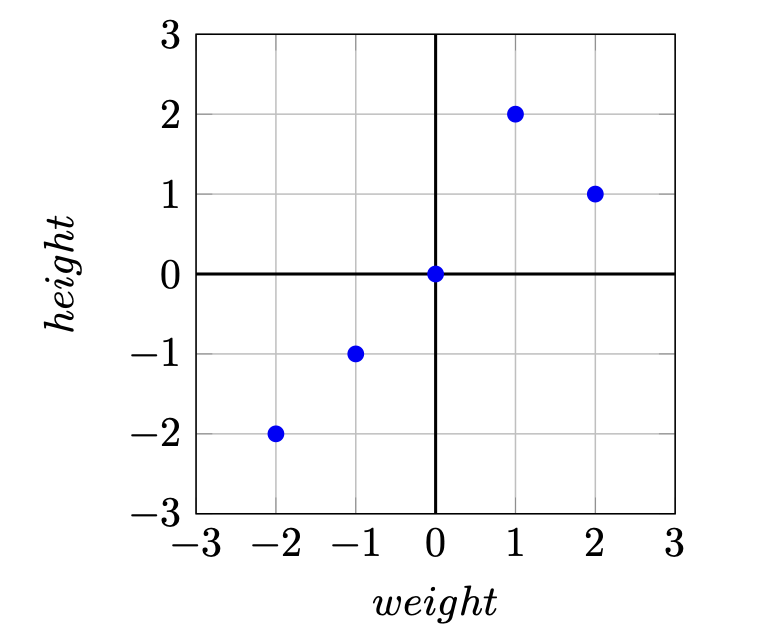
\includegraphics[width=0.5\textwidth]{601-2-1-1.png}
\end{center}

\textcolor{blue}{
The principal loading $u_1 = \frac{1}{\sqrt{2}}(1,1)^T$.\\
\\
The score of each point is the location of the point's projection onto the loading vector. The scores are $-2\sqrt{2}, -\sqrt{2}, 0, \frac{3}{2}\sqrt{2}, \frac{3}{2}\sqrt{2}$.
}

\subsection{Optimization and Solutions for PCA}
\begin{enumerate}
    \item \textbf{For $k = 1$ case}:\\
    We only have one projecting direction $u_1\in \R^q$ with $u_1^Tu_1 = 1$. We project centered data $y_i \rightarrow(u_1u_1^T)y_i = u_1(u_1^Ty_i) = u_iX_{i1}$.\\
    The goal of PCA is to maximize the variance of $X_{i1}, \dots, X_{ik}$, that is, to solve \[\underset{u_1\in\R^q}{\max}\frac{1}{n}\sum_{i=1}^n(X_i - \bar{X})^2 \quad s.t.\;u_1^Tu_1 = 1\] \[=\underset{u_1\in\R^q}{\max}\frac{1}{n}\sum_{i=1}^n(u_1^Ty_i - u_1^T\bar{y})^2 \quad s.t.\;u_1^Tu_1 = 1\]
    \textcolor{blue}{
    We know \[\frac{1}{n}\sum_{i=1}^n(u_1^Ty_i - u_1^T\bar{y})^2 = \frac{1}{n}\sum_{i=1}^nu_1^T(y_i-\bar{y})(y_i-\bar{y})^Tu_1\]
    \[ = u_1^T\left(\frac{1}{n}\sum_{i=1}^n(y_i-\bar{y})(y_i-\bar{y})^T\right)u_1 = u_1^TSu_1\]
    where $S$ is the sample covariance matrix $S = \frac{1}{n}\sum_{i=1}^n(y_i-\bar{y})(y_i-\bar{y})^T$.\\
    }
    Then the optimization problem becomes \[\underset{u_1\in\R^q}{\max} u_1^TSu_1 \quad s.t.\;u_1^Tu_1 = 1\]
    
    We introduce Lagrange multiplier:
    \[\underset{u_1\in\R^q}{\max}u_1^TSu_1 -\lambda(u_1^Tu_1-1)\]
    Take derivative w.r.t. $u_1$, we obtain 
    \[2Su_1 - 2\lambda u_1 = 0\]
    that is $Su_1  = \lambda u_1$, which indicates $\lambda$ is the eigenvalue of $S$ and $u_1$ is the corresponding eigenvector.\\
    Then replace $u_1^TSu_1 -\lambda(u_1^Tu_1-1)$ with $Su_1  = \lambda u_1$, the problem becomes
    \[\underset{u_1\in\R^q}{\max}u_1^T\lambda u_1 -\lambda(u_1^Tu_1-1) = \underset{u_1\in\R^q} \lambda\]
    This means $\lambda$ is the largest eigenvalue of matrix $S$ and $u_1$ is the corresponding eigenvector.
    
    \item \textbf{For general cases $k$}:\\
    The subspace is $U = [u_1, \dots, u_k]_{q\times k}$, $U^TU = I_k$, and here we project $y_i \rightarrow U_{q\times k}U^Ty_i = u_1X_{i1}+\dots+u_kX_{ik}$. \\
    The optimization problem becomes
    \[\underset{U\in\R^{q\times k}}{\max} \sum_{j=1}^k u_j^TSu_j \quad s.t.\;U^TU = I_k\]
    that is, $u_i^Tu_i = 1$ and $u_i^Tu_j = 0, \; \forall i \ne j$.\\

    \textbf{examples 2.1.2}\\
    Show that maximizing the variance of scores is equivalent to
minimizing projection error.\\

\textcolor{blue}{
\[\underset{U}{\min} \| Y - YUU^T \|_F^2\]\[ = \underset{U}{\min}  tr \big( (Y - YUU^T)^T (Y - YUU^T) \big)\]
\[= \underset{U}{\min} \, tr \big( Y^T Y - Y^T YUU^T - UU^T Y^T Y + UU^T Y^T YUU^T \big)\]
\[= \underset{U}{\min} tr \big( Y^T Y - Y^T YUU^T \big)\quad (\because tr(UU^T Y^T YUU^T) = tr(UU^T Y^T Y))\]
\[= \underset{U}{\max} tr \big( Y^T YUU^T \big) = \underset{U}{\max} tr \big(U^T Y^T YU \big) \]\[= \underset{U}{\max} tr\big( U^T S U \big) = \underset{U}{\max} \sum_{i=1}^k u_i^T S u_i\]
}

\textbf{Solutions to general cases}:\\
\begin{itemize}
    \item \textbf{Method 1: solve them iteratively}:\\
    
    Step 1: solve $\underset{u_1\in\R^q}{\max} u_1^TSu_1 \quad s.t.\;u_1^Tu_1 = 1$;\\
    Step $j\; (j\ge 2)$: solve $\underset{u_j\in\R^q}{\max} u_j^TSu_j \quad s.t.\;u_j^Tu_j = 1, \;u_k^Tu_j = 0, \; \forall k<j$.

    \item \textbf{Method 2: solve them simultaneously (Eigen-Decomposition)}:\\

    \[\underset{U\in\R^{q\times k}}{\max} \sum_{j=1}^k u_j^TSu_j - \sum_{j=1}^k\lambda (u_j^Tu_j - 1) - \sum_{j\ne k}u_j^Tu_k\]
    It is equivalent to 
    \[\underset{U\in\R^{q\times k}}{\max} tr(U^TSU) - tr(\Lambda(U^TU-I_k)), \quad \Lambda \text{ symmetric}\]
    Take derivative:
    \[2SU-2U\Lambda = 0 \Rightarrow SU = U\Lambda \Rightarrow \Lambda = U^TSU\]
    Eigen-Decomposition: let $\Lambda = ODO^T$, $O^TO = I$, where $D$ is diagonal. Then $SUO = UOD$.\\
    If we let $U^* = UO$, we then have $SU^* = U^*D$, which means
    \[S = U^*DU^{*T},\quad U^{*T}U^* = I\]
    $U^*$ is the set of eigenvectors of $S$ with eigenvalues $d_1,\dots,d_k$.\\
    The problem becomes 
    \[\underset{U^*\in\R^{q\times k}}{\max} \sum_{j=1}^k u_j^{*T}Du_j^* \quad s.t.\;U^{*T}U^* = I_k\]

    In computing, we first perform eigen-decomposition on $S$ and get $O$ and $D$. Then we solve the optimization problem and get $U^*$. The loading matrix is given by $U = U^*O^T$.

    \item \textbf{Method 3: Singular Value Decomposition (SVD)}:\\\label{sec:S}
    In method 2 we perform eigen-decomposition on sample covariance matrix $S$. In method 3, we directly use SVD on the centered data matrix $\bar{Y}$.\\

    Let $\bar{Y}$ denotes the centered data: \[
    \bar{Y}_{n\times q} = \begin{pmatrix}y_1-\bar{y}
 \\\vdots
 \\y_n-\bar{y}

\end{pmatrix}
    \]
Let $\bar{Y}_{n\times q} = U_{n\times q}D_{q\times q}V_{q\times q}^T$, where 
\[U_{n\times q}: \text{ orthogonal, } U^TU = I_q. \text{ Columns of $U$ are left singular vectors;}\]
\[V_{q\times q}: \text{ orthogonal, } V^TV = I_q. \text{ Columns of $V$ are right singular vectors;}\]
\[D_{q\times q}: \text{ diagonal, } D = \begin{pmatrix}  
  d_1 & 0 & \cdots & 0 \\  
  0 & d_2 & \cdots & 0 \\  
  \vdots & \vdots & \ddots & \vdots \\  
  0 & 0 & \cdots & d_q  
\end{pmatrix}. d_1\ge \dots \ge d_q. \]
\textbf{Note}: The $D$ here is not the same as the one in Method 2 !

Sample covariance \[S = \frac{1}{n}\bar{Y}^T\bar{Y} = \frac{1}{n}VDU^TUDV^T = \frac{1}{n}VD^2V^T\]

Therefore, the eigenvalues of $S$ are $\frac{d_i^2}{n}$; the eigenvectors are contained in $V$. The first $k$ columns of $V$ are the principal loadings.
\end{itemize}

\subsection{Properties of PCA}
Consider population version: 
\[\underset{U\in\R^{q\times k}}{\max} tr(U^T\Sigma U) \quad s.t.\;U^TU = I_k\]
where $U$ contains the top k eigenvectors of $\Sigma$.
\begin{itemize}
    \item For the PCA scores $X = YU$, \[E(X) = E(Y)U = 0\]\[cov(X) = U^Tcov(Y)U = U^T\Sigma U = \begin{pmatrix}  
  \lambda_1 & 0 & \cdots & 0 \\  
  0 & \lambda_2 & \cdots & 0 \\  
  \vdots & \vdots & \ddots & \vdots \\  
  0 & 0 & \cdots & \lambda_k  
\end{pmatrix} \] where $\lambda_1 \ge \dots \ge \lambda_k$ are the top k eigenvalues.
    \item When $k = q$, the total variance is $tr(\Sigma) = \sum_{j=1}^k \lambda_j$. The $j$-th component accounts for $\frac{\lambda_j}{\sum_{j=1}^k \lambda_j}$ proportion of variance.
    \item Another way to look at PCA:\\
    Approximate data by $\tilde{y_i} = \mu+UX_i$ and our goal is to find the best linear combination that gives minimum aprroximation error.
\end{itemize}
    
\end{enumerate}

\subsection{Probabilistic PCA (for a spiked covariance model)}
This can be thought of a MLE of latent variable model:
\[Y_{q\times 1} = \mu_{q\times 1} + \Lambda_{q\times k} X_{k\times 1}+ W_{q\times 1}\]
where $W \perp X, \quad W \sim N_q(0,\sigma^2I_q), \quad X\sim N_k(0, I_k)$ are latent variables. \\
Therefore, we have $Y\sim N_q(\mu, \sigma^2 I_q+\Lambda \Lambda^T)$ where $\Lambda\Lambda^T$ has low rank ($k \ll q$). The column space of $\Lambda$ corresponds to the top k eigenvectors of $\Sigma = \sigma^2 I_q+\Lambda \Lambda^T$.
\begin{enumerate}
    \item When $k=1$, $y \sim N_q(\mu, \sigma^2 I_q+\Lambda \Lambda^T)$, where$\Lambda$ is a $q$-dim vector.\\
    The first PCA vector is $\frac{\Lambda}{\|\Lambda\|_2}$ and the variance is $\sigma^2+ \|\Lambda\|_2^2$.
    \textcolor{blue}{
    \begin{proof}[Proof sketch]
        \[(\sigma^2 I_q+\Lambda \Lambda^T)\frac{\Lambda}{\|\Lambda\|_2} = (\sigma^2+ \|\Lambda\|_2^2)\frac{\Lambda}{\|\Lambda\|_2}\]
    \end{proof}}
    \item $k$-dimension:\\
    The log likelihood is given by
    \[\ell = \log L = -\frac{nq}{2}\log(2\pi) - \frac{n}{2} \log|\Sigma| - \frac{1}{2}\sum_{i=1}^n (y_i-\mu)^T \Sigma^{-1}(y_i - \mu)\]
    We let $\frac{\partial \ell}{\partial \mu} = 0$ and get the MLE of $\mu$ is $\hat{\mu} = \bar{y}$.
    After we subtract $\bar{y}$ and set $S = \sum_{i=1}^n (y_i-\bar{y})(y_i - \bar{y})^T$, the log likelihood becomes
    \[\ell = -\frac{n}{2}[q\log(2\pi) + \log|\Sigma| + tr(\Sigma^{-1}S)]\]
    We can solve this using EM algorithm, which will be introduced in Chapter 4.
\end{enumerate}

\begin{referencebox}
    \begin{itemize}
        \item Chapter 17.2, \textit{PRML};
        \item Tipping, M. E., \& Bishop, C. M. (1999). Probabilistic principal component analysis. \textit{Journal of the Royal Statistical Society Series B: Statistical Methodology}, 61(3), 611-622.
    \end{itemize}
\end{referencebox}



\subsection{PCA for High-dimensional data ($n<q$)}
Same as 2.1.2 Method 3(~\ref{sec:S}), we use $S_{q\times q} = \frac{1}{n}\bar{Y}^T\bar{Y}$ notation. $S$ has $q$ eigenvalues but at least $q-n$ are 0 because of rank. The computational cost for finding $q$ eigenvectors is $O(q^3)$.\\
So we consider $G_{n\times n} = \frac{1}{n}\bar{Y}\bar{Y}^T$.\\
Suppose the eigenvectors of $S$ are $u_1, \dots, u_k$, we have $Su_j = \lambda_j u_j,\quad j = 1,\dots, k$.\\
Multiply both sides by $\bar{Y}$:
\[\frac{1}{n}\bar{Y}\bar{Y}^T\bar{Y}u_j = \lambda_j\bar{Y}u_j\]
which means 
\[G\bar{Y}u_j = \lambda_j\bar{Y}u_j\]
Let $\gamma_j = \bar{Y}u_j$, then 
\[G\gamma_j = \lambda_j\gamma_j\]
$\gamma_j$ are the eigenvectors for $G$. $\|\gamma_j\| = 1$. Thus the computational cost to get $\gamma_j$'s is $O(n^3)<O(q^3)$.

\[u_j = \frac{\bar{Y}^T\gamma_j}{\|\bar{Y}^T\gamma_j\|_2} = \frac{1}{\sqrt{n\lambda_j}}\bar{Y}^T\gamma_j\]
\textcolor{blue}{
\begin{proof}[Proof sketch]
    \[\|\bar{Y}^T\gamma_j\|_2^2 = \gamma_j^T\bar{Y}\bar{Y}^T\gamma_j = n\lambda_j\]
\end{proof}
}

\newpage
\section{Sparse PCA}
For data $Y_{q\times 1} = (y-1, \dots, y_q)$. Assume $u_1, \dots, u_k$ to be sparse, e.g., $u_1 = (\frac{\sqrt{2}}{2},\frac{\sqrt{2}}{2},0,\dots, 0)$.
\subsection{Method 1: Based on LASSO}
Start with $u_1$:
\[u_1 = \arg\underset{u_1}{\max}\; u_1^TSu_1, \quad s.t. \;u_1^Tu_1 = 1 \; and \; \|u_1\|\le t\]
Then solve $u_2,\dots, u_k$ sequentially.
\begin{referencebox}
    Jolliffe, I.T., Trendafilov, N.T., \& Uddin, M. (2003). A Modified Principal Component Technique Based on the LASSO. \textit{Journal of Computational and Graphical Statistics}, 12(3), 531–547.
\end{referencebox}

\subsection{Method 2: Hui Zou's method}
The PCA method becomes
\[\underset{\Theta, \mu}{\min}\sum_{i=1}^n\|y_i - \Theta U^Ty_i\|_2^2+\lambda_1\|U\|_1+\lambda_2\|U\|_2^2 \quad s.t. \;U^TU = I_k\]
First, we fix $\Theta$ and solve $U$; then we fix $U$ and solve $\Theta$. Repeat the procedure until they reach convergence.
\begin{referencebox}
    Zou, H., Hastie, T., \& Tibshirani, R. (2006). Sparse principal component analysis. \textit{Journal of computational and graphical statistics}, 15(2), 265-286.
\end{referencebox}

\subsection{Method 3: Fantope Projection for PCA}
The problem becomes
\[\max\; tr(SX) - \lambda\|X\|_{1,1}\quad s.t. \; X\in \mathcal{F}^k\]
where $\|X\|_{1,1} = \sum_{j,k}|X_{jk}| $ and $\mathcal{F}^k  = \{X: 0\le X\le I, tr(X) = k\}$.\\

This method is \textbf{CONVEX} and all other sparse PCA methods are not!
Thus we can find the optimal value.

\paragraph{Assumptions}
\begin{itemize}
    \item $S, \Sigma$ are symmetric;
    \item Let $\delta(\Sigma) = \lambda_k(\Sigma) - \lambda_{k+1}(\Sigma)>0$;
    \item Sparsity - projection $\Pi$: the projection of data $X$ onto subspace spanned by eigenvectors of $\Sigma$ corresponding to $k$ largest eigenvalues of $\Sigma$.\\
    This satisfies \[\|\Pi\|_{2,0}\le c \;\text{ or } \;\|diag(\Pi)\|_0\le c\] where $c$ is a constant, $\|\Pi\|_{2,0} = \sum_{i=1}^n \mathbb{I}_{\{\|\Pi_{i,:}\|_2 \neq 0\}}$ is the number of non-zero rows in $\Pi$, $ \|diag(\Pi)\|_0 = \sum_{i=1}^n \mathbb{I}_{\{\Pi_{ii} \neq 0\}}$ is the number of non-zeros diagonal entries in $\Pi$.
\end{itemize}

\paragraph{Theorem} If $\lambda > \|\Pi\|_{\infty, \infty}$ and $S \ge \|\Pi\|_{2,0}$, then 
\[\|\hat{X} - \Pi\|_F \le \frac{4S\lambda}{\delta}\]
where $\delta = \lambda_k(\epsilon) - \lambda_{k+1}(\epsilon)>0$, $\left \| \mathrm {A}    \right \| _{\infty, \infty}=\underset{1\le i\le m}{\max} \sum_{j=1}^{n}\left | a_{ij} \right |$.\\

\textcolor{blue}{
\begin{proof}
    Let $\hat{X}$ be the optimal solution of 
    \[\min\; -tr(SX) + \lambda\|X\|_{1,1}\quad s.t. \; X\in \mathcal{F}^k\]
    \[
-tr(S\hat{X}) + \lambda \| \hat{X}\|_{1,1} \leq - tr(S\Pi) + \lambda \| \Pi \|_{1,1}
\]
\[
\Rightarrow 0 \leq tr(S(\hat{X} - \Pi)) + \lambda \| \Pi \|_{1,1} - \lambda \|\hat{X} \|_{1,1}
\]
Let \(\hat{\Delta} = \hat{X} - \Pi\), then:
\[
0 \leq tr(S\hat{\Delta}) + \lambda \| \Pi \|_{1,1} - \lambda \| \hat{\Delta} + \Pi \|_{1,1}
\]
\[
0 \leq tr(S\hat{\Delta}) - \lambda ( \| \hat{\Delta} + \Pi \|_{1,1} - \| \Pi \|_{1,1} )
\]
\textbf{By Lemma in Vu et al. (2013)}, we have $\frac{\delta}{2} \| \hat{\Delta} \|_F^2 \le -tr(\Sigma\hat{\Delta})$. Then:
\[
\frac{\delta}{2} \| \hat{\Delta} \|_F^2 + tr(\Sigma\hat{\Delta}) \leq tr(S\hat{\Delta}) - \lambda ( \| \hat{\Delta} + \Pi \|_{1,1} - \| \Pi \|_{1,1} )
\]
\[
\frac{\delta}{2} \| \hat{\Delta} \|_F^2 \leq tr(S - \Sigma) \hat{\Delta} - \lambda ( \| \hat{\Delta} + \Pi \|_{1,1} - \| \Pi \|_{1,1} )
\]
Using Hölder’s inequality:
\[
\frac{\delta}{2} \| \hat{\Delta} \|_F^2 \leq \| S - \Sigma \|_{\infty, \infty} \| \hat{\Delta} \|_{1,1} - \lambda ( \| \hat{\Delta} + \Pi \|_{1,1} - \| \Pi \|_{1,1} )
\]
\[
\leq \lambda( \| \hat{\Delta} \|_{1,1} - \| \hat{\Delta} + \Pi \|_{1,1} + \| \Pi \|_{1,1} )
\]
Consider
\[
\| \hat{\Delta} \|_{1,1} - \| \hat{\Delta} + \Pi \|_{1,1} + \| \Pi \|_{1,1} \]\[= \| \hat{\Delta}_J \|_{1,1} - \| \hat{\Delta}_J + \Pi_J \|_{1,1} + \| \Pi_J \|_{1,1}
\]
where \( J \) is the subset of indices of nonzero entries of \( \Pi \), hence
\[\le 2\| \hat{\Delta}_J \|_{1,1}\]
Therefore, 
\[\frac{\delta}{2} \| \hat{\Delta} \|_F^2 \le 2\lambda\| \hat{\Delta}_J \|_{1,1}\]
Because $J$ has at most $S^2$ entries,
\[\frac{\delta}{2} \| \hat{\Delta} \|_F^2 \le 2\lambda\| \hat{\Delta}_J \|_{1,1} \le 2S\lambda\| \hat{\Delta}_J \|_{F}\le 2S\lambda\| \hat{\Delta} \|_{F}\]
So \[\frac{\delta}{2} \| \hat{\Delta} \|_F \le 2S\lambda\]
which indicates \[\|\hat{X} - \Pi\|_F \le \frac{4S\lambda}{\delta}\]
\end{proof}
}

\begin{referencebox}
    Vu, V. Q., Cho, J., Lei, J., \& Rohe, K. (2013). Fantope projection and selection: A near-optimal convex relaxation of sparse PCA. \textit{Advances in neural information processing systems}, 26.
\end{referencebox}


\subsection{Method 4: Truncated power method}
In this method, the problem becomes 
\[\arg\underset{u\in\R^q}{\max} \;u^TSu, \quad s.t. \;u^Tu = 1, \;\|u\|_0 \le S\]
Here we have $\|\hat{u}-u\|_2 \le c\sqrt{S\log(\frac{q}{n})}$, which is better the theorem's result above ($\|\hat{u}-u\|_2 \le \frac{4S}{\delta}\sqrt{\log(\frac{q}{n})}$) when we choose $\lambda = \sqrt{\log(\frac{q}{n})}$ because here $S$ lies inside the square root. 

\begin{referencebox}
    Yuan, X. T., \& Zhang, T. (2013). Truncated power method for sparse eigenvalue problems. \textit{The Journal of Machine Learning Research}, 14(1), 899-925.
\end{referencebox}

\newpage
\chapter{Factor Analysis}
\section{Factor Model}
\subsection{Model}
It is a model-based approach for dimension reduction. \\
Assume data lie in a low-dimension linear space. The model is \[Y_{q\times 1} = \mu_{q\times 1} + \Lambda_{q\times k} X_{k\times 1}+ W_{q \times 1}\]
where $W\perp X$, $X\sim N_k(0, I_k)$, $W\sim N_q(0,\Psi)$ and $\Psi = \begin{pmatrix}  
  \psi_1 & 0 & \cdots & 0 \\  
  0 & \psi_2 & \cdots & 0 \\  
  \vdots & \vdots & \ddots & \vdots \\  
  0 & 0 & \cdots & \psi_q  
\end{pmatrix} $ where $\psi_i>0,\;\;\;i = 1,\dots,q$.\\
In this model, $\Lambda$ is the loading matrix, $X$ is the factors and $W$ is the random noise.\\

Under the Gaussian assumption, 
\[\begin{pmatrix}
 X\\
Y
\end{pmatrix}\sim N(\begin{pmatrix}
 0\\
0
\end{pmatrix}, \begin{pmatrix}
 I & \Lambda\\
 \Lambda^T &\Lambda\Lambda^T+\Psi\end{pmatrix})\]
where $X$ is latent and $Y$ can be observed. It is equivalent to $Y\sim N(0,\Lambda\Lambda^T+\Psi)$.

\textbf{The GOAL} of Factor model is to estimate $\mu, \Lambda, \Psi$ using only $Y_1, \dots, Y_n$.

\subsection{Estimation}
The log likelihood function is given by
\[\ell(\theta|y) = -\frac{n}{2}\log\det(\Lambda\Lambda^T+\Psi)-\frac{1}{2}\sum_{i=1}^n(y_i - \mu)^T(\Lambda\Lambda^T+\Psi)^{-1}(y_i - \mu)+c\]

\begin{enumerate}
    \item $\mu$:\\
    \[\frac{d \ell}{d \mu} = -\sum_{i=1}^n (\Lambda\Lambda^T+\Psi)^{-1}(y_i - \mu) = 0\]
    So the MLE of $\mu$ is easy to calculate, which is $\hat{\mu} = \bar{y}$.\\
    \\
    However, the MLE's for $\Lambda$ and $\Psi$ are challenging. (they are not identifiable!)
    \item $\Lambda$:\\
    No unique $\Lambda$ since $\ell(\theta|y)$ depends on $\Lambda$ only through $\Lambda\Lambda^T$. If we have an orthogonal matrix $R$ where $RR^T = I$, then $(\Lambda R)(\Lambda R)^T = \Lambda\Lambda^T$.\\

    To make $\Lambda$ identifiable:\\
    if $\Lambda$ is constrained to satisfy $\Lambda_{q\times k} = \begin{pmatrix}
 1 &  \cdots&0\\
 & \ddots & \vdots\\
 \star &  & 1\\
  &  & \\
  & \star &\\
  &  &
\end{pmatrix}$ (add $\frac{k(k+1)}{2}$ constraints), then $\Psi$ is diagonal, $\Lambda, \mu, \Psi$ are all identifiable.
\end{enumerate}


\begin{referencebox}
    \begin{itemize}
        \item Chapter 14, \textit{An Introduction to Multivariate Statistical Analysis} by T.W.Anderson;
        \item Bai, J., \& Li, K. (2012). Statistical analysis of factor models of high dimension.
    \end{itemize}
\end{referencebox}

\subsection{Select number of factors $k$}
\paragraph{Upper bound of $k$}
The degree of freedom is given by
\[df = \frac{q(q+1)}{2} - [q(k+1) - \frac{k(k-1)}{2}] = \frac{1}{2}[(q-k)^2 - (q+k)]\]
in which the first one is from symmetric covariance matrix of $Y$ $\Sigma_{q\times q}$ and the second one is from $\Psi + \Lambda\Lambda^T$ while $q$ is from $\Psi$, $qk$ is from $\Lambda$, $\frac{k(k-1)}{2}$ means the number of elements that constrained to be 0 in $\Lambda$.\\
Because we need $df > 0$, we get the upper bound of $k$. 

\paragraph{methods to select $k$}
\begin{itemize}
    \item scree plot;
    \item parallel analysis;
    \item mode-based approach: AIC, BIC, \dots;
    \item Likelihood Ratio Test (LRT).
\end{itemize}
We will then discuss LRT specifically.

\paragraph{LRT framework}
\begin{itemize}
    \item Step 1: $H_0: k = 0$ V.S. $H_1: k>0\; $, i.e., $\;H_0: \Sigma = \Psi$ V.S. $H_1: \Sigma \ne \Psi$.\\

    If we reject $H_0$, 
    \item Step 2: $H_0: k = 1$ V.S. $H_1: k>1\;$, \\i.e., $\;H_0: \Sigma = \Psi+\Lambda\Lambda^T $ V.S. $ H_1: \Sigma \ne \Psi+\Lambda\Lambda^T$.\\

    If we reject $H_0$, 
    \item Step 3: $H_0: k = 2$ V.S. $H_1: k>2$.\\

    Stop when we fail to reject $H_0$.

    Test statistics: 
    \[LRT = \frac{\underset{\Theta_0}{\sup}L(\mu, \Sigma)}{\underset{\Theta_1}{\sup}L(\mu, \Sigma)}\]
    and \[-2\log LRT \overset{d}{\rightarrow} \chi^2_{df}\]
\end{itemize}

\subsection{Estimate latent factors $X$}
Suppose $\hat{\mu}, \hat{\lambda}, \hat{\Psi}$, we want to estimate the latent factors $X$.

\paragraph{Lemma} If 
\[\begin{pmatrix}
 X_1\\
X_2
\end{pmatrix}\sim N(\begin{pmatrix}
 \mu_1\\
\mu_2
\end{pmatrix}, \begin{pmatrix}
 \Sigma_{11} & \Sigma_{12}\\
 \Sigma_{21} & \Sigma_{22} \end{pmatrix})\]
 Then the conditional distribution is 
 \[X_1|X_2 \sim N(\mu_1+ \Sigma_{12}\Sigma_{22}^{-1}(X_2 - \mu_2), \Sigma_{11} - \Sigma_{12}\Sigma_{22}^{-1}\Sigma_{21})\]
\\
\\
 In this case, $X|Y \sim N(E(X|Y), var(X|Y))$, where 
 \[E(X|Y) = 0 + \Lambda^T(\Psi + \Lambda\Lambda^T)^{-1}(Y - \mu) = (I+\Lambda^T\Psi^{-1}\Lambda)^{-1}\Lambda^T\Psi^{-1}(Y-\mu)\]
 which is like Ridge regression.

\begin{notionbox}[Note]
    Sherman-Morrison identity: 
    \[(A+ uv^T)^{-1} = A^{-1} - \frac{A^{-1}uv^TA^{-1}}{1+v^TA^{-1}u}\]
    Woodbury identity: 
    \[(A+UCV^T)^{-1} = A^{-1} - A^{-1}U(C^{-1}+VA^{-1}U)^{-1}VA^{-1}\]
\end{notionbox}


\newpage
\section{Comparison between Probabilistic PCA and Factor Analysis}
\subsection{Model}

\paragraph{Probabilistic PCA}
The model is  \[Y = \Lambda X+W\]
where $W\sim N(0,\sigma^2 I)$, which indicates the same variance;

\paragraph{Factor Analysis}
The model is \[Y = \Lambda X+W\]
where $W\sim N(0,\Psi)$, and $\Psi$ is diagonal, which means we have different variance for each dimension.

\subsection{Solution}

\paragraph{Probabilistic PCA}
The MLE's of PCA can be obtained by eigen-decomposition on the sample covariance matrix or SVD on the centered data.

\paragraph{Factor Analysis}
The MLE's of Factor model are often calculated by EM algorithm.

\subsection{Application}

\paragraph{Probabilistic PCA}
Used more in dimension reduction, data visualization and reconstruction. The goal is to find the direction with the maximum variance.

\paragraph{Factor Analysis}
Used more for discovering latent factors for the observed data.\\



\textbf{Note}: For both PCA and FA, $\Lambda$ can only be identified up to an orthonormal transformation, i.e., the solutions remains invariant to the rotation of $\Lambda$. Their solutions are not unique.












\newpage{}
\chapter{EM Algorithm}
\section{Motivation and Intuition for EM Algorithm}
\subsection{Motivation}
Now we have latent variables $X_1, \dots, X_n$ and observed data $Y_1,\dots, Y_n$. Suppose $(Y_i, X_i)$ is sampled from $ p(y,x|\theta)$ where $\theta$ is unknown. \\
The \textbf{GOAL} is to find the MLE of $\theta$ given only the observed data $Y_1,\dots, Y_n$, which is to maximize the marginal log likelihood
\[\ell (\theta|y) = \sum_{i=1}^n \log p(y_i|x_i,\theta) = \sum_{i=1}^n \log \int_{\mathcal{X}_i}p(y_i,x_i|\theta)dx_i\]
\[=\sum_{i=1}^n \log \int_{x_i}p(x_i)p(y_i|x_i,\theta)dx_i\]
and we use iterative approach to solve this problem.


\paragraph{Example 4.1.1: Finite mixture model}

\begin{itemize}
    \item Let \( f(y|\psi) \) be a distribution parameterized by \( \psi \).\( Y \) is sampled from one of \( f(y|\psi_k) \), \( k = 1, \dots, K \).
    \item \( X \in \{1, \dots, K\} \) indicates which distribution \( Y \) is sampled from. \( X = k \) with probability \( \pi_k \).
\end{itemize}

\[
X \sim \text{Multinomial}(\pi_1, \dots, \pi_K), \quad Y | X = k \sim f(y|\psi_k).
\]

\begin{itemize}
    \item Unknown parameters we want to estimate: \( \theta = (\pi, \psi) \).
    \item Consider \( (y_1, x_1), \dots, (y_n, x_n) \) i.i.d. sampled from \( p(y, x | \theta) \). We only observe \( y_1, \dots, y_n \).
\end{itemize}

Express the marginal log likelihood in terms of $(\pi, \psi)$.

\textcolor{blue}{
\[\ell (\theta|y) = \sum_{i=1}^n \log p(y_i|\theta)\]
\[= \sum_{i=1}^n \log \sum_{k=1}^K p(y_i, x_i = k|\theta)\]
\[= \sum_{i=1}^n \log \sum_{k=1}^K p(x_i = k|\theta)p(y_i|x_i = k,\theta)\]
\[ = \sum_{i=1}^n \log (\sum_{k=1}^K\pi_k f(y_i|\psi_k))\]
}

\subsection{Intuition}
\paragraph{E-Step}
Since maximizing nonconvex $\ell (\theta|y)$ is hard computationally, we optimize an easy-to-work-with surrogate function $\mathcal{F}(\theta, q)$ instead of $\ell (\theta|y)$. \\
Here the surrogate function $\mathcal{F}(\theta, q)$ is the lower bound for $\ell (\theta|y)$:\\
\[\forall \theta, \mathcal{F}(\theta, q) \le \ell (\theta|y), \forall q\]
\[\underset{\theta}{\max}\ell (\theta|y) = \underset{\theta}{\max}\underset{q}{\max} \mathcal{F}(\theta, q)\]
In $t$-th iteration, the function is based on $\theta^{(t-1)}$. The E-step can be viewed as solving
\[q^{(t)} = \arg\underset{q\in Q}{\max}\mathcal{F}(\theta^{(t-1)}, q)\]
which is solving the optimal $q$ with $\theta$ fixed. 
\paragraph{M-Step}
we maximize the surrogate function $\mathcal{F}(\theta, q)$ to update $\theta^{(t-1)}$ to $\theta^{(t)}$. This step can be written as \[\theta^{(t)} = \arg\underset{\theta}{\max}\mathcal{F}(\theta, q^{(t)})\]
which is solving the optimal $\theta$ with $q$ fixed.\\

Then the constraints on the surrogate function above become
\[\mathcal{F}(\theta^{(t-1)},q)\le \ell(y|\theta^{(t-1)})\]
\[\mathcal{F}(\theta^{(t-1)},q^{(t)}) = \ell(y|\theta^{(t-1)})\]

\paragraph{Note}
EM Algorithm guarantees that $\ell(\theta^{(t)}|y)$ never decreases. Each iteration pushes up the lower bound. 
\textcolor{blue}{
\begin{proof}[Proof Sketch]
    \[
\ell(\theta^{(t-1)}|y) = \mathcal{F}(\theta^{(t-1)}, q^{(t)}) \]\[\leq \mathcal{F}(\theta^{(t)}, q^{(t)})\]\[ = \mathcal{F}(\theta^{(t)}, q^{(t+1)}) \]\[= \ell(\theta^{(t)}|y)\]
\end{proof}
}


\newpage
\section{Interpretation for EM Algorithm}
Next we prove that the marginal likelihood has a lower bound.
\[\ell(\theta|y) = \log p(y_1, \dots, y_n|\theta)\]
\[=\log p(y|\theta) \int_\mathcal{X}q(x)dx\quad q(x)\;is\;a\;pdf\]
\[=\int_\mathcal{X}\log p(y|\theta)q(x)dx\]
\[=\int_\mathcal{X}\log[\frac{q(x)}{q(x)}\cdot \frac{p(y,x|\theta)}{p(x|y,\theta)}]q(x)dx\]
\[=\int_\mathcal{X}\log[\frac{p(y,x|\theta)}{q(x)}]q(x)dx+\int_\mathcal{X}\log[\frac{q(x)}{p(x|y,\theta)}]q(x)dx\]
\[ = \mathcal{F}(\theta,q)+D_{KL}(q\|p(\cdot|y,\theta))\]


\begin{notionbox}[KL Divergence]
    KL Divergence is represented by $D_{KL}(q\|p) = \int_\mathcal{X}\log(\frac{q(x)}{p(x)})q(x)dx$. \\
    Next we will prove KL Divergence is positive:
    \[D_{KL}(q\|p) = \int_\mathcal{X}\log(\frac{q(x)}{p(x)})q(x)dx\]
    \[= E_{X\sim q(\cdot)}\log(\frac{q(x)}{p(x)})= -E_{X\sim q(\cdot)}\log(\frac{p(x)}{q(x)})\]
    \[= -\int_\mathcal{X}\log(\frac{p(x)}{q(x)})q(x)dx\]
    \[\ge -\log \int_\mathcal{X}\frac{p(x)}{q(x)}\cdot q(x)dx \quad (Jensen's \; Inequality)\]
    \[ = -\log \int_\mathcal{X}p(x)dx = - \log(1) = 0\]
    and "=" holds $\iff$ $p(x) = q(x)$.
\end{notionbox}

Because KL Divergence is positive, the lower bound of log likelihood is $\mathcal{F}(\theta,q) = \int_\mathcal{X}\log[\frac{p(y,x|\theta)}{q(x)}]q(x)dx = E_{X\sim q(\cdot)}\log(\frac{p(x,y|\theta)}{q(x)})$, called \textbf{Evidence Lower Bound (ELBO)}.\\

Usually, taking max over $\mathcal{F}(\theta,q)$ is easier than $\ell(\theta|y)$, and we often calculate $E_{X\sim q(\cdot)}\log p(x,y|\theta)$ instead because $E_{X\sim q(\cdot)}\log q(x)$ is independent of $\theta$.

\begin{referencebox}
    \begin{itemize}
        \item Dempster, A. P., Laird, N. M., \& Rubin, D. B. (1977). Maximum likelihood from incomplete data via the EM algorithm. \textit{Journal of the royal statistical society: series B (methodological)}, 39(1), 1-22;
        \item Chapter 9, \textit{PRML}.
    \end{itemize}
\end{referencebox}

\newpage
\section{EM Algorithm}
\paragraph{E-Step}
In this step we need to maximize $\mathcal{F}(\theta^{(t-1)},q)$:\\
\begin{itemize}
    \item First we calculate the maximized surrogate function $q$: $q(x)^{(t)} = p(x| y, \theta^{(t-1)})$;
    \textcolor{blue}{
    \begin{proof}[Proof sketch]
        maximize $\ell (\theta|y) \iff D_{KL} = 0 \iff q(x)^{(t)} = p(x| y, \theta^{(t-1)})$.
    \end{proof}
    }
    \item Then we calculate $ E_{X\sim q^{(t)}(\cdot)}\log p(x,y|\theta) = \int\log p(x,y|\theta)q^{(t)}(x)dx$.
\end{itemize}

\paragraph{M-Step}
In this step we need to maximize $\mathcal{F}(\theta,q^{(t)})$:\\
We need to calculate $\theta^{(t)} = \arg \underset{\theta}{\max}E_{X\sim q^{(t)}(\cdot)}\log p(x,y|\theta)$.


\begin{notionbox}[Note]
    EM Algorithm is a \textbf{Coordinate Ascent} algorithm. For maximizing the log likelihood:\\
    
    \textbf{E-Step}:
    update $q^{(t+1)} = \arg\underset{q}{\max}\mathcal{F}(\theta^{(t)}, q)$;\\
    
    \textbf{M-Step}: 
    update $\theta^{(t+1)} = \arg\underset{\theta}{\max}\mathcal{F}(\theta, q^{(t+1)})$
\end{notionbox}

\paragraph{Example 4.3.1: Bernoulli Mixture Model}
Consider a mixture model with \(K\) components. Each component \(k\) is parameterized by a Bernoulli distribution with success probabilities 
    \[\psi_k = (\psi_{k1}, \dots, \psi_{kd})\]
That is, a random vector \(\mathbf{Y} \in \{0,1\}^d\) from component \(k\) has independent entries, and each entry \(Y_j\) follows a Bernoulli distribution with success probability \(\psi_{kj}\).\\Mixing weight 
\[\pi = (\pi_1, \dots, \pi_K) \quad \text{where} \quad \sum_k \pi_k = 1\]
Each data point \(y_i \in \{0,1\}^d, \, i = 1, \dots, n\) is generated by:
\begin{enumerate}
        \item Selecting a component \(x_i \sim \text{Multinomial}(\pi)\).
        \item Sampling \(y_i \sim \text{Bernoulli}(\psi_{x_i})\).
    \end{enumerate}
Applications: black-white images with \(d = 64 \times 64\) pixels of \(K = 10\) digits.\\
\\

\textbf{Estimate} \(\theta = (\pi, \psi)\) \textbf{using EM algorithm.}\\

\textcolor{blue}{
The full likelihood of $(y_i, x_i),\quad i=1,\dots, n$ is 
\[p(y_i, x_i|\theta) = p(y_i|x_i,\theta)p(x_i|\theta)\]
\[ = \prod_{j=1}^d\psi_{x_i,j}^{y_{ij}}(1-\psi_{x_i,j})^{1-y_{ij}}\cdot \pi_{x_i}\]
\textbf{E-Step}: 
Recall $q_i = p(\cdot|y_i,\theta)$, 
\[q_i(k) = p(x_i = k|y_i,\theta)\]
\[=\frac{p(x_i = k,y_i|\theta)}{p(y_i|\theta)} = \frac{p(x_i = k,y_i|\theta)}{\sum_{k'=1}^Kp(x_i = k',y_i|\theta)} \]
\[ = \frac{\prod_{j=1}^d\psi_{kj}^{y_{ij}}(1-\psi_{kj})^{1-y_{ij}}\cdot \pi_k}{\sum_{k'=1}^K\prod_{j=1}^d\psi_{k'j}^{y_{ij}}(1-\psi_{k'j})^{1-y_{ij}}\cdot \pi_{k'}}\]
Recall for optimizing $\mathcal{F}(\theta,q)$, we only need to optimize $E_{X\sim q(\cdot)}\log p(x,y|\theta)$, which is 
\[\sum_{i=1}^nE_{X\sim q_i}\log p(x,y_i|\theta)\]
\[ = \sum_{i=1}^nE_{X\sim q_i}\{\log\pi_X+\sum_{j=1}^d[y_{ij}\log\psi_{x,j}+(1-y_{ij})\log(1-\psi_{x,j})]\}\]
\[ = \sum_{i=1}^n\sum_{k=1}^K q_i(k)\{\log\pi_k+\sum_{j=1}^d[y_{ij}\log\psi_{kj}+(1-y_{ij})\log(1-\psi_{kj})]\}\quad (\star)\]
\textbf{M-Step}:
\begin{itemize}
    \item $\pi$:
    Note that $\sum_k \pi_k = 1$, so we use Lagrangian method:
    \[L = (\star) + \lambda (1-\sum_{k=1}^K \pi_k)\]
    Take derivative:
    \[\frac{\partial L}{\partial \pi_k}  = \frac{1}{\pi_k}\sum_{i=1}^n q_i(k) - \lambda = 0 \quad (\star\star)\]
    So \[\pi_k\lambda=\sum_{i=1}^nq_i(k), \quad k=1,\dots, K\]
    Sum over $k$:
    \[\lambda = \sum_{i=1}^n\sum_{k=1}^Kq_i(k) = \sum_{i=1}^n 1 = n\]because $q_i(k)$ is a pmf.
    Plug into $(\star\star)$:
    \[\pi_k = \frac{1}{n}\sum_{i=1}^nq_i(k)\]
    \item $\psi_{kj}$:
    \[\frac{\partial L}{\partial \psi_{kj}} = \sum_{i=1}^n[q_i(k)\frac{y_{ij}}{\psi_{kj}} - q_i(k)\frac{1-y_{ij}}{1-\psi_{kj}}] = 0\]
    So\[(1-\psi_{kj})\sum_{i=1}^nq_i(k)y_{ij}= \psi_{kj}\sum_{i=1}^nq_i(k)(1-y_{ij})\]
    Therefore\[\sum_{i=1}^nq_i(k)y_{ij} = \psi_{kj}\sum_{i=1}^nq_i(k)\]
    So \[\psi_{kj} =\frac{\sum_{i=1}^nq_i(k)y_{ij}}{\sum_{i=1}^nq_i(k)}\]
\end{itemize}
In summary, in $t$-th E-Step, we update
\[q_i(k)^{(t)} = \frac{\prod_{j=1}^d\psi_{kj}^{(t) \ y_{ij}}(1-\psi_{kj}^{(t)})^{1-y_{ij}}\cdot \pi_k^{(t)}}{\sum_{k'=1}^K\prod_{j=1}^d\psi_{k'j}^{(t) \ y_{ij}}(1-\psi_{k'j}^{(t)})^{1-y_{ij}}\cdot \pi_{k'}^{(t)}}\]
in $t$-th M-Step, we update
\[\pi_k^{(t+1)} = \frac{1}{n}\sum_{i=1}^nq_i^{(t)}(k)\]
and
\[\psi_{kj}^{(t+1)} =\frac{\sum_{i=1}^nq_i^{(t)}(k)y_{ij}}{\sum_{i=1}^nq_i^{(t)}(k)}\]
}

\newpage
\section{EM Algorithm and Factor Analysis}
As mentioned in the last Chapter, EM Algorithm can help solve the numerical solutions for Factor models.\\
We want to estimate $\mu, \Lambda, \Psi$ from \[\begin{pmatrix}
 X\\
Y
\end{pmatrix}\sim N(\begin{pmatrix}
 0\\
0
\end{pmatrix}, \begin{pmatrix}
 I & \Lambda\\
 \Lambda^T &\Lambda\Lambda^T+\Psi\end{pmatrix})\]
 \\
 
Let the true value $\mu = 0$ for simplicity. We have

\[x_i|y_i \sim (E(x_i|y_i), var(x_i|y_i))\] 
where 
\[E(x_i|y_i) = (I+\Lambda^T\Psi^{-1}\Lambda)^{-1}\Lambda^T\Psi^{-1}y_i\]
\[cov(x_i|y_i) = (I+\Lambda^T\Psi^{-1}\Lambda)^{-1}\]

\subsection*{E-Step}
\[
E_{x_i | y_i, \theta^{(t)}} \ell(\theta|x,y) = E \left[ \sum_{i} \log p(x_i, y_i | \theta) \right]
\]
\[
= E \left[ \sum_{i} \log p(y_i | x_i, \theta) p(x_i | \theta) \right]\quad \text{ omit the constant}
\]
\[
= E \left[ \sum_{i} \log p(x_i | \theta) - \frac{n}{2} \log | \Psi | - \frac{1}{2} \sum_{i=1}^ntr \left( (y_i - \Lambda x_i)^T \Psi^{-1} (y_i - \Lambda x_i) \right) \right] + c
\]
\[
= E_{x_i | y_i, \theta^{(t)}} \left[- \frac{n}{2} \log | \Psi | - \frac{n}{2} tr \left( \Psi^{-1}S\right)\right] + c
\]

\[
= -\frac{n}{2} \log | \Psi | - \frac{n}{2} tr \left( \Psi^{-1} E (S | Y, \theta^{(t)}) \right) + c.
\]
which is the surrogate function $Q(\theta)$ where
\[
 S = \frac{1}{n}\sum_{i=1}^n (y_i - \Lambda x_i)(y_i - \Lambda x_i)^T
\]
\[
E_{X | Y} (S) = E (S| Y, \theta^{(t)})  =  \frac{1}{n} \sum_{i=1}^n \left[y_iy_i^T - 2y_i \Lambda E (x_i | y_i, \theta^{(t)}) + \Lambda E (x_i x_i^T | y_i, \theta^{(t)})\Lambda^T\right]
\]
in which $E (x_i| y_i, \theta^{(t)})$ is given above before the E-Step and $E (x_i x_i^T | y_i, \theta^{(t)})$ can be calculated by $cov(x_i| y_i, \theta^{(t)}) + E (x_i| y_i, \theta^{(t)})E (x_i| y_i, \theta^{(t)})^T$ .


\subsection*{M-Step: Calculate \( \theta^{(t+1)} \)}

$\Lambda$: 
\[
\frac{d Q(\theta|\theta^{(t)})}{d \Lambda} = -\frac{n}{2} \frac{d}{d \Lambda}  \left[tr \left( \Psi^{-1} E (S | Y, \theta^{(t)}) \right) \right]
\]
Note: $Q(\theta|\theta^{(t)}) = E_{X\sim q^{(t)}(\cdot)}\log p(x,y|\theta^{(t)}) = E_{X\sim p(x|y,\theta^{(t)})}\log p(x,y|\theta^{(t)}) $.
\[
= -\frac{n}{2} tr \left( \Psi^{-1} \frac{d}{d \Lambda} E (S |Y, \theta^{(t)}) \right).
\]

\[
= -\frac{n}{2} tr \left( \Psi^{-1}[-\frac{2}{n}\frac{d}{d\Lambda}( \sum_{i} y_i\Lambda E (x_i | y_i, \theta^{(t)}) + \sum_{i}\Lambda E (x_i x_i^T | y_i, \theta^{(t)})\Lambda^T) ]\right)
\]
Note: although $E (x_i | y_i, \theta^{(t)})$ and $E (x_i x_i^T | y_i, \theta^{(t)})$ depend on $\Lambda$ too, they are in the previous iteration and will not affect $\Lambda^{(t+1)}$.
\[
=  tr \left( \Psi^{-1}\sum_{i}[ y_i E (x_i | y_i, \theta^{(t)})^T - \Lambda E (x_i x_i^T | y_i, \theta^{(t)}) ]\right) = 0
\]
Therefore
\[
\Lambda^{(t+1)} = \left( \sum_{i} y_i E (x_i | y_i, \theta^{(t)})^T \right) \left( \sum_{i} E (x_i x_i^T | y_i, \theta^{(t)}) \right)^{-1}
\]
\\
\\
$\Psi$:
\[
\frac{d \mathcal{Q}(\theta)}{d \Psi^{-1}} = \frac{n}{2} \Psi - \frac{n}{2} E (S | y, \theta^{(t)})=0
\]
Therefore
\[
\Psi^{(t+1)} = E (S | y, \theta^{(t)})
\]
Use $\Lambda^{(t+1)}$ inside $E$!












\chapter{Multidimensional Scaling (MDS)}
\section{MDS}

We have data $Y_1,\dots, Y_n \in \R^q$. Let matrix $D = \{d_{ij}\}_{n \times n}$ be the distance between $Y_i$ and $Y_j$ $(i,j = 1,\dots, n)$.\\
For example, Euclidean distance $d_{ij} = \|y_i-y_j\|_2$.\\


\paragraph{Main idea}
optimization approach for dimension reduction.\\

\textbf{Note: } 
\begin{itemize}
    \item No randomness assumption on $y_1, \dots, y_n$;
    \item Easily extendable to \textbf{nonlinear} manifold setting.\\
\end{itemize}

\paragraph{GOAL}
To find $X_1, \dots, X_n \in \R^k\;(k\ll q)$, which means to find a lower-dimensional representation of the data that preserves the
pairwise distances as well as possible..\\

\paragraph{Method} Minimize the \textbf{stress function} $S(X) = \sum_{1\le i,j\le n}(d_{ij} - \|X_i - X_j\|_2)^2$.\\

\textbf{Remark} 
\begin{itemize}
    \item No closed form solution is available;
    \item The optimization problem is not convex;
    \item we can use some optimization tools to perform local optimization (e.g., gradient descent algorithm);
    \item The stress function $S(X)$ can be easily modified to handle different situations by changing the scale of $d_{ij}$ or $S(X)$:
    \begin{enumerate}
        \item Assign weights so that small distances are preserved:
        \[S(X) = \sum_{1\le i,j\le n}\frac{1}{d_{ij} }(d_{ij} - \|X_i - X_j\|_2)^2\]
        \item Assign weights if large distances matter more:
        \[S(X) = \sum_{1\le i,j\le n}d_{ij}(d_{ij} - \|X_i - X_j\|_2)^2\]
    \end{enumerate}
\end{itemize}

\begin{notionbox}[Note]
    1. We actually don't need individual data points $y_1,\dots,y_n$. All we need is $d_{ij}$ which is the sufficient statistics for MDS;\\
    2. If we want MDS to capture nonlinear relationships, we can replace $d_{ij}$ by kernel functions, e.g., sigmoid kernels.
\end{notionbox}


\begin{referencebox}
    Chapter 14 section 8 \& 9, \textit{ESL}.
\end{referencebox}

\newpage
\section{Classical MDS}
\subsection{Model and solutions}
Instead of presenting the distance, we work with the inner product.\\
Let $K = (k_{ij})_{n\times n} = (y_i^Ty_j)_{n\times n}$.\\
\paragraph{GOAL} To find $X_1, \dots, X_n \in \R^k\quad s.t. \;\underset{X}{\min}\;S(X) = \sum_{1\le i,j\le n}(y_i^Ty_j - x_i^Tx_j)^2$\\
where $X_{n\times k} = \begin{pmatrix}X_1^T
 \\\vdots
 \\X_n^T\end{pmatrix}$ 
 and $Y_{n\times q} = \begin{pmatrix}Y_1^T
 \\\vdots
 \\Y_n^T
\end{pmatrix}$.\\
\\

The optimization problem is equivalent to $\underset{X}{\min}\|YY^T_{n\times n} - XX^T_{n\times n}\|_F^2$.
Let $G = YY^T$ with $rank(G) = q$, the problem reduces to finding the low-rank approximation to $G = YY^T$ since $XX^T$ has at most rank $k \ll q$:
\[\underset{X}{\min}\|G_{n\times n} - XX^T_{n\times n}\|_F^2\]

\begin{notionbox}[Eckart-Young Theorem]
    The best rank-$k$ approximation of $G = \bar{Y}\bar{Y}^T$ is: \[G' = \sum_{j=1}^k \lambda_j u_ju_j^T\]
    where $\bar{Y}$ means \textbf{centered data} $Y$; $\lambda_1\ge \dots \ge \lambda_k$ are the top-$k$ eigenvalues of $G$ and $u_j$'s are the corresponding eigenvectors.\\
    \[G' = [\sqrt{\lambda_1}u_1, \dots,\sqrt{\lambda_k}u_k][\sqrt{\lambda_1}u_1, \dots,\sqrt{\lambda_k}u_k]^T\]
    where $X = [\sqrt{\lambda_1}u_1, \dots,\sqrt{\lambda_k}u_k]$.
\end{notionbox}


So we should perform eigen-decomposition on $G$ and get the top-$k$ eigenvalues and eigenvectors. Then $X = [\sqrt{\lambda_1}u_1, \dots,\sqrt{\lambda_k}u_k]$; or we can use SVD on \textbf{centered} $\bar{Y}$.

\subsection{Convert distances into Inner products}
As we mentioned, in practice we work with distances more than the raw data $Y$. So one thing that matters is how to convert distances into inner products and perform Classical MDS.\\

Let $D = (d_{ij})_{n\times n}$, $\|y_i - y_j\|_2^2 = \|y_i\|_2^2 - 2y_i^Ty_j + \|y_j\|_2^2$. We need to perform double recentering of the distance matrix $D$. \\

\begin{enumerate}
    \item Rencenter the row (let the sum of row to be 0):\\
    $D \rightarrow \widetilde{D}$ where $\tilde{d}_{ij} = d_{ij} - \frac1n \sum_{i=1}^n d_{ij}$;
    \item Rencenter the column (let the sum of column to be 0):\\
    $\widetilde{D} \rightarrow \widetilde{\widetilde{D}}$ where $\tilde{\tilde{d}}_{ij} = \tilde{d}_{ij} - \frac1n \sum_{j=1}^n \tilde{d}_{ij}$.
\end{enumerate}

Use matrix notion: \[-\frac12(I_n - J)D^2(I_n - J) = \bar{Y}\bar{Y}^T = G\]
where $J = \frac1n\mathbf{1}\mathbf{1}^T$.

After transformation, we can apply Classical MDS onto $G = \bar{Y}\bar{Y}^T$.



\subsection{Classical MDS \& PCA (assume $\bar{Y}$ centered)}
\begin{enumerate}
    \item \textbf{Classical MDS}: perform eigen-decomposition on $G_{n\times n} = \bar{Y}\bar{Y}^T$. The computational complexity is $O(qn^2)$;\\
    \textbf{PCA}: perform eigen-decomposition on $C_{q\times q} = \bar{Y}^T\bar{Y}$ (sample covariance matrix is $\frac{1}{n-1}\bar{Y}^T\bar{Y}$). The computational complexity is $O(nq^2)$;\\

    \item Both Classical MDS and PCA are related to SVD. Let $\bar{Y}_{n\times q} = U_{n\times q}D_{q\times q}V_{q\times q}^T$, where $D$ is positive definite, $U^TU = I$, $V^TV = I$: \\
    
    \textbf{Columns of $U$} are eigenvectors of $G = \bar{Y}\bar{Y}^T = UD^2U^T$;\\
    \textbf{Columns of $V$} are eigenvectors of $C = \bar{Y}^T\bar{Y} = VD^2V^T$;\\

    \item Classical MDS and PCA gives the same linear projection on lower dimension space:\\

    \textbf{Classical MDS}: solves $G = \bar{Y}\bar{Y}^T = UD^2U^T \Rightarrow $ gives $X = UD$ where $D_{k\times k} = diag(\sqrt{\lambda_1}, \dots, \sqrt{\lambda_k})$and $XX^T = G$;\\
    \textbf{PCA}: solves $C = \bar{Y}^T\bar{Y} = VD^2V^T \Rightarrow $ gives $X = \bar{Y}V = UDV^TV = UD$.  
\end{enumerate}







\chapter{Kernel PCA}
\section{Kernel PCA}
\subsection{Motivation}
How can we deal with this type of data? What if we perform PCA on the data above?

\begin{figure}[h]
\centering
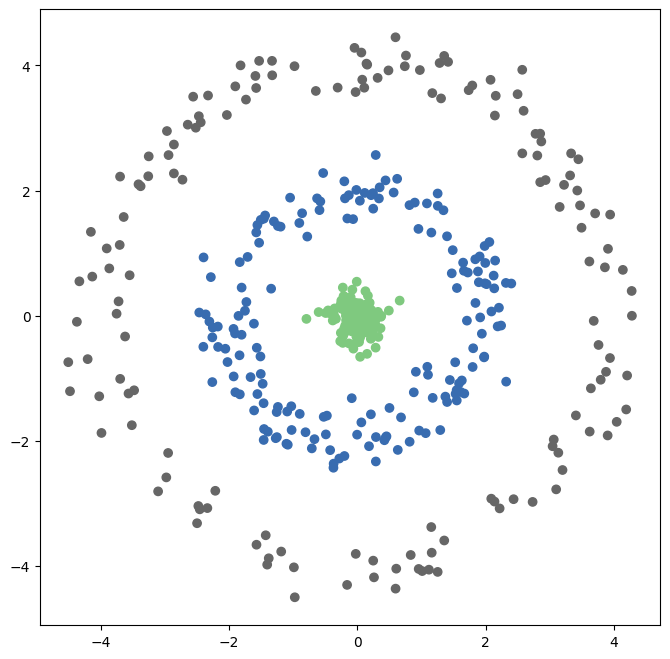
\includegraphics[width=0.5\textwidth]{601-6-1-1.png}
\caption{}
\label{601-6-1-1}
\end{figure}

PCA finds the principal linear directions of the data, i.e., directions that linearly separate the data. For this concentric data, where there are no dominant directions, PCA fails to separate the classes. 

Therefore, we project the data onto a higher dimensional space in which the data is sparse and easily separated, then we work on the projection.

\subsection{PCA with basis expansion}

\textbf{Example 6.1.1}
For data point $y = (y_1, y_2)\in \R^2$, use the mapping 
\[\phi(y) = (y_1,y_2,y_1^2,y_2^2)\in\R^4\]
The idea is to induce the linear method PCA to pick up the
representation $y_1^2+y_2^2$, which is the square of the distance from the origin.\\

Run PCA on the data expanded with $\phi$ given above and plot the first two principal components.

\begin{figure}[h]
\centering
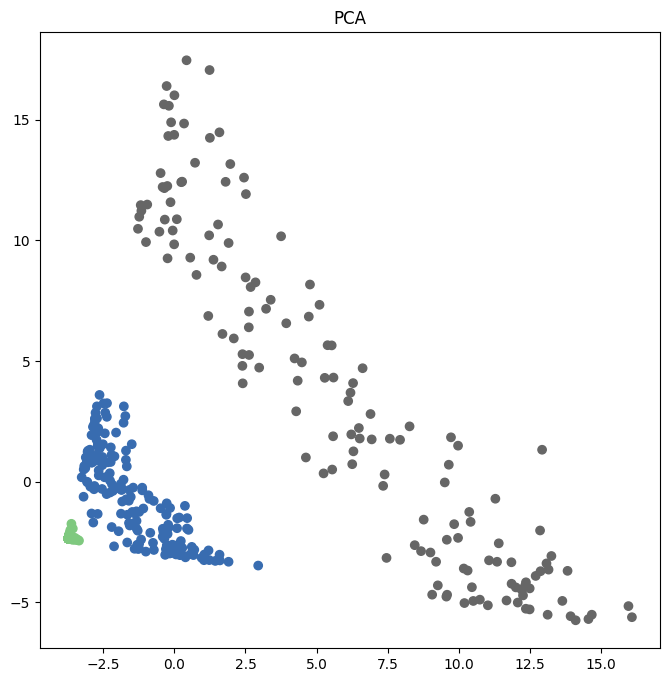
\includegraphics[width=0.5\textwidth]{601-6-1-2.png}
\caption{Result for PCA with basis expansion}
\label{601-6-1-2}
\end{figure}

\paragraph{Idea} Map the data $y = (y_1, y_2)\in \R^q$ to a more complicated space via a nonlinear mapping $\phi: \;\R^q \rightarrow\R^M$. \\
Let $\Phi \in \R^{n\times M}$ be expanded data, we then apply regular PCA to reduce the dimensionality to get a good representation of the data, which computes the SVD of the covariance $\frac1n \Phi^T\Phi \in \R^{M\times M}$.\\
$\phi(y_i)$ is a $M$-dim vector.

\textbf{Note: } this is computationally expensive for large $M$.\\



Suppose that you have an "oracle" that computes $K(y,y') = \langle\phi(y),\phi(y')\rangle$ for any $y,y'\in\R^q$ \textbf{very quickly}. How to run PCA on expanded data $\Phi$ with $M\gg n$ efficiently using the oracle?\label{here}

\textcolor{brown}{
Regular PCA on $\Phi$ needs top eigenvectors of $\Phi^T\Phi_{M\times M}$:\\
\[\Phi^T\Phi v=\lambda v\]
The score is $\alpha = \Phi v \in \R^n$.
So
\[\Phi^T\Phi (\Phi^T\Phi)v=\lambda\Phi^T\Phi v\]
\[\Phi^T\Phi\Phi^T\alpha = \lambda\Phi^T\alpha\]
\[\Phi^T(\Phi\Phi^T\alpha - \lambda\alpha) = 0\]
Let $K_{n\times n} = \Phi\Phi^T$, we have
\[\Phi^T(K\alpha - \lambda\alpha) = 0\]
Next we will prove that this is equivalent to $K\alpha - \lambda\alpha = 0$:\\
Because
\[K\alpha = \Phi\Phi^T\alpha, \quad \lambda \alpha = \lambda \Phi v\]
We know that $K\alpha - \lambda \alpha\in col(\Phi)$;\\
From the equation above ($\Phi^T(\Phi\Phi^T\alpha - \lambda\alpha) = 0$), we know that $K\alpha - \lambda \alpha\in col(\Phi)^\perp$.\\
Therefore, $K\alpha - \lambda\alpha=0$.
}

\subsection{Kernel functions}
For performing PCA with basis expansion $\phi: \mathbb{R}^q \to \mathbb{R}^M$, we only need access to the Gram matrix:
  \[
    K = \Phi \Phi^T \;=\;
    \begin{pmatrix}
      K(y_1, y_1) & K(y_1, y_2) & \cdots & K(y_1, y_n) \\
      K(y_2, y_1) & K(y_2, y_2) & \cdots & K(y_2, y_n) \\
      \vdots       & \vdots     & \ddots & \vdots     \\
      K(y_n, y_1) & K(y_n, y_2) & \cdots & K(y_n, y_n)
    \end{pmatrix}
  \]
  where $K(y, y') = \langle \phi(y), \phi(y') \rangle$ and $\langle\cdot,\cdot\rangle$ is inner product. \\

Instead of specifying the basis expansion map $\phi$, Kernel PCA specifies which kernel $K$ to use.

\paragraph{Kernel function} $K: \; \mathcal{X} \times \mathcal{X} \rightarrow \R$, generally $\mathcal{X} \times \mathcal{X} \rightarrow\R$ where $\mathcal{X}$ is the sample space. In Kernel PCA we need to construct $K$ that is \textbf{symmetric} and \textbf{p.s.d.} (positive semidefinite).\\


\begin{notionbox}[p.s.d. Kernel]
    A function $K: \; \R^q \times \R^q \rightarrow \R$ is a p.s.d. kernel function if $\forall n\in \mathbb{N}$, $X_1, \dots, X_n\in \mathcal{X}$ and $a_1,\dots, a_n\in \R$, the matrix $K$ obtained by $K_{ij} = K(X_i,X_j)$ is symmetric and $a^TKa \ge 0$.
\end{notionbox}



\textbf{Mercer's Theorem}
For any p.s.d. kernel $K$, there exists a feature map $\Phi$ which induces a Gram matrix given by $K$. In particular, $K$ introduces a space of functions generated by the linear space of $\{K(\cdot, y), \forall y \in \R^q\} = \mathcal{H}_K$ with the inner product $\langle K(\cdot,y),K(x,\cdot)\rangle = K(x,y)$, where $\mathcal{H}_K$ represents a RKHS which will be introduced in the next section.\\
\\

To simplify, for any p.s.d. $K$, there exists a map
\[\phi: \R^q \rightarrow \mathcal{H}_K\]
\[y\rightarrow \phi(y)\]
where $K(x,y) = \langle \phi(x), \phi(y) \rangle$.\\
\\

\textbf{examples:}
\begin{enumerate}
    \item \textbf{Linear PCA}:\\
    $x,y \in \R^q$, we have 
    \[K(x,y) = x^Ty,\quad \phi(x) = x, \quad \mathcal{H}_K = \R^q\]
    \item \textbf{Polynomial kernel}:\\
    $x,y \in \R^q$, we have
    \[K(x,y) = (1+x^Ty)^d\]
    Particularly, if $q = 2$, $x,y \in \R^2$, then
    \[K(x,y) = (1+x^Ty)^2 = 1+2x_1y_1+2x_2y_2+x_1^2y_1^2+x_2^2y_2^2+2x_1x_2y_1y_2 = \phi(x)\phi(y)\]
    where $\phi(x) = (1, \sqrt{2}x_1, \sqrt{2}x_2, x_1^2,x_2^2, \sqrt{2}x_1x_2)^T \in \R^6$, $\phi:\;\R^2\rightarrow\R^6$ and $\phi(x)\in\mathcal{K} = \R^6$.\\
    However, $\Phi$ does not often have closed forms.
    \item \textbf{Gaussian kernel (a.k.a. RBF kernel)}:\\
    $x,y \in \R^q$, we have 
    \[K(x,y) = \exp\{-\frac{1}{\sigma^2}\|x-y\|_2^2\}\]
    where $\sigma^2$ is a user-specified scaling parameter.\\
    Here $\phi(x)$ is infinite-dimension and has no closed-form expression. One can use the Taylor expansion to prove this fact.
    \textcolor{blue}{
    \begin{proof}[Proof sketch]
        \[K(x,y) = \exp\{-\frac{1}{\sigma^2}\|x-y\|_2^2\}\]
        \[ = \exp\{-\frac{1}{\sigma^2}\|x\|_2^2\}\exp\{-\frac{1}{\sigma^2}\|y\|_2^2\}\exp\{-\frac{2}{\sigma^2}x^Ty\}\]
        \[= c(x)c(y)\sum_{k=0}^{\infty}\frac{(x^Ty)^k}{k!}\; (Taylor\;Expansion)\]
        \[ = \sum_{k=0}^{\infty}c\cdot\langle \frac{1}{\sqrt{k!}} c(x)x^k,\frac{1}{\sqrt{k!}} c(y)y^k\rangle\]
    \end{proof}
    }
\end{enumerate}

\subsection{Kernel PCA method}
Kernel PCA can be viewed as doing PCA with possibly infinite-dimensional feature mapping $\phi$.
There are two methods for Kernel PCA.
\begin{enumerate}
    \item \textbf{Method 1}:\\
    If we have successfully calculated $\Phi$, then we can just calculate the principal components of $\Phi$. 
    \item \textbf{Method 2}:\\
    More often, as we mentioned before, $\Phi$ does not have closed forms, e.g., it may have infinite dimensions. Then we work on the Gram matrix $K = (\langle \phi(x_i),\phi(x_j)\rangle)_{n\times n}$.
\end{enumerate}

\begin{referencebox}
    Chapter 12, Section 3, \textit{PRML}.
\end{referencebox}


Consider the case where $\Phi$ has been centered, i.e., $\sum_{i=1}^n \phi(y_i) = 0$ and $\mathcal{H}_k$ is $m$-dim ($m\gg q$).\\

Let $C = \frac1n\sum_{i=1}^n\phi(y_i)\phi(y_i)^T$, then $C v_j = \lambda_j v_j$, $j = 1,\dots, m$ where $\lambda_j$ and $v_j$ are the eigenvalues and corresponding eigenvectors. 

\paragraph{GOAL} Solve the problem without exploring $\mathcal{H}_K$ directly because $\Phi$ can be difficult to compute.\\

From the equations above, we have
\[Cv_j = \frac1n\sum_{i=1}^n\phi(y_i)\phi(y_i)^Tv_j = \frac1n\sum_{i=1}^n\phi(y_i)\langle\phi(y_i), v_j\rangle = \lambda_j v_j\]
In other words, $v_j$ can be given by the linear combinations of $\phi(y_i)$:
\[v_j = \sum_{i=1}^n a_{ji}\phi(y_i) = \Phi^Ta_j\]
where $a_{ji}$ are some nonzero numbers.\\
Matrix notation:\\
$a_j = \begin{pmatrix}
 a_{j1}
 \\\vdots
\\a_{jn}
\end{pmatrix}$ and $\Phi_{n\times m} = \begin{pmatrix}
 \phi(y_i)^T
 \\\vdots
\\\phi(y_n)^T
\end{pmatrix}$.\\

\textbf{Note: }$a_j$ is a $n$-dim vector, and $v_j$ is a $M$-dim vector.\\

Thus, $C_{M\times M} = \frac1n\Phi^T\Phi$, so $\frac1n\Phi\Phi^T\Phi v_j = \lambda\Phi v_j$. Because $v_j =\Phi^Ta_j$, the equation becomes
\[\frac1n\Phi\Phi^T\Phi\Phi^Ta_j = \lambda \Phi\Phi^Ta_j\]
\[\frac1nK_nK_na_j = \lambda K_na_j\]

So we do not need to calculate $\Phi$ in fact. Instead, we only need $K$.

Similarly to~\ref{here}, we have \[\frac1nK_na_j = \lambda a_j\]
and the solution differs from the above equation only when $a_j$ are the eigenvectors of $\frac1nK_n$ corresponding to $\lambda_j = 0$.\\

Then we can perform eigen-decomposition on $\frac1nK_n$. $a_j$ are the eigenvectors. For $C = \frac1n\Phi^T\Phi$, its eigenvectors $v_j = \frac{1}{\sqrt{n\lambda_j}}\Phi^Ta_j$ with $\|v_j\| = 1$. 


\textbf{Note: }$\sqrt{n\lambda_j} = \|v_j\| = \sqrt{v_j^Tv_j}$ is used for standardization.

\subsection{Summary of Kernel PCA}
For data $y_1,\dots,y_n\in \R^q$, we have a kernel $K$ mapping it to $\phi(y_1), \dots, \phi(y_n)\in\mathcal{H}_K$ where $K$ is symmetric and p.s.d.\\
To compute the principal components of $\Phi$, let $C = \frac1n\sum_{i=1}^n\phi(y_i)\phi(y_i)^T$, $Cv_j = \lambda v_j$, $j = 1,\dots, M$.
Because closed form expressions for $\Phi$ are often unavailable, we work on the Gram matrix $K_{n\times n}$. \\
We perform eigen-decomposition on $\frac1nK$ and get eigenvalues $\lambda_j$ and eigenvectors $a_j$. Then we choose the top $p$ $a_j$'s and return a $n\times p$ matrix $A_p = [a_1, \dots, a_p]\in \R^{n\times p}$.\\
\\
The original principal components are given by $v_j = \frac{1}{\sqrt{n\lambda_j}}\Phi^Ta_j$.\\
However, we could not compute $v_j$ because we do not work with $\phi(\cdot)$, but we can compute the projection of data onto the lower-dimension principal components' directions:\\
For data point $y_i$, its projection on $v_j$ is given by
\[x_{ij} = \langle\phi(y_i), v_j\rangle = \langle \phi(y_i), \frac{1}{\sqrt{n\lambda_j}} \Phi^T a_j \rangle\]
\[=\frac{1}{\sqrt{n\lambda_j}}\phi(y_i)^T \Phi^T a_j\]
\[= \frac{1}{\sqrt{n\lambda_j}}K_i a_j\]
where $K_i$ is the $i$-th \textbf{row} of $K$.\\
The projection of all data on $v_j$ is
\[x_j = \frac{1}{\sqrt{n\lambda_j}}Ka_j\]

Once we find $a_j$, we can compute $j$-th scores for any given new data $y\in \R^q$ using the equation above:

\textcolor{blue}{
\[\langle \phi(y), v_j\rangle = \langle\phi(y),\Phi^T a_j\rangle\]
\[= \phi^T(y)\Phi^Ta_j = \langle\Phi\phi(y), a_j\rangle\]
\[= \langle \begin{pmatrix}
 \phi(y_1)^T\phi(y)\\
 \vdots\\
 \phi(y_n)^T\phi(y)
\end{pmatrix},a_j\rangle\]
\[ = \langle \begin{pmatrix}
 K(y_1,y)\\
 \vdots\\
 K(y_n,y)
\end{pmatrix},a_j\rangle\]
where $y_1,\dots, y_n$ are previous data and $\Phi$ is calculated by them.
}

\begin{notionbox}[Note]
    One must \textbf{center} the data before Kernel PCA!\\
    We set $\tilde{\phi}(y_i) = \phi(y_i) - \frac1n\sum_{i=1}^n\phi(y_i)$, $i = 1,\dots,n$. Then we have
    \[\widetilde{\Phi}_{n\times M} = (I - J)\Phi\]
    where $J_{n\times n} = \frac1n\mathbf{1}\mathbf{1}^T = \begin{pmatrix}  
  1 & 1 & \cdots & 1 \\  
  1 & 1 & \cdots & 1 \\  
  \vdots & \vdots & \ddots & \vdots \\  
  1 & 1 & \cdots & 1  
\end{pmatrix}$.\\
In practice, $\Phi$ is not often available, so we center $K$ instead:
Then \[\widetilde{K}_{n\times n} = \widetilde{\Phi}\widetilde{\Phi}^T = (I-J)K(I-J)\]
We should run this step before Kernel PCA each time!
\end{notionbox}

\subsection{Another view of Kernel PCA}
The first PC solves 
\[\underset{v_1\in\mathcal{H}_K}{\max}\frac1n\sum_{i=1}^n(v_1(y_i) - \bar{v})^2, \quad s.t.\; \|v_1\|_{\mathcal{H}_K} = 1\]
where $v_1(y_i) = \phi(y_i)^Tv_1 = x_{i1}$, additionally $\bar{v} = \frac1n\sum_{i=1}^nv_1(y_i) = \frac1n\sum_{i=1}^n\phi(y_i)^Tv_1 = 0$ because $\phi(y)$ has been centered before.\\
So the optimization means to find the first principal direction on which the variance of projection of the data is maximized.



\newpage
\section{Related Topics (I): Kernel Ridge Regression (KRR)}
\subsection{Review: Ridge Regression}

The model is 
\[Y = \theta^TX+W\] where the mean function is $E(Y|X) = \theta^TX$, $y\in\R$, $X\in\R^p$, $W$ is noise.\\

The estimate of $\theta$ is 
\[\hat{\theta} = \arg\underset{\theta\in\R^p}{\min}\sum_{i=1}^n(y_i - \theta^TX_i)^2+\lambda\|\theta\|_2^2\]
\[ = \arg\underset{\theta\in\R^p}{\min}(Y-X\theta)^T(Y-X\theta)+\lambda\theta^T\theta\]
\[ = (X^TX+\lambda I_p)^{-1}X^TY\]

By Woodbury identity, we have \[(X^TX+\lambda I_p)^{-1}X^TY = X^T(XX^T+\lambda I_n)^{-1}Y\]

Given a new data $x$, the prediction of response
\[\hat{Y} = \hat{\theta}^Tx = Y^T(XX^T+\lambda I_n)^{-1}Xx\]
where $XX^T$ is the Gram matrix. This suggests that the estimator of $Y$ depends on the Gram matrix. So we replace it with kernel.


\subsection{Reproducing Kernel Hilbert Space (RKHS)}
Let $\mathcal{H}$ be a Hilbert space of $\R$-valued functions on domain $\mathcal{X}$. A function $k: \mathcal{X}\times \mathcal{X} \rightarrow\R$ is a reproducing kernel of $\mathcal{H}$, and $\mathcal{H}$ is a \textbf{reproducing kernel Hilbert space} if 
\begin{itemize}
    \item $\forall x\in\mathcal{X}, k(\cdot, x)\in \mathcal{H}$;
    \item $\forall x\in\mathcal{X}, \forall f \in \mathcal{H}$, $\langle f(\cdot), k(\cdot, x)\rangle_\mathcal{H} = f(x)$.
\end{itemize}



\begin{notionbox}[Review: Hilbert Space]
\textbf{Hilbert Space} is a complete vector space equipped with an inner product $\langle \cdot, \cdot \rangle$ that follows: \\
Let $\mathcal{H}$ be a vector space, 
\begin{enumerate}
    \item \textbf{Inner product structure}: \\
    For any vectors $f,g,h \in \mathcal{H}$ and scalars $\alpha, \beta$, the inner product satisfies 
    \begin{itemize}
        \item linearity: $
\langle \alpha f + \beta g, h \rangle = \alpha \langle f, h \rangle + \beta \langle g, h \rangle$;
        \item symmetry: $
\langle f, g \rangle = \langle g, f \rangle$;
        \item positivity: $
\langle f, f \rangle \geq 0, \quad \langle f, f \rangle = 0 \iff f = 0$.
    \end{itemize}
    \item \textbf{completeness}: \\
    Every Cauchy sequence in $\mathcal{H}$ converges to an element within $\mathcal{H}$.\\
\end{enumerate}

\textbf{Note}: Hilbert space is more than a finite-dimension vector space. It can be an infinite-dimension function space. \\e.g., the $L^2$ space: \[
L^2(\mathbb{R}) = \left\{ f: \mathbb{R} \to \mathbb{R} \mid \int_{-\infty}^{\infty} |f(x)|^2 dx < \infty \right\}
\] where $
\langle f, g \rangle = \int_{-\infty}^{\infty} f(x) g(x) dx$.\\
\\
For RKHS, the elements in a RKHS are functions induced by kernel $k(\cdot, \cdot)$. They can be represented by the linear combination of kernel functions.

\end{notionbox}

In particular, for any $x,y \in \mathcal{X}$, 
\[k(x,y) = \langle k(\cdot, x),k(\cdot,y)\rangle_\mathcal{H}\]


\subsection{Representer Theorem}
Let function $f\in \mathcal{H}_K$ with kernel $K$. Consider
\[\hat{f} = \arg\underset{f\in\mathcal{H}_K}{\min}\sum_{i=1}^nL(y_i,  f(X_i))+\lambda\|f\|_{\mathcal{H}_K}^2\]
where $L$ is a loss function and $\|\cdot\|_{\mathcal{H}_K}$ is a norm induced by RKHS. The solution to this optimization problem may have infinite dimensions.\\

However, according to the Representer theorem, the solution to this problem must have a finite-dimension form: 
\[\hat{f}(x) = \sum_{i=1}^n\alpha_iK(x, X_i)\]
and
\[\|f\|_{\mathcal{H}_K}^2 = \alpha^TK\alpha\]
where $x, X_i \in \R^p$, $\alpha_i\in\R$.\\

This allows the original problem to be reduced to be a finite-dimension problem:
\[\hat{\alpha} = \arg\underset{\alpha\in\R^n}{\min}\sum_{i=1}^nL(y_i, \sum_{j=1}^n\alpha_jK(X_j, X_i))+\lambda\alpha^TK\alpha\]


\textcolor{blue}{
\begin{proof}
    For a function $f\in \mathcal{H}_K$, consider the decomposition 
    \[f = f_S+f_\perp\]
    where $f_S$ is the projection onto the subspace 
    \[\{f: f(x) = \sum_{i=1}^n\alpha_iK(x, X_i), \quad \alpha_1,\dots,\alpha_n\in\R\}\]
    Then, $\langle f_S, f_\perp\rangle_{\mathcal{H}_K} = 0$ and it follows that 
    \[\|f\|_{\mathcal{H}_K}^2 = \|f_S\|_{\mathcal{H}_K}^2+\|f_\perp\|_{\mathcal{H}_K}^2\ge\|f_S\|_{\mathcal{H}_K}^2\]
    Additionally, 
    \[f(X_i) = \langle f, K(\cdot, X_i)\rangle_{\mathcal{H}_K} = \langle f_S+f_\perp, K(\cdot, X_i)\rangle_{\mathcal{H}_K}\]
    \[ = \langle f_S, K(\cdot, X_i)\rangle_{\mathcal{H}_K} = f_S(X_i)\]
    So \[L(y_i,  f(X_i)) = L(y_i,  f_S(X_i))\]
    It follows that for any $f$, 
    \[\sum_{i=1}^nL(y_i,  f(X_i))+\lambda\|f\|_{\mathcal{H}_K}^2\ge \sum_{i=1}^nL(y_i,  f_S(X_i))+\lambda\|f_S\|_{\mathcal{H}_K}^2\]
    So an optimal solution $f^*$ is in the subspace, which completes the proof.
\end{proof}
}

\subsection{Kernel Ridge Regression (KRR)}
For a regression model $y = f(X)+W$, where $f\in\mathcal{H}_K$ equipped with kernel $K$. Kernel Ridge Regression aims to solve 
\[\hat{f} = \arg\underset{f\in\mathcal{H}_K}{\min}\sum_{i=1}^n(y_i-  f(X_i))^2+\lambda\|f\|_{\mathcal{H}_K}^2\]

By representer theorem, we can restrict the search space to functions of the form \[f(x) = \sum_{i=1}^n\alpha_iK(x, X_i)\]
What is the solution for $\alpha$?\\

The problem is 
\[\arg\underset{f\in\mathcal{H}_K}{\min}\sum_{i=1}^n(y_i-  \langle f, K(\cdot,X_i)\rangle_{\mathcal{H}_K})^2+\lambda\|f\|_{\mathcal{H}_K}^2\quad s.t. \;f(x) = \sum_{i=1}^n\alpha_iK(x, X_i)\]
where we can prove that \[\langle f, K(\cdot,X_i)\rangle_{\mathcal{H}_K} = \sum_{j=1}^n\alpha_j\langle K(\cdot, X_j),K(\cdot, X_i)\rangle_{\mathcal{H}_K} = \sum_{j=1}^n\alpha_jK(X_j, X_i) = f(X_i)\]
and \[\|f\|_{\mathcal{H}_K}^2 = \langle f, f\rangle_{\mathcal{H}_K} = \sum_{i=1}^n\sum_{j=1}^n\alpha_i\alpha_jK(x_i,x_j) = \alpha^TK\alpha\]

So the problem is equivalent to 
\[\arg\underset{\alpha}{\min}\|y-K\alpha\|_2^2+\lambda\alpha^TK\alpha\]

Take derivative w.r.t. $\alpha$:\\
\[K(y-K\alpha)+\lambda K\alpha = 0\]
and we obtain \textbf{the estimate of $\alpha$:}
\[\hat{\alpha} = (K(K+\lambda I))^{-1}Ky = (K+\lambda I)^{-1}y\]




Given data $x$, we can predict the values of $y$ using KRR:
\[\hat{f} = \sum_{i=1}^n\hat{\alpha}_iK(X_i,x) = \hat{\alpha}^T\begin{pmatrix}
K(X_1,x) \\
\vdots \\
K(X_n,x)
\end{pmatrix} = y^T(K+\lambda I)^{-1}\begin{pmatrix}
K(X_1,x) \\
\vdots \\
K(X_n,x)
\end{pmatrix}\]

\newpage
\section{Related Topics (II): Nonparametric Regression}
\subsection{Smoothing Splines}
For a regression model $y = f(X)+W$, where $X\in\R^p,y \in \R$. $f(\cdot)$ unknown and $W$ is the noise.\\

\paragraph{Assumption}
$f''$ exists and $f$ is in Sobolev Space. 

\begin{notionbox}[Sobolev Space]
    A space $S$ is a Sobolev space if $S$ satisfies
    \[S= \{f|f^{(v)} \text{ is absolutely continuous for } 0\le v\le m-1 \}\]
    where $f^{(m)} \in L^2([0,1])$. 
    \[\|f\|_S^2 = \sum_{v=0}^m\int_0^1 [f^{(v)}(u)]^2du\]
\end{notionbox}

\paragraph{Estimation}
For data $(y_i,x_i)$, we aims to solve
\[\hat{f} = \arg\underset{f\in S}{\min}\sum_{i=1}^n(y_i-  f(X_i))^2+\lambda \int (f''(t))^2dt\]
where $\lambda \int (f''(t))^2dt$ is the penalty function for smoothness. \\

The solution is a natural cubic spline: 
\[f(X) = \sum_{j=1}^n\theta_jN_j(X)\]
where $\theta_1, \dots, \theta_n$ are coefficients to be estimated and 
\[\left\{\begin{matrix}N_1(X) = 1
 \\N_2(X) = X
 \\\cdots
 \\N_{k+2}(X) = d_k(X) - d_{k-1}(X)
\end{matrix}\right.\]
with $d_k(X) = \frac{(X-X_k)^3_+ - (X-X_n)^3_+}{X_n-X_k}$ where $a_+ = \max(a,0)$.\\


Therefore, the problem becomes solving
\[\arg\underset{\theta\in\R}{\min}\sum_{i=1}^n(y_i- \sum_{j=1}^n\theta_jN_j(X_i))^2+\lambda \int (f''(t))^2dt\]
\[ = \arg\underset{\theta\in\R}{\min}(Y-N\theta)^T(Y-N\theta)+\lambda \theta^TK\theta\]
where $K_{n\times n} =(K_{ij})_{n\times n} = (\int N_i''(t)N_j''(t)dt)_{n\times n}$.\\

The estimates of $\theta$ and $f$ are:
\[\hat{\theta} = (N^TN+\lambda K)^{-1}Ny\]
\[\hat{f} = \sum_{j=1}^n\hat{\theta}_jN_j(X)\]


If $X\in R^2$, it is called bivariate smoothing spline.

\begin{referencebox}
    Chapter 5 Section 4, \textit{ESL}.
\end{referencebox}



When $p$ is large (here we do not mean $p>n$, we mean $p=10, 20,\dots$), how to solve nonparametric regression?\\

\textcolor{blue}{We can use Additive models.}

\subsection{Additive Model}
Suppose the model is 
\[Y = \alpha+f_1(X_1)+f_2(X_2)+\dots+f_p(X_p)+W\]
where $f_1,\dots,f_p$ are unknown functions and $f_1'',\dots,f_p''$ are well defined.


\textbf{Identifiability: }\\
\[\sum_{i=1}^nf_j(X_{ij}) = 0,\quad \forall j = 1,\dots,p\]
Besides, $X$ needs to be full rank so that $f_j$ can be estimated.

We need to estimate $\alpha, f_j$ by solving 
\[\arg\underset{\alpha, f_j}{\min}\sum_{i=1}^n(y_i-\alpha- \sum_{j=1}^pf_j(X_j))^2+\sum_{j=1}^p\lambda_j \int (f_j''(t))^2dt\]
where $\lambda_j$'s are smoothness tuning parameters.\\

We use backfitting algorithm: \\

\begin{notionbox}[Backfitting Algorithm for Additive Models]
Initialize $\hat{\alpha} = \bar{y}$;\\
Repeat for $j=1,\dots,p$:\\
\[\text{apply a cubic spline to } \{y_i - \hat{\alpha} - \sum_{k\ne j }\hat{f}_k(X_{ik}),\;X_{ij}\}\]
The function is $f_j = \hat{f}_j - \frac1n\sum_{i=1}^n\hat{f}_j(X_{ij})$.
\end{notionbox}


\begin{referencebox}
    Chapter 9, \textit{ESL}.
\end{referencebox}



\paragraph{Sparse Additive Model}

When $p>n$, we consider sparse additive model.\\

\begin{referencebox}
    Ravikumar, P., Lafferty, J., Liu, H., \& Wasserman, L. (2009). Sparse additive models. \textit{Journal of the Royal Statistical Society Series B: Statistical Methodology}, 71(5), 1009-1030.
\end{referencebox}
















\part{CLASSIFICATION}
\chapter{Classification}
\section{Classification Problems}
\subsection{Problem Setting}
\paragraph{Problem}
Given $(X_i, y_i),\quad i = 1,\dots,n, \quad X,y \in \mathcal{X}\times \mathcal{Y}$ where $\mathcal{Y}$ is a discrete space and $y_i$ is a class label.\\
Our \textbf{Goal} is to find a classifier $f: \; \mathcal{X} \rightarrow \mathcal{Y}$, s.t. $\hat{y} = f(X)$ is a good predictor of $y$ for a new $(X, y)$.\\

\textbf{Examples:}
\begin{itemize}
    \item Binary Classification: $y \in \{0,1\}$;
    \item Multiclass Classification: $y \in \{1,\dots, K\}$.
\end{itemize}

\paragraph{Loss function}
Loss function is used to evaluate your prediction: $l :\; \mathcal{Y}\times \mathcal{Y} \rightarrow \R$. \\

\begin{notionbox}[Example: 0-1 Loss]
\[l(y,\hat{y}) = \mathbb{I}_{(y\ne \hat{y})}\]
where $y$ is the true class label and $\hat{y}$ is the prediction. 
\end{notionbox}

When we minimize the loss function, we obtain the optimal classifier. \\
\\
Suppose $p(X,y)$ is the joint distribution of $(X,y)$. The Bayes risk of $f$ is \[R(f) = E[l(y,f(X))]\] which is called \textbf{Expected Classification Error}. e.g., we can use 0-1 loss inside, which means $R(f) = E[l(y,f(X))] = E[\mathbb{I}_{(y \ne f(X))}] = P(y \ne f(X))$. So the \textbf{Goal} is to find $f$ s.t. $R(f)$ is minimized. \\

\subsection{Classification with 0-1 Loss}
\paragraph{Binary Classification}
Consider the case when $p(X,y)$ is known. We use Binary classifier and 0-1 loss. The \textbf{optimal classifier} is $\arg\underset{k = 0,1}{\max}P(y = k|X)$. \\
\textcolor{blue}{
\[R(f) = E[l(y,f(X))] = E_X\left [ E(l(y,f(X))|X)\right]\]
\[ = E_X[l(1,f(X))P(y=1|X)+l(0,f(X))P(y=0|X)]\]
\[(\text{let } \eta(X) = P(y=1|X),)\]
\[ = E_X[\mathbb{I}_{(f(X) \ne 1)}\eta(X)+\mathbb{I}_{(f(X)\ne 0)}(1-\eta(X))]\]
\[= E_X[\mathbb{I}_{(f(X) \ne 1)}(2\eta(X)-1)+(1-\eta(X))]\]
To find $f^*$ that minimizes $R(f)$, 
\[f^* = \mathbb{I}_{(\eta(X)\ge \frac12)} = \mathbb{I}_{(P(y = 1|X)\ge \frac12)}\]
\[ = \arg\underset{k = 0,1}{\max}P(y = k|X)\] is the optimal Bayes Classifier. \\
}

This motivates us to 
\begin{enumerate}
    \item obtain good estimators of $P(y = k|X)$;
    \item set $\hat{f}(X) = \mathbb{I}_{(\hat{\eta}(X)\ge \frac12)}$.
\end{enumerate}

\textbf{Theorem}: For any $\hat{\eta} = \hat{P}(y = 1|X)$, if we use it to construct the optimal classifier $\hat{f} = \mathbb{I}_{(\hat{\eta}(X)\ge \frac12)} $, we have 
\[0\le R(\hat{f}) - R(f^*)\le 2 E_X|\eta(X) - \hat{\eta}(X)|\]
\textcolor{blue}{
\begin{proof}
Recall that for any classifier $f$, \[R(f) = E(l(y,f(X)) = E_X[\mathbb{I}_{(f(X) \ne 1)}\eta(X)+\mathbb{I}_{(f(X)\ne 0)}(1-\eta(X))]\]
Let $f^* = \mathbb{I}_{(\eta(X)\ge \frac12)}$, consider another classifier $\hat{f}$,
\[R(\hat{f})-R(f^*) =  E_X[\mathbb{I}_{(\hat{f}(X) \ne 1)}\eta(X)+\mathbb{I}_{(\hat{f}(X)\ne 0)}(1-\eta(X)) - (\mathbb{I}_{(f^*(X) \ne 1)}\eta(X)+\mathbb{I}_{(f^*(X)\ne 0)}(1-\eta(X)))]\]
\begin{itemize}
    \item If $\hat{f} = f^*$, $R(\hat{f})-R(f^*) = 0$;
    \item If $f^*(X) = 1,\; \hat{f}(X) = 0$, then $\eta(X) \ge \frac12$ and $R(\hat{f})-R(f^*) = \eta(X) - (1-\eta(X)) = 2|\eta(X) - \frac12|$;
    \item If $f^*(X) = 0,\; \hat{f}(X) = 1$, then $\eta(X) < \frac12$ and $R(\hat{f})-R(f^*) = (1-\eta(X)) - \eta(X) = 2|\eta(X) - \frac12|$.
\end{itemize}
In summary, \[R(\hat{f})-R(f^*) = 2E_X(\mathbb{I}_{(\hat{f}\ne f^*)}|\eta(X) - \frac12|)\]
when $f \ne f^*$, then $(\eta(X) - \frac12)(\hat{\eta}(X) - \frac12)\le 0$. This implies 
\[|\eta(X) - \hat{\eta}(X)| = |\eta(X) - \frac12|+|\hat{\eta}(X) - \frac12|\ge |\eta(X) - \frac12|\]
Therefore, \[R(\hat{f})-R(f^*) = 2E_X(\mathbb{I}_{(\hat{f}\ne f^*)}|\eta(X) - \frac12|)\le 2E_X(|\eta(X) - \hat{\eta}(X)|)\]
\end{proof}
}

\paragraph{General cases} When it comes to be $K$ labels instead of two, the optimal classifier is $f^* = \arg\underset{k}{\max}P(y=k|X)$.\\
\textcolor{blue}{
\begin{proof}
 \[\underset{f}{\max} 1-R(f) = E(\mathbb{I}_{(y = f(X))}) = E_X[E(\mathbb{I}_{(y = f(X))}|X )] \]\[= E_X[\sum_{y=1}^K P(y|X)\mathbb{I}_{(y=f(X))}]\]   
 \[ \le E_X[\sum_{y=1}^K \underset{k}{\max}P(y = k|X)\mathbb{I}_{(y=f(X))}]\]
 \[ = E_X[\underset{k}{\max}P(y= k|X)]\]
 and $" = "$ holds $\iff$ $f(X) = \arg\underset{k}{\max}P(y = k|X)$, which is the \textbf{optimal Bayes classifier}.
\end{proof}
}




\paragraph{Estimation of $P(y|X)$}
\begin{itemize}
    \item \textbf{Method 1:} Model-based approach: model the joint distribution $P(y,X)$ and then obtain $P(y|X)$.\\
    e.g., Linear discriminant Analysis (LDA); naive Bayes Classifier.
    \item \textbf{Method 2:} conditionally model $P(y|X)$.\\
    e.g., logistic regression.
\end{itemize}

\begin{referencebox}
    Chapter 4, \textit{ESL}.
\end{referencebox}

\newpage
\section{Linear discriminant Analysis (LDA)}
\subsection{Model}
\paragraph{Model Setting} $y \sim Bernoulli(\pi)$, $\pi = P(y = 1)$, $X \in \R^p$. $X|y = k \sim N_p(\mu_k, \Sigma)$, $k = 0,1$. Here the variance $\Sigma$ is the same for $k = 0,1$.
\[\eta(x) = P(y=1|X=x) = \frac{P(y=1)P(X=x|y=1)}{p(x)}\]
\textcolor{blue}{
\[\text{where  } p(x) = P(y=1)P(X=x|y=1)+P(y=0)P(X=x|y=0)\]}
\[ = \frac{1}{1+\frac{P(y=0)}{P(y=1)}\cdot\frac{P(X=x|y=0)}{P(X=x|y=1)}}\]\textcolor{blue}{
\[\text{where } p(y = 0) = 1-\pi, \; p(y=1) = \pi, X|y=0\sim N(\mu_0,\Sigma),\;X|y=1 \sim N(\mu_1,\Sigma)\]}
\[ = \frac{1}{1+\exp\{\log(\frac{1-\pi}{\pi}) - \frac12 (x-\mu_0)^T\Sigma^{-1}(x-\mu_0)+\frac12 (x-\mu_1)^T\Sigma^{-1}(x-\mu_1)\}}\]
\[ = \frac{1}{1+\exp\{-B^Tx-\gamma\}}\]
where $\begin{cases}B = \Sigma^{-1}(\mu_1 - \mu_0)
 \\\gamma = -\frac12(\mu_1 - \mu_0)^T\Sigma^{-1}(\mu_1+\mu_0)+\log(\frac{\pi}{1-\pi})
\end{cases}$\\
\paragraph{Optimal Bayes Classifier}
Therefore, the optimal Bayes Classifier $f^*$ for LDA is:
\[f^*(x) = \mathbb{I}_{(\eta(x)\ge \frac12)} = \mathbb{I}_{(B^Tx+\gamma\ge0)}\]


\subsection{Parameter Estimation}
We need to estimate $\pi, \mu_0,\mu_1,\Sigma$ (MLE).\\
\[L(\pi,\mu_0,\mu_1,\Sigma) = \prod_{i=1}^np(y_i)p(x_i|y_i)\]
\[ = \prod_{i=1}^n\pi^{y_i}(1-\pi)^{1-y_i}(2\pi)^{-\frac p2}|\Sigma|^{-\frac12}\exp\{-\frac12 (x_i-\mu_{y_i})^T\Sigma^{-1}(x_i-\mu_{y_i})\}\]
\[ = \prod_{i=1}^n\prod_{k=0}^1P(y_i = k)^{\mathbb{I}_{(y_i = k)}}p(x_i|y_i = k)^{\mathbb{I}_{(y_i = k)}}\]
So the MLEs are
\[\begin{cases}\hat{\pi} = \frac1n \sum_{i=1}^n \mathbb{I}_{(y_i = 1)}
 \\\hat{\mu_k} = \frac{\sum_{i=1}^n \mathbb{I}_{(y_i = k)}x_i}{\sum_{i=1}^n\mathbb{I}_{(y_i = k)}}
 \\\hat{\Sigma} = \frac1n \sum_{k=0}^1\sum_{i:y_i = k}(x_i - \hat{\mu_k})(x_i - \hat{\mu_k})^T
\end{cases}\]



\subsection{Quadratic Discriminant Analysis (QDA)}
We extend LDA to non-linear settings.
\paragraph{Model Setting}
$y \sim Bernoulli(\pi)$, $\pi = P(y = 1)$, $X \in \R^p$. $X|y = k \sim N_p(\mu_k, \Sigma_k)$, $k = 0,1$. Here the variances $\Sigma_k$ are different for $k = 0,1$ ($\Sigma_0 \ne \Sigma_1$).\\
\\
We set \[\log \frac{P(y = 1|X)}{P(y = 0|X)} = \delta_1(X) - \delta_0(X)\] where $\delta_k(X) = -\frac12\log|\Sigma_k| - \frac12(X-\mu_k)^T\Sigma_k^{-1}(X-\mu_k)+\log\pi_k$.\\
\\
\paragraph{Optimal Classifier}
The \textbf{optimal classifier} is $f^*(X)= \arg\underset{k = 0,1}{\max}\delta_k(X)$.\\


\subsection{Multiclass LDA \& QDA}
The model is 
\[\begin{cases}y \sim \text{Categorical Distribution}, P(y = k) = \pi_k
 \\X|y = k \sim N_p(\mu_k,\Sigma_k)
\end{cases}\]
\paragraph{Multiclass LDA}
$\Sigma_1 = \Sigma_2 = \dots = \Sigma$\\
\[\log \frac{P(y = k|X)}{P(y = l|X)} = \delta_k(X) - \delta_l(X) \]
where $\delta_k(X) = X^T\Sigma^{-1}\mu_k - \frac12 \mu_k^T\Sigma^{-1}\mu_k+\log\pi_k$.\\
The optimal classifier is \[f^*(X) = \arg\underset{k}{\max}\delta_k(X)\]
\textcolor{blue}{
\begin{proof}
    \[f^*(X) = \arg\underset{k}{\max} P(y = k|X) \]\[= \arg\underset{k}{\max}\frac{P(y = k)P(X|y=k)}{\sum_{j=1}^K P(y = j)P(X|y=j)}\]
    \[ = \arg\underset{k}{\max}P(y = k)P(X|y=k)\]
    \[= \arg\underset{k}{\max}\log P(y = k)+\log P(X|y=k)\]
    \[ = \arg\underset{k}{\max}\log \pi_k - \frac{1}{2}\log |\Sigma| - \frac12 (X-\mu_k)^T\Sigma^{-1}(X-\mu_k)\]
    \[ = \arg\underset{k}{\max}\log \pi_k  - \frac12 X^T\Sigma X+\mu_k^T\Sigma^{-1}X - \frac12\mu_k^T\Sigma^{-1}\mu_k\]
    \[ = \arg\underset{k}{\max}\log \pi_k + \mu_k^T\Sigma^{-1}X - \frac12\mu_k^T\Sigma^{-1}\mu_k\]
    \[ = \arg\underset{k}{\max} \delta_k(X)\]
\end{proof}
}

The classifier is linear in $\Sigma^{-1}$ because $\delta_k(X)$ is linear in $\Sigma^{-1}$. In practice, we need to estimate the parameters and use $\hat{\delta}(X)$ instead. 
\paragraph{Multiclass QDA}
$\Sigma_1 \ne \dots \ne \Sigma_k$\\
\[\log \frac{P(y = k|X)}{P(y = l|X)} = \delta_k'(X) - \delta_l'(X) \]
where $\delta_k'(X) = -\frac12\log|\Sigma_k| - \frac12(X-\mu_k)^T\Sigma_k^{-1}(X-\mu_k)+\log\pi_k$.\\
The optimal classifier is \[f^*(X) = \arg\underset{k}{\max}\delta_k'(X)\]



\newpage
\section{Applications of Classification}
\subsection{Generative Model}
\paragraph{Model}
\[\begin{cases} y \sim \text{Categorical}(\pi_1, \dots, \pi_K)
 \\X|y \sim P(X|y,\theta)
\end{cases}\]
\paragraph{Optimal Classifier}
\[f^*(X) = \arg\underset{k}{\max}P(y=k|X)\]
where \[P(y=k|X) = \frac{\pi_k P(X|y=k,\theta)}{\sum_{k=1}^K\pi_kP(X|y=k,\theta)}\]


\subsection{Naive Bayes Classifier}
\paragraph{Model}
\[y \sim \text{Categorical}(\pi), \;P(y = k) = \pi_k>0\]
\[X \sim \text{Categorical Dist (each $X_j$ has $L$ categories)}\]
"naive": $X_{p\times 1}|y = \begin{pmatrix}X_1
 \\\vdots
 \\X_p
\end{pmatrix}|y$ is conditionally independent, i.e., $X_i\perp X_j|y$ ($i\ne j$).

Therefore, 
\[X_j|y = k \sim \text{Categorical}(P_{ljk}),\; l = 1,\dots,L; \;j = 1,\dots, p;\;k = 1,\dots, K\]

\paragraph{Derive $P(y|X)$}
Next we derive the form of $P(y|X)$:
\[P(y = k|X) = \frac{\pi_kP(X|y=k)}{\sum_{k=1}^K\pi_kP(X|y=k)}\]
where $P(X|y=k) = \prod_{j=1}^pP(X_j|y=k) = \prod_{j=1}^p\prod_{l=1}^LP_{ljk}^{\mathbb{I}_{(X_j = l)}}$.\\

So \[P(y = k|X) = \frac{\exp\{\log \pi_k+\sum_{j=1}^p\sum_{l=1}^L\log P_{ljk}\mathbb{I}_{(X_j = l)}\}}{\sum_{k=1}^K\exp\{\log \pi_k+\sum_{j=1}^p\sum_{l=1}^L\log P_{ljk}\mathbb{I}_{(X_j = l)}\}}\]
\[ = \frac{\exp\{B_k^TZ\}}{\sum_{k=1}^K\exp\{B_k^TZ\}}\]
where $B_k = (\log \pi_k, \log P_{ljk})$ and $Z = (1, \mathbb{I}_{(X_j = l)})$. And the \textbf{optimal classifier} is the $k$ with the largest $P(y=k|X)$, i.e., $f^* = \arg\max_kP(y=k|X)$.\\
This is similar to K-class logistic regression problem.\\

\subsection{Logistic Regression}
\paragraph{Model}
This is a binary classification method for $K = 2$ case. There is no assumption on $X$ and we use binary response $y \in \{0,1\}$. Logistic Regression models $P(y|X)$ through log-odds
\[\log \frac{P(y = 1|X)}{P(y=0|X)} = \log \frac{P(y=1|X)}{1-P(y=1|X)} = 
\theta^TX = \theta_0+\theta_1X_1+\dots+\theta_pX_p\]
where $\theta = (\theta_0,\dots,\theta_p)^T$ and $X = (1,X_1, \dots, X_p)^T$.\\
\\
It is equivalent to \[y|X \sim Bernoulli(u(X))\]
where $u(X) = P(y=1|X) = \frac{e^{\theta^TX}}{1+e^{\theta^TX}}$.\\

\paragraph{Parameter Estimation}
Suppose we have data $(X_i,y_i),\;i = 1,\dots,n$. The likelihood function is 
\[L(\theta) = \prod_{i=1}^nP(y_i|X_i) = \prod_{i=1}^n u(X_i)^{y_i}(1-u(X_i))^{1-y_i}\]
\[l(\theta) = \log L(\theta) = \sum_{i=1}^n [y_i\log u(X_i)+(1-y_i)\log (1-u(X_i)]\]
\[ = \sum_{i=1}^n [y_i \theta^TX_i - \log (1+\exp (\theta^TX_i))]\]
where $u(X_i) = \frac{e^{\theta^TX_i}}{1+e^{\theta^TX_i}}$.
Take the derivative:\\
\[\frac{dl}{d\theta} = \sum_{i=1}^n[y_iX_i - \frac{\exp(\theta^TX_i)}{1+\exp(\theta^TX_i)}\cdot X_i]\]
\[ = \sum_{i=1}^n(y_i - u(X_i))X_i\]
which is called \textbf{score function}. \\
\\
There is no closed form solution to the score function. So we use some numerical methods, such as gradient descent method, Newton method, SGD method, etc.\\
\\
\textbf{Iterative Reweighted Least Square Algorithm (IRLS)}\\
It is a type of Newton - Raphson Algorithm. The Hessian matrix is
\[H = \frac{\partial^2 l(\theta)}{\partial \theta\partial \theta^T} = -\sum_{i=1}^n \frac{\partial u(X_i)}{\partial \theta}X_i^T\]
\[ = -\sum_{i=1}^n u(X_i)(1-u(X_i))X_iX_i^T = -X^TWX\]
where \[\begin{cases}X_{(n\times (p+1)} = \begin{pmatrix}X_1^T
 \\\vdots
 \\X_n^T
\end{pmatrix} = \begin{pmatrix}
 X_{11} & \cdots & X_{1p}\\
 \vdots &  & \vdots\\
 X_{n1} & \cdots & X_{np}
\end{pmatrix}
 \\
W = \begin{pmatrix}
 u(X_1)(1-u(X_1)) &   & \\
  & \ddots  & \\
  &   &u(X_n)(1-u(X_n))
\end{pmatrix}
\end{cases}\]
At time t, we update parameter $\theta$:\\

\[\begin{aligned}
\theta^{(t+1)} &= \theta^{(t)} - \left(H^{(t)}\right)^{-1}\nabla_\theta \ell(\theta)\big|_{\theta=\theta^{(t)}} \\
&= \theta^{(t)} + \left(X^T W^{(t)} X\right)^{-1}X^T\left(y - u^{(t)}\right)\\
y &= \begin{pmatrix}y_1 \\ \vdots \\ y_n\end{pmatrix},\quad u^{(t)}=\begin{pmatrix}u^{(t)}(X_1) \\ \vdots \\ u^{(t)}(X_n)\end{pmatrix}\\
\text{multiply by }H^{-1}H \quad&=\quad (H^{-1})^{(t)}\left[H^{(t)}\theta^{(t)}-X^T(y-u^{(t)})\right]\\
&= (H^{(t)})^{-1}\left[-X^T W^{(t)}X\theta^{(t)} - X^T(y - u^{(t)})\right]\\
&= -(H^{(t)})^{-1}X^TW^{(t)}\left[X\theta^{(t)} + (W^{(t)})^{-1}(y-u^{(t)})\right]\\
&= (X^T W^{(t)}X)^{-1}X^T W^{(t)}Z^{(t)}\\
\end{aligned}\]

where $Z^{(t)} = X\theta^{(t)} + (W^{(t)})^{-1}(y-u^{(t)})$ and it's weighted least square (WLS).\\
So $Z_i^{(t)} = X_i^T\theta^{(t)} + \epsilon_i^{(t)}$ where $\epsilon_i^{(t)}\sim N\left(0,\;\frac{1}{W(X_i)(1+W(X_i))}\right)$.

\paragraph{Penalized Logistic Regression}
Adding regularization to the objective function of Logistic regression still yields a linear classifier.\\
\\
LASSO:
\[ \frac1N\sum_{i=1}^n [y_i \theta^TX_i - \log (1+\exp (\theta^TX_i))]+\lambda\|\theta\|_1\]
Ridge: 
\[ \frac1N\sum_{i=1}^n [y_i \theta^TX_i - \log (1+\exp (\theta^TX_i))]+\lambda\|\theta\|_2^2\]


\subsection{Kernel Logistic Regression}
\paragraph{Model}
Here we do not use $\theta^TX$, instead we use non-linear function $f(X)$. \\
We specify a kernel function $K: \;\R^p\times \R^p \rightarrow \R$, $X\in \R^p$. The function $f$ satisfies
\[\begin{aligned}
    K\rightarrow\mathcal{H}_K\\f\in \mathcal{H}_K
\end{aligned}\]

The loss function is "-log likelihood + penalty function for $f$". 
\[\hat{f} = \arg\underset{f\in\mathcal{H}_K}{\min}\sum_{i=1}^n[-y_if(X_i)+\log(1+e^{f(X_i)})]+\frac{\lambda}{2}\|f\|_{\mathcal{H}_K}^2\]
\paragraph{Parameter Estimation}
By representer theorem, we know the solution $\hat{f}(x) = \sum_{i=1}^n \hat{\alpha_i}K(X_i,x)$ and $\hat{\alpha} = (\hat{\alpha}_1, \dots, \hat{\alpha}_n)^T_{n\times 1}$.\\
We know $\|f\|_{\mathcal{H}_K}^2 = \alpha^T K_n\alpha$, the questions becomes
\[\hat{\alpha} = \arg\min_{\alpha\in\mathbb{R}^n}\frac1n\sum_{i=1}^n[-y_i\alpha^T K_i+\log(1+e^{\alpha^T K_i})]+\frac{\lambda}{2}\alpha^TK_n\alpha\]
Use IRLS to solve this question. At t-step, 
\[\begin{cases}
    \alpha^{(t+1)} = (K_n^TWK_n+\lambda K_n)^{-1}K_n^TW^{(t)}Z^{(t)}\\
    Z^{(t+1)} = \hat{f}^{(t)}+(W^{(t)})^{-1}(y-u^{(t)})
\end{cases}\]
and $\hat{f}^{(t)} = K_n\alpha^{(t)}$.


\subsection{Generalized Additive Model (GAM)}
\paragraph{Model}
Binary response $y \in \{0,1\}$. Assume \[f(X) = \alpha + f_1(X_1) + \dots + f_p(X_p)\]
where $f_i(X_i)$ is unknown and smooth. \\
The Loss function is 
\[-\text{log likelihood}+\sum_{j=1}^p\lambda_j\int[f''_j(t_j)]^2dt_j\]
where we add smoothing penalty.

\paragraph{Parameter Estimation}
Here we use \textbf{Local Scoring Algorithm}:
\begin{enumerate}
    \item Initiate starting value $\hat{f_j} = 0,\;j=1,\dots, p$. $\hat{L} = \log (\frac{\bar{y}}{1-\bar{y}})$;
    \item Define $\hat{f}(X_i) = \hat{\alpha}+\sum_{j=1}^p \hat{f}_j$,
    \begin{enumerate}
        \item Construct $Z_i = \hat{f}(X_i)+ \frac{y_i - \hat{u_i}}{\hat{u}_i(1-\hat{u}_i)},\quad \hat{u}_i = \frac{e^{\hat{f}(X_i)}}{1+e^{\hat{f}(X_i)}}$;
        \item Set $\hat{w}_i = \hat{u}_i(1-\hat{u_i})$;
        \item Fit an additive model to $Z_i$'s with weights $w_i$ using backfitting algorithm;
        \item Repeat until convergence.
    \end{enumerate}
\end{enumerate}

The estimated function is given by
\[\hat{f}_1,\dots, \hat{f}_p = \arg\min \sum_{i=1}^n \hat{w}_i(Z_i - \hat{\alpha} -\sum_{j=1}^p f_j(X_{ij}))^2 + \sum_{j=1}^p \lambda_j \int [f_j''(t_j)]^2dt_j\]
where the first term, $\sum_{i=1}^n \hat{w}_i(Z_i - \hat{\alpha} -\sum_{j=1}^p f_j(X_{ij}))^2$ is weighted RSS; the second term, $\sum_{j=1}^p \lambda_j \int [f_j''(t_j)]^2dt_j$, is the smoothing penalty.

\begin{referencebox}
    Chapter 9 Section 1, \textit{ESL}.
\end{referencebox}

\subsection{Projection Pursuit Regression (PPR)}
This method involves nonparametric regression and dimension reduction.\\
\paragraph{Model}
We model $f(X)$ nonparametrically on $Z_i$'s where $Z_1,\dots, Z_m$ are new features that is linear combination of $X_1, \dots, X_p$ ($Z_m = W_m^TX$).
\[f(X) = \sum_{m=1}^M g_m(w_m^TX),\; w_m\in\R^p \text{ unknown and $g_m$ is unknown too.}\]
Then we perform regression
\[E(y|X) = f(X)\]
And the loss function is given by
\[\sum_{i=1}^n (y_i - \sum_{m=1}^Mg_m(w_m^TX_i)]^2)+\text{penalty }(g)\]

\paragraph{Parameter Estimation}
Use iterative algorithm.\\
For each $m = 1,\dots, M$,
\begin{itemize}
    \item Given $w_m$, use smoothing spline to get $g_m$;
    \item Given $g_m$, use Gradient based algorithms to estimate $w_m$.
\end{itemize}

\begin{notionbox}[Note]
    \begin{itemize}
        \item We select $M$ using cross-validation. When $M = 1$, it is the single index model;
        \item It is closely related to neural network where model where $f(X)$ is often specified to be multilayer.
    \end{itemize}
\end{notionbox} 

\begin{referencebox}
    Chapter 11 Section 2, \textit{ESL}.
\end{referencebox}







\chapter{Classification Trees}
\section{Classification And Regression Tree (CART)}

\subsection{Idea}

Partition the sample space (feature space) into hypercubes (regions) and assign classes to each hypercube (region).\\


\textbf{Example 8.1.1}\\
Suppose $X = \begin{pmatrix}
    X_1\\X_2
\end{pmatrix} \in [0,1]^2$. Construct a classification tree:\\

\begin{figure}[h]
    \begin{tikzpicture}

        \begin{scope}[scale=0.2]
            \node[draw, rectangle] (root) at (0,0) {$X_1 \leq t_1$};

            \node[draw, rectangle, below left=0.6cm and 0.75cm of root] (left) {$X_1 \leq t_2$};
            \draw (root.south) -- (left.north);
            
            \node[draw, rectangle, below left=0.6cm and 0.5cm of left] (R1) {$R_1$};
            \node[draw, rectangle, below right=0.6cm and 0.5cm of left] (R2) {$R_2$};
            \draw (left.south) -- (R1.north);
            \draw (left.south) -- (R2.north);
            
            \node[draw, rectangle, below right=0.6cm and 0.75cm of root] (right) {$X_2 \leq t_3$};
            \draw (root.south) -- (right.north);
            
            \node[draw, rectangle, below left=0.6cm and 0.5cm of right] (R3) {$R_3$};
            \node[draw, rectangle, below right=0.6cm and 0.5cm of right] (R4) {$R_4$};
            \draw (right.south) -- (R3.north);
            \draw (right.south) -- (R4.north);
        \end{scope}

        \begin{scope}[shift={(5,0)}, scale=0.6]
            \draw (0,0) rectangle (4,6);

            \draw (0,4) -- (4,4);
            \draw (0,2) -- (4,2);
            \draw (2,0) -- (2,2);

            \node at (2,5) { $R_2$ };
            \node at (2,3) { $R_3$ };
            \node at (1,1) { $R_1$ };
            \node at (3,1) { $R_4$ };

            \node[left] at (0,4) { $t_3$ };
            \node[left] at (0,2) { $t_1$ };
            \node[below] at (2,0) { $t_2$ };
        \end{scope}
    \end{tikzpicture}
\end{figure}

\begin{notionbox}[Notes]
    In this section, we only talk about classification trees. Regression trees will not be included.
\end{notionbox}

\subsection{CART}
Suppose we have data $(y_i,X_i)_{i=1}^n$ where $X_i \in \R^p,\quad y_i \in \{1,\dots,K\}$. Suppose we have a partition of $X$ space into $M$ categories $R_1, \dots, R_M$. \\
\\
Let $\hat{p}_{mk} = \frac{1}{n_m}\sum_{X_i\in R_m}\mathbb{I}_{(y_i = k)}$, and $n_m$ is the number of observations in the $m$-th region $R_m$: $n_m = \sum_{i=1}^n \mathbb{I}_{(X_i\in R_m)}$. So this is the estimate of the proportion $p_{mk} = P(y_i = k | X_i \in R_m)$.\\
For a new observation $X^*$ in $R_m$, we classify it to 
\[K(m) = \arg \max_{1\le k\le K} \hat{p}_{mk}\]

\begin{notionbox}[Notes]
    CART can be viewed as modeling:\\
    \\
    \textbf{Binary}:
    \[P(y=1|X) = \sum_{m=1}^M p_m \mathbb{I}_{(X\in R_m)}\]
    where $p_m = P(y = 1|X \in R_m)$. The formula above is equivalent to 
    \[\log \frac{P(y=1|X)}{P(y=0|X)} = f(X) = \sum_{m=1}^M \log \frac{p_m}{1-p_m}\mathbb{I}_{(X\in R_m)}\]
    \\
    \textbf{Multiclass ($k = 1,\dots,K$)}:
    \[P(y=k|X) = \sum_{m=1}^M p_{mk}\mathbb{I}_{(X\in R_m)}\]
\end{notionbox}

Our \textbf{GOAL} is to estimate $p_{mk}$, $R_m$ and $M$ then.


\subsection{Estimation}

How to do partition of $n$ data points?\\
Use node impurity to help us to partition the data points. Our goal is to make the impurity decrease most in each step.\\
\\
\paragraph{Node impurity} Let $Q_m(T)$ to be a loss function that measures node impurity. $m$ means $m$-th region and $T$ is the tree. There are three common impurity measures as follows:
\begin{enumerate}
    \item \textbf{Misclassification error}:
    \[Q_m(T) = \frac1{n_m}\sum_{X_i\in R_m} \mathbb{I}_{(y_i \ne k(m))} = 1-\hat{p}_{mk}(m) = 1 - \underset{k}{\max} \hat{p}_{mk}\]
    where $k(m) = \arg \underset{k}{\max} \hat{p}_{mk}$ and $\hat{p}_{mk}(m) = \underset{k}{\max} \hat{p}_{mk}$;
    \item \textbf{Gini index}:
    \[Q_m(T) = \sum_{k=1}^K \hat{p}_{mk}(1-\hat{p}_{mk}) = 1 - \sum_{k=1}^K \hat{p}_{mk}^2 = \sum_{k \ne k'}\hat{p}_{mk}\hat{p}_{mk'}\]
    \item \textbf{Cross entropy (or deviance)}
    \[Q_m(T) = - \sum_{k=1}^{K} \hat{p}_{mk} \log(\hat{p}_{mk})\]
    This is the negative log likelihood. 
\end{enumerate}


From Figure 8.1, we can observe that the \textbf{misclassification error} is the least sensitive to class imbalance ($p$ close to 0 or 1); \textbf{cross entropy} is very sensitive to small or large probabilities; \textbf{Gini index} is smooth and used by default in CART.

\begin{figure}
    \centering
    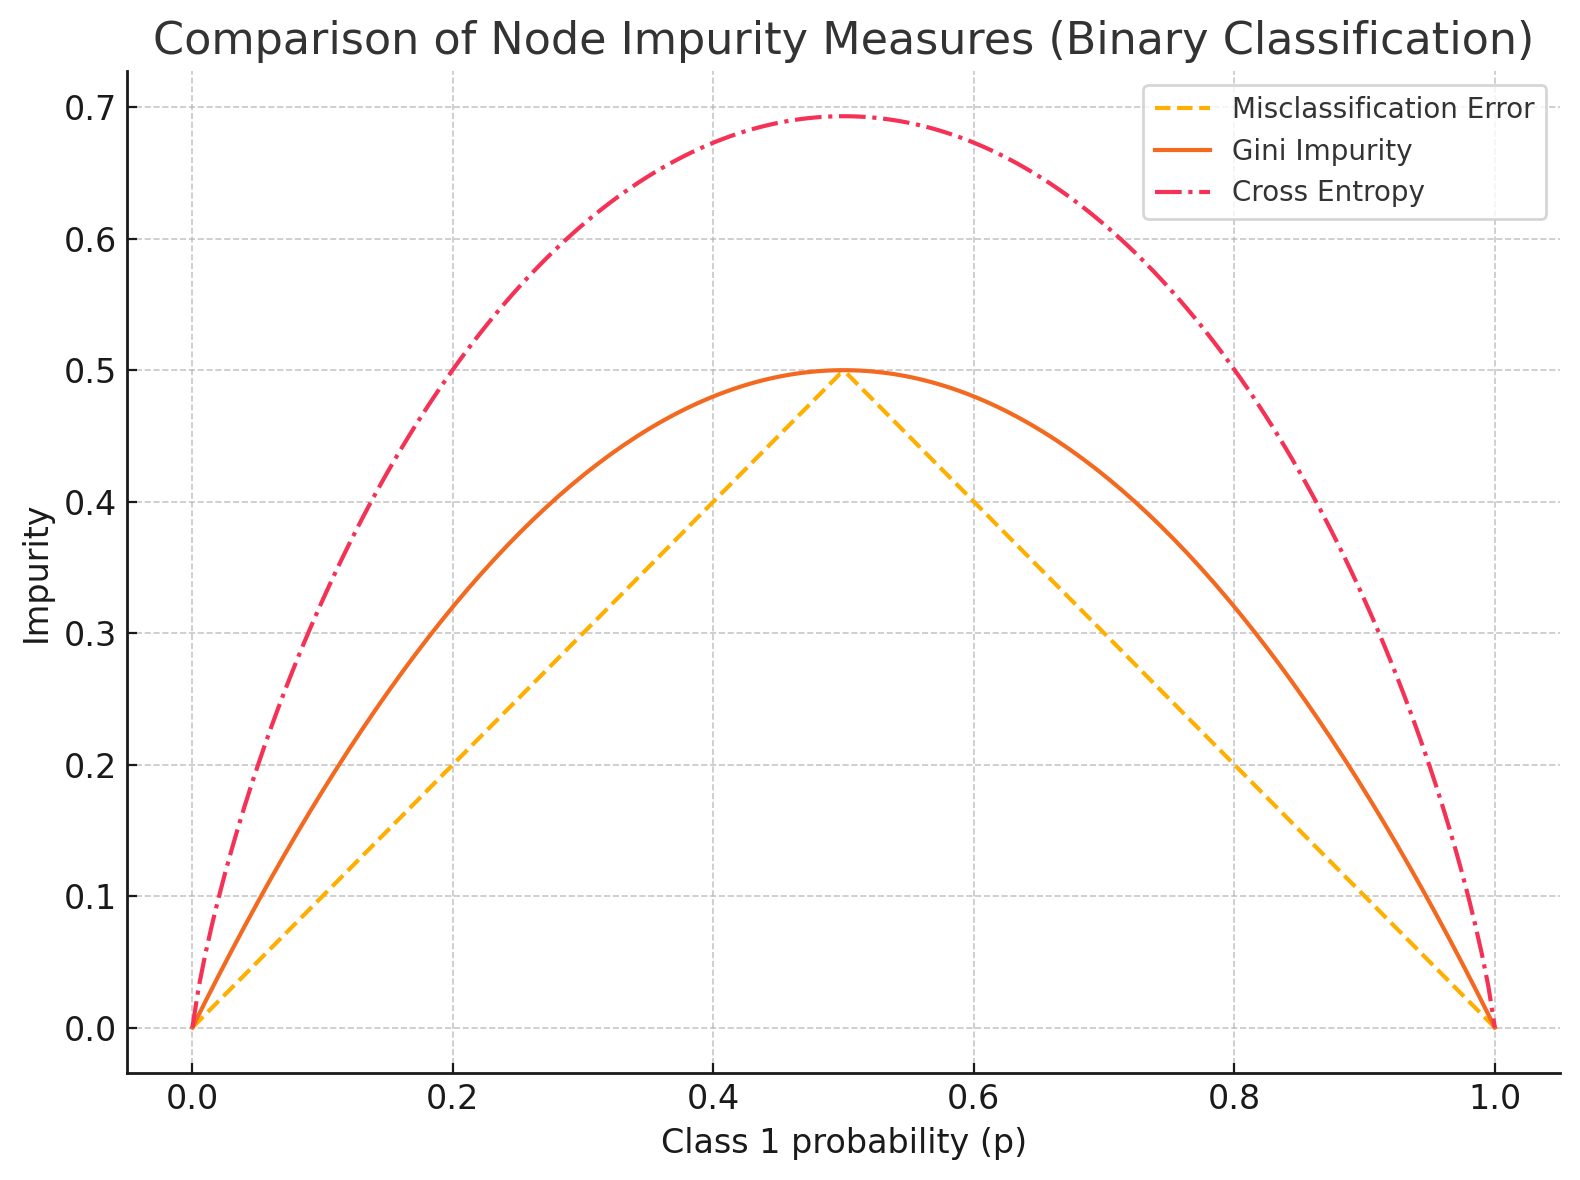
\includegraphics[width=0.5\linewidth]{601-8-1-1.png}
    \caption{comparison of three impurity measures}
    \label{601811}
\end{figure}


\paragraph{Procedure} First we start with all data points. \\
Consider a splitting variable $X_j,\; j \in \{1,\dots,p\}$ and a split point $s\in\R$. We have region 1 and region 2 
\[R_1 = \{X_j\le s\},\quad R_2 = \{X_j>s\}\]
Then estimate $j,\;s$ by \[\hat{j},\;\hat{s} = \arg\underset{j,s}{\min}(n_1Q_1+n_2Q_2)\] where $Q_1,\; Q_2$ are the loss functions for region 1 and 2; $n_1,\;n_2$ are the numbers of observations in region 1 and 2. We go through all $j$ and $s$ and choose the pair $(j,s)$ with the smallest $(n_1Q_1+n_2Q_2)$. \\
Then we do splitting and repeat the procedure inside the two subregions. \\

\paragraph{Algorithm}
First we start with a large tree $T$ (we could not split it anymore). Prune the tree by minimizing
\[C_\alpha(T) = \sum_{m=1}^{m(T)} n_mQ_m(T)+\alpha m(T)\]
where $\alpha$ is the tuning parameter which controls the number of regions. $\sum_{m=1}^{m(T)} n_mQ_m(T)$ is a kind of the total prediction error of the tree; $\alpha m(T)$ is the penalty of complexity which prevents overfitting. The more branches the tree has, the more complicated it is.


\subsection{Discussion}
Is CART a good method?\\
\\
\textbf{Advantages}: Interpretable;\\
\textbf{Disadvantages}: 
\begin{itemize}
    \item It has large variance;
    \item An error in the top split is going to affect the accuracy;
    \item Not robust.
\end{itemize}
So we use Bagging more often, which is more stable and will be introduced in the next section.



\newpage
\section{Bootstrap Aggregating (Bagging)}
\subsection{Idea}
\begin{itemize}
    \item Generate perturbed version of the data. Usually it is done by bootstrapping;
    \item Train a CART on each perturbed data;
    \item Aggregating results by majority voting.
\end{itemize}

Because trees are sensitive to small changes in data, they easily overfit. Bagging reduces model variance by averaging predictions from multiple trees trained on slightly different data, thus improving generalization.

\subsection{Procedure}
\begin{enumerate}
    \item Create $B$ bootstrapped datasets: $D_1,\dots,D_B$, where $B$ is large and $D_b$ includes $(X_i^{(b)},y^{(b)})_{i=1}^n$;
    \item Train a CART $T_b(X)$ using $D_b$ for $b = 1,\dots, B$;
    \item For a new observation, classify it to the majority class predicted by $B$ trees.
\end{enumerate}

\subsection{Discussion}
\textbf{Advantages}
\begin{itemize}
    \item Reduces the variance of CART, but does not affect the bias;
    \item It is an average of $B$ random variables;
    $T_1,\dots,T_B$ are identically distributed (not independent) with positive correlation:
    \[var (\frac{T_1+\dots+T_B}{B}) = \rho\sigma^2+\frac{1-\rho}{B}\sigma^2 \rightarrow \rho\sigma^2\quad \text{if }B \rightarrow \infty\]
    where $\rho$ represents the correlation between trees. Higher correlation means less variance reduction; lower correlation means more variance reduction.
\end{itemize}

\begin{notionbox}[Notes]
    \textbf{Compute variable (feature) importance}: the total amount that the loss function decreased by splitting over a predictor averaged over $B$ trees.\\
    \begin{itemize}
        \item Imagine you have built $B$ different trees (models) in your bagging method.
        \item For each predictor (feature), you look at every time a tree split on that predictor and measure how much that split reduced the model's loss function. 
        \item You add up all these reductions for the predictor across all $B$ trees.
        \item Finally, you average this total by dividing by the number of trees ($B$).
    \end{itemize}
\end{notionbox}



\subsection{Random Forest}
\paragraph{Procedure}
\begin{enumerate}
    \item Create $B$ bootstrapped datasets: $D_1,\dots,D_B$, where $B$ is large and $D_b$ includes $(X_i^{(b)},y^{(b)})_{i=1}^n$;
    \item Train a CART $T_b(X)$ using $D_b$ for $b = 1,\dots, B$ as follows:\\
    \textbf{at each node, consider a random subset of $(d<p)$ variables for the next split (usually $d = \sqrt{p}$ or $d<\sqrt{p}$) instead of all $p$ variables;}
    \item For a new observation, classify it to the majority class predicted by $B$ trees.
\end{enumerate}

This can increase the diversity of trees due to feature randomness. Therefore, it can further reduce variance and the risk of overfitting. 

\paragraph{Advantages}
We have $T_1,\dots,T_B$ are identically distributed (not independent) with positive correlation:
    \[var (\frac{T_1+\dots+T_B}{B})_{RF} = \rho_{RF}\sigma^2+\frac{1-\rho_{RF}}{B}\sigma^2 \rightarrow \rho_{RF}\sigma^2\quad \text{if }B \rightarrow \infty\]
    where $\rho_{RF}$ represents the correlation between trees. It is smaller than $\rho$ in Bagging because of the random subsets. Therefore, the variance of Random Forest is smaller than Bagging.

\begin{referencebox}
    Chapter 15, \textit{ESL}.
\end{referencebox}






\newpage
\section{Boosting}
Famous boosting methods: AdaBoost, Gradient Boosting (XGBoost, GBDT, LightGBM, CatBoost).
\paragraph{Main Idea} 
Boosting makes predictions by sequentially combining a sequence of weak classifiers (e.g., trees). \\Most boosting algorithms consist of iteratively learning weak classifiers w.r.t. a distribution and adding them to a final strong classifier. \\
When they are added, they are weighted in a way that is related to the weak learners’ accuracy. After a weak learner is added, the data weights are readjusted, known as ”re-weighting”. \\

\textbf{Note:}
\begin{itemize}
    \item Weak classifiers must be better than random guessing;
    \item Misclassified input data gain a higher weight and examples that are classified correctly lose weight. Thus, future weak learners focus more on the examples that previous weak learners misclassified.
\end{itemize}

\begin{referencebox}
    Chapter 10, \textit{ESL}.
\end{referencebox}
\




\subsection{Adaptive Boosting (AdaBoost)}
\paragraph{Procedure}
\begin{center}
\begin{tikzpicture}[node distance=1.5cm]
\node (start) [startstop] {We have a sample $\mathcal{D} = \{(X_i, y_i),i = 1,\dots, n\}$ where $y_i \in \{-1,1\}$};
\node (train1) [process, below of=start] {Use sample to train weak classifier $G_1(X)$ and get weighted sample};
\node (alpha) [process, below of=train1] {Use the weighted sample to train weak classifier $G_2(X)$ and update the weights};
\node (loop) [process, below of=alpha] {Repeat for $m = 1,\dots,M$};
\node (output) [process, below of=loop] {Final classification: majority vote};
\node (last) [startstop, below of=output] {Get final $\hat{G}(X) = \text{sign}\{\sum_{m=1}^M \alpha_mG_m(X)\}$};

\draw [arrow] (start) -- (train1);
\draw [arrow] (train1) -- (alpha);
\draw [arrow] (alpha) -- (loop);
\draw [arrow] (loop) -- (output);
\draw [arrow] (output) -- (last);

\end{tikzpicture}
\end{center}

where $\alpha_m$'s and $G_m$'s are the weights and trees calculated from the data ($\alpha_m$ is not the weight of sample $w_i$).

\begin{notionbox}[Notes]
    \begin{itemize}
        \item Each tree is grown using information from previous trees;
        \item Does not use bootstrapping. Instead, we fit trees on modified data of the original data;
        \item At $m$-th step, the observations that are misclassified get higher weights.
    \end{itemize}
\end{notionbox}


\paragraph{Algorithm}
\begin{enumerate}
    \item Initialize $w_i = \frac1n,\quad i=1,\dots, n$;
    \item For $m = 1,\dots, M$,\\
    fit $G_m(X)$ to training data $(X_i,y_i)$ with weights $w_i,\quad i=1,\dots,n$;
    \[err_{m} = \frac{\sum_{i=1}^n w_i \mathbb{I}_{(y_i \ne G_m(X_i))}}{\sum_{i=1}^n w_i}\]
    \[\alpha_m = \log \frac{1-err_m}{err_m}\]
    \item Update weights $w_i \leftarrow w_i \exp\{\alpha_m\mathbb{I}_{(y_i \ne G_m(X_i))}\}$ and scale the weights;
    \item Output: $\hat{G}(X) = sign \left(\sum_{m=1}^M \alpha_mG_m(X)\right)$.
\end{enumerate}



\begin{notionbox}[Interpretation of $\alpha_m$]
    The weight $\alpha_m$ tells the AdaBoost algorithm how much faith it should place in the $m$-th weak classifier.
    \begin{itemize}
        \item Large $\alpha_m$ (positive) means the classifier is better than random (significantly less than 50\% error) and thus deserves a stronger vote in the final ensemble;
        \item Small (positive) $\alpha_m$ means that while the classifier does some good, it is close to random and only worth a modest vote;
        \item Negative $\alpha_m$ means the classifier is actually doing worse than random guessing on this weighted dataset.
        Ideally, this should never happen because our weak learner should at least be better than random guessing.
    \end{itemize}
\end{notionbox}


\subsection{Boosting and Additive models}
Boosting can be seen as fitting on an additive model of the form
\[f(X) = \sum_{m=1}^M B_m b(X,\gamma_m)\]
where $B_m,\; m = 1, \dots, M$ are the coefficients for the model and $b(X, \gamma_m)$'s are the functions of $X$ with a set of parameters $\gamma_m$. \\
The \textbf{goal} is to solve this optimization problem:
\[\underset{\{B_m, \gamma_m\}_{m = 1}^M}{\min}\sum_{i=1}^NL(y_i, \sum_{m=1}^MB_mb_m\left(X_i, \gamma_m)\right)\]

\paragraph{Algorithm: Forward Stagewise Additive Modeling}
\begin{enumerate}
    \item Initialize $f_0(X) = 0$;
    \item For $m = 1$ to $M$, \\
    Compute 
    \[B_m, \gamma_m = \arg\underset{B, \gamma}{\min}\sum_{i=1}^n L(y_i, f_{m-1}(X_i)+Bb(X_i,\gamma));\]
    Set $f_m(X) = f_{m-1}(X)+B_mb(X, \gamma_m)$;
    \item Return $\hat{f}(X) = f_M(X)$.
\end{enumerate}


\paragraph{Equivalence of AdaBoost and Exponential loss}
Consider exponential loss function \[L(y, f(X)) = \exp\{-yf(X)\}\]
The optimal function is given by
\[f^*(X) = \arg\underset{f}{\min} E_{y|X}[\exp(-yf(X))] = \frac12 \log \frac{P(y=1|X)}{P(y = -1|X)}\]
So $P(y=1|X) = \frac{e^{f(X)}}{e^{f(X)}+e^{-f(X)}} = \frac 1{1+e^{-2f(X)}}$.\\
\\
We can show that AdaBoost is equivalent to the forward stagewise additive modeling algorithm with exponential loss.\\
\\
\textcolor{blue}{
For AdaBoost, the basis functions are the individual classifiers (trees) $G_m(X) \in \{-1, 1\}$. Consider forward stagewise additive modeling algorithm, we solve
\[(B_m, G_m) = \arg\underset{B,G}{\min}\sum_{i=1}^n\exp\{-y_i[f_{m-1}(X_i)+BG(X_i)]\}\]
This can be expressed as 
\[(B_m, G_m) = \arg\underset{B,G}{\min}\sum_{i=1}^nw_i^{(m)}\exp\{-y_iBG(X_i)\} \quad \quad (\star)\]
where $w_i^{(m)} = \exp (-yf_{m-1}(X_i))$ are weights applied to each observation and changeable at each iteration.\\
The solution to $(\star)$ is:\\
For any $B >0$, 
\[G_m = \arg\min \sum_{i=1}^n w_i^{(m)} \mathbb{I}_{(y_i \ne G(X_i))}\quad \quad (\star\star)\]
which is the classification tree that minimizes error rate for predicting $y_i$.\\}
\textcolor{brown}{
\begin{proof}
    Fix $B$, 
\[G_m = \arg\min_{G}\sum_{i=1}^n\exp\bigl(-y_i\bigl(f_{m-1}(X_i)+ BG(X_i)\bigr)\bigr)\]
\[= \arg\min_G\sum_{i=1}^n w_i^{(m)}\exp\bigl(-y_iBG(X_i)\bigr)\]
Recall $y_i\in\{-1,1\},\;G(X)\in\{-1,1\}$,
\[
= \arg\min_G\sum_{i=1}^n w_i^{(m)}\Bigl(\exp(-B)\underbrace{\mathbb{I}_{(y_i= G(X_i))}}_{=1 - \mathbb{I}_{(y_i\ne G(X_i))}}+\exp(B)\mathbb{I}_{(y_i\ne G(X_i))}\Bigr)
\]
\[= \arg\min_G\sum_{i=1}^n w_i^{(m)}\exp(-B)+\sum_{i=1}^n w_i^{(m)}\bigl(e^B - e^{-B}\bigr)\,\mathbb{I}_{(y_i\ne G(X_i))}\]
\[= \arg\min_G\sum_{i=1}^n w_i^{(m)}\,\mathbb{I}_{(y_i\ne G(X_i))}\]
\end{proof}
}
\textcolor{blue}{
Plug in $(\star\star)$ into $(\star)$, we get
\[\hat{B}_m = \frac12\log \frac{1-err_m}{err_m}\]
where $err_m = \frac{\sum_{i=1}^n w_i^{(m)}\mathbb{I}_{(y_i \ne G_m(X_i))}}{\sum_{i=1}^n w_i^{(m)}}$.}
\textcolor{brown}{
\begin{proof}
\[
B_m \;=\;\arg\min_{B}\sum_{i=1}^n\exp\Bigl(-y_i\bigl(G_{m-1}(X_i)+B\,G_m(X_i)\bigr)\Bigr)
\]
\[=\;\arg\min_{B}\sum_{i=1}^n w_i^{(m)}\exp\bigl(-B\,y_i\,G_m(X_i)\bigr)\]
\[=\;\arg\min_{B}\sum_{i=1}^n\exp(-B)\,\mathbb{I}_{(y_i=G_m(X_i))}
  \;+\;\exp(B)\,\mathbb{I}_{(y_i\neq G_m(X_i))}\]
\[=\;\arg\min_{B}\sum_{i=1}^n\exp(-B)\Bigl(1-\mathbb{I}_{(y_i\neq G_m(X_i))}\Bigr)\;+\;\exp(B)\,\mathbb{I}_{(y_i\neq G_m(X_i))}\]
\[=\;\arg\min_{B}\sum_{i=1}^n w_i^{(m)}\Bigl[e^{-B}+(e^{B}-e^{-B})\,\mathbb{I}_{(y_i\neq G_m(X_i))}\Bigr]\]
\[=\arg\min_{B}\;e^{-B} + (e^{B}-e^{-B})\,\mathrm{err}_m\]
where 
\[\mathrm{err}_m=\frac{\sum_{i=1}^n w_i^{(m)}\,\mathbb{I}_{(y_i\neq G_m(X_i))}}{\sum_{i=1}^n w_i^{(m)}}\]
Calculate the derivative, and we can find the best value for $B_m$ is:
\[B_m = \frac12\log \frac{1-err_m}{err_m}\]
\end{proof}
}
\textcolor{blue}{
Then $f_m(X) = f_{m-1}(X)+B_m(G_m(X))$ and $w_i^{(m)} = w_i^{(m)}\exp\{-B_my_iG_m(X_i)\}$.\\
Use the fact that \[-y_iG_m(X_i) = 2\mathbb{I}_{(y_i \ne G_m(X_i))}-1\]
We update weights by
\[w_i^{(m+1)} = w_i^{(m)} \exp\{\alpha_m\mathbb{I}_{(y_i\ne G_m(X_i))}\}\]
where $\alpha_m = 2B_m$. The steps above are the same as AdaBoost's method. 
}


\begin{referencebox}
    Friedman, J., Hastie, T., \& Tibshirani, R. (2000). Additive logistic regression: a statistical view of boosting. \textit{The annals of statistics}, 28(2), 337-407.
\end{referencebox}




\subsection{Gradient Boosting}
While AdaBoost tries to fit a tree that minimizes the loss, Gradient Boosting tries to fit the gradient, which is arguably easier. \\
\\
Here we use Steepest Descent algorithm, a.k.a. Gradient Descent Algorithm. Note that we need to find the optimal step size (or learning rate) at each step!


\paragraph{Algorithm: Gradient Tree Boosting}

\begin{enumerate}
    \item We have dataset $\displaystyle \mathcal{D} = \bigl\{(X_i, y_i)\bigr\}_{i=1}^n$, initialize $G_0(X) = \arg\min_{\gamma}\; \sum_{i=1}^n L\bigl(y_i,\gamma\bigr)$;
    \item For $m = 1,\dots,M$,
    \begin{enumerate}
        \item[\textbf{(a)}] Compute (negative) gradients:\\
        \[
        g_{im} = -\frac{\partial L\bigl(y_i,G_{m-1}(X_i)\bigr)}{\partial G_{m-1}(X_i)}.
        \]

        \item[\textbf{(b)}] Fit a tree to the targets $g_{im}$ to get terminal regions $R_{jm},\;j = 1,\dots,J_m$.

        \item[\textbf{(c)}] Compute for each terminal node:\\
        \[
        b_{jm} 
        \;=\;\arg\min_{b}\;\sum_{X_i \,\in\, R_{jm}} 
        L\Bigl(y_i,\;G_{m-1}(X_i)\;+\;b\Bigr).
        \]

        \item[\textbf{(d)}] Take the gradient step:\\
        \[
        G_m(X) 
        \;=\; G_{m-1}(X)\;+\;\sum_{j=1}^{J_m} b_{jm}\,\mathbb{I}_{(X \in R_{jm})}.
        \]
    \end{enumerate}
\end{enumerate}

\noindent
\textbf{Return:} $\displaystyle \hat{G}(X) \;=\; G_M(X).$


\begin{referencebox}
    Chapter 10, Section 10, \textit{ESL}.
\end{referencebox}


\newpage
\section{Support Vector Machine (SVM)}
\subsection{SVM}
\begin{referencebox}
    Chapter 12, \textit{ESL};\\
    Chapter 7, \textit{PRML}.
\end{referencebox}
We focus on binary classification, usually $\mathcal{Y} = \{-1,1\}$ and we observe $(X_i,y_i)_{i=1}^n$ from $p(X,y)$.

\paragraph{Assumptions}
We assume two classes can be separated by at least one hyperplane. A (linear) hyperplane can be written as $f(X) = B_0 + B^TX = 0,\quad X\in \R^p$. 

\begin{figure}[h]
\centering
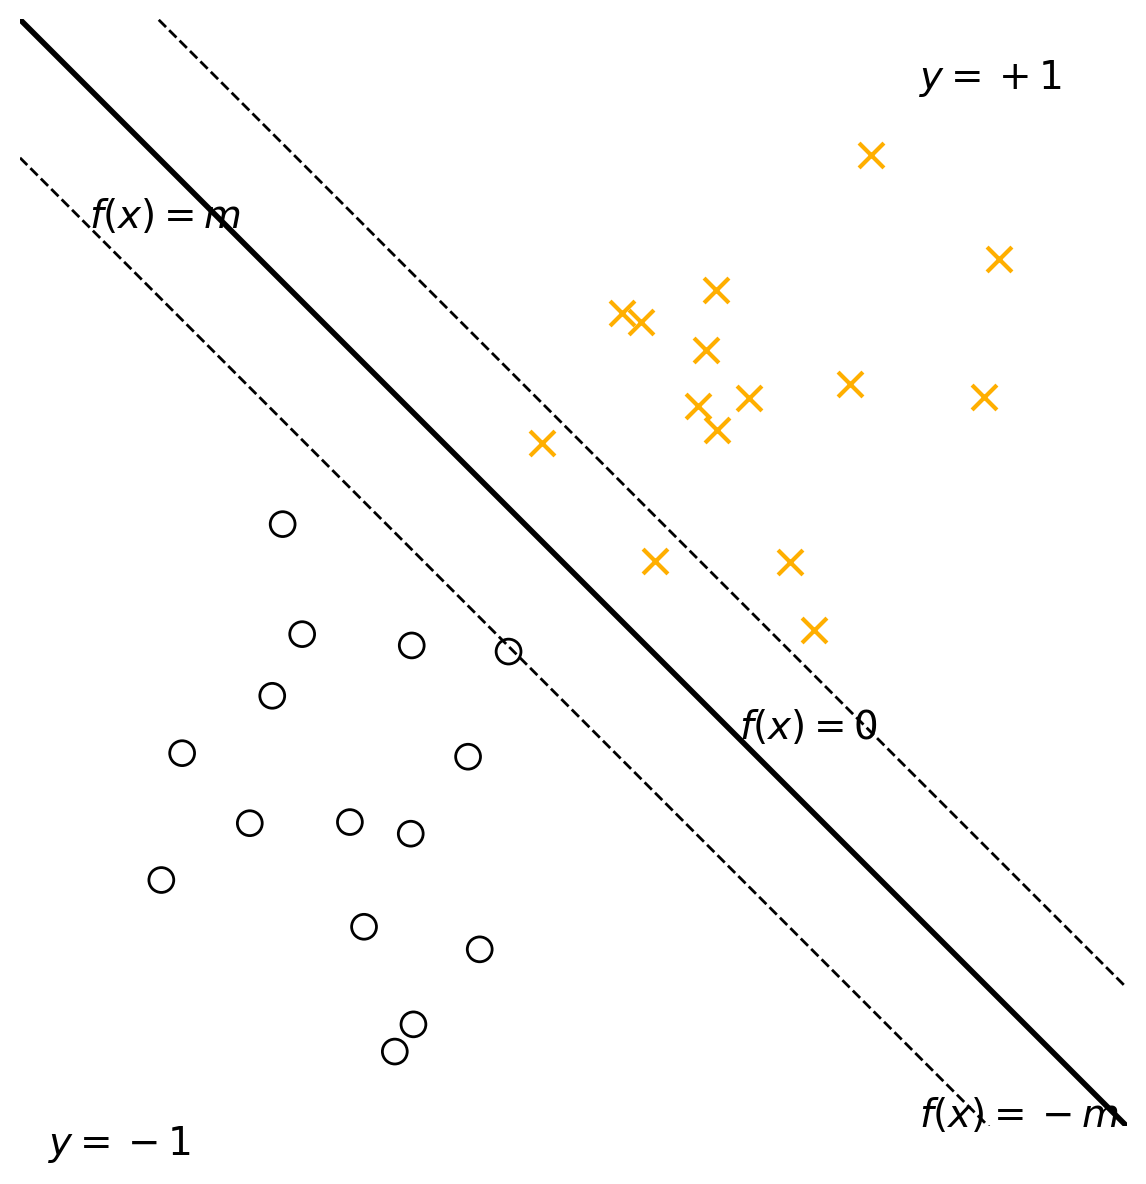
\includegraphics[width=0.5\textwidth]{601-8-4-1.png}
\caption{}
\label{601-8-4-1}
\end{figure}

Calculation rule:
\[y = \begin{cases}1 \quad\text{if } f(X) >0
 \\-1 \quad \text{if } f(X) <0
\end{cases}\]


\begin{notionbox}[Notes]
    For any points $X_1, X_2$ in $L: f(X) = 0$:
    \[\begin{cases}
        B_0+B^TX_1= 0\\
        B_0+B^TX_2 = 0
    \end{cases} \quad\Rightarrow\quad B^T(X_1 - X_2) = 0 \quad\Rightarrow\quad B\perp L\]
    Let $B^* = \frac{B}{\|B\|_2}$ be a unit vector that orthogonal to $L$. \\
    The distance of any point $X_i$ to $L$ is 
    \[\frac{f(X_i)y_i}{\|B\|_2}\]

    \textcolor{blue}{
    \begin{proof}
        Assume $y_i>0$, $\forall X_1 \in L$, we have 
        \begin{align*}
            (B^*)^T(X_i - X_1) &= \frac{1}{\|B\|_2}B^T(X_i- X_1)\\
            & = \frac1 {\|B\|_2}(B^TX_i + B_0 - 0)\\
            & = \frac1 {\|B\|_2}f(X_i)
        \end{align*}
    \end{proof}}
\end{notionbox}

\paragraph{Optimization}
SVM tries to find the best separating hyperplane that maximizes the distance from either class to the closest points.\\
The optimization problem for SVM is:
\[\max_{B_0,B}M\]
\[s.t. \quad \frac{y_i(X_i^TB+B_0)}{\|B\|_2}\ge M, \quad i=1,\dots, n\]
where $M$ represents the margin.

If we set $\|B\|_2 = \frac1M$, then it becomes 
\[\min_{B_0,B} \frac12\|B\|_2^2\]
\[s.t. \quad y_i(X_i^TB+B_0)\ge 1, \quad i=1,\dots, n\]
\textcolor{blue}{
To solve the problem, we set $\alpha_1, \dots, \alpha_n$ be the Lagrange multipliers. the Lagrangian function is 
\[L_p(B_0, B, \alpha) = \frac12 \|B\|_2^2 - \sum_{i=1}^n \alpha_i [y_i(X_i^TB+B_0)-1]\]
Take derivatives 
\[\begin{cases}
    \frac{d L_p}{dB_0} = -\sum_{i=1}^n \alpha_i y_i = 0\\
    \frac{d L_p}{dB} = B -\sum_{i=1}^n \alpha_i y_iX_i = 0
\end{cases}\]
Plug them into $L_p(B_0, B, \alpha)$, and we will get the new objective function:
\[L_D(\alpha) = \sum_{i=1}^n \alpha_i - \frac12 \sum_{i=1}^n\sum_{j=1}^n\alpha_i\alpha_jy_iy_jX_i^TX_j\]}
So the new optimization problem is 
\[\max_{\alpha}L_D(\alpha)\]
\[s.t. \begin{cases}
    \alpha_i \ge 0\\
    \sum \alpha_iy_i = 0
\end{cases}\]

\textcolor{blue}{
KKT conditions give:
\begin{itemize}
    \item $y_i(X_i^TB+B_0)\ge 1$;
    \item $\alpha_i \ge 0$;
    \item $\alpha_i[y_i(X_i^TB+B_0)-1] = 0$;
    \item $\sum \alpha_iy_i = 0, B = \sum_{i=1}^n \alpha_i y_iX_i$.
\end{itemize}
by KKT we have
\begin{itemize}
    \item If $\alpha_i > 0 $, $y_i(X_i^TB+B_0)=1$, which means $(X_i, y_i)$ are at the boundaries. They are called supported points;
    \item If $y_i(X_i^TB+B_0)>1$, then $\alpha_i = 0$.
\end{itemize}
}

Interpretation: \\
the SVM classification rule is derived by a linear combination of observation on the boundary: $$\hat{B} = \sum_{i\in S}\alpha_iy_iX_i$$ where $S$ is the set of supported points.\\
Estimation of $B_0$: $$\hat{B}_0 = \frac1 {|S|}\sum_{i\in S} (y_i - \hat{B}^TX_i)$$ because $\forall i \in S, y_i(X_i^TB+B_0) = 1$ and $y_i = \pm 1$.



\subsection{Kernel SVM}
We specify a kernel $K(X_i,X_j) \rightarrow \mathcal{H}_K$, $X_i \in \R^p \rightarrow \phi(X_i) \in \mathcal{H}_K$.\\
if $K(X_i,X_j) = X^T_iX_j$, kernel SVM reduces to linear SVM.
\paragraph{Optimization}
The optimization problem for Kernel SVM is 
\[\min_{f\ \in \mathcal{H}_K} \|f\|_{\mathcal{H}_K}\]
\[ s.t. \begin{cases}
    y_if(X_i) = y_i(X_i^TB+B_0) \ge 1, \quad i = 1,\dots,n\\
    f\in \mathcal{H}_K
\end{cases}\]

the solution can be obtained by solving 
\[\hat{\alpha} = \arg\max_{\alpha} \sum_{i=1}^n \alpha_i - \frac12\sum_{i=1}^n\sum_{j=1}^n \alpha_i\alpha_jy_iy_j K(X_i,X_j)\]
\[s.t. \;\alpha_i \ge 0, \; \sum_{i=1}^n\alpha_iy_i = 0,\quad i = 1,\dots,n\]


\subsection{Soft-margin SVM}
Consider the case when the data is not linearly separable. We maximize the margin allowing some points to be on the wrong side.

In this situation, we use slack variables $\epsilon = \begin{pmatrix} \epsilon_1
 \\\vdots
 \\\epsilon_n
\end{pmatrix}$, and the optimization problem is 
\[\min_{\epsilon, B_0,B} \frac12\|B\|_2^2\]
\[s.t.\;
\begin{cases}
    y_i(X_i^TB+B_0)\ge 1 - \epsilon_i, \quad i=1,\dots, n\\
    \epsilon_i \ge 0\\
    \sum_{i=1}^n \epsilon_i \le C
\end{cases}\]
which is equivalent to 
\[\min_{\epsilon, B_0,B} \frac12\|B\|_2^2+C\sum_{i=1}^n\epsilon_i\]
\[s.t.\;
\begin{cases}
    y_i(X_i^TB+B_0)\ge 1 - \epsilon_i, \quad i=1,\dots, n\\
    \epsilon_i \ge 0
\end{cases}\]
 where $C$ is a tuning parameter controlling the tradeoff between maximizing the margin and maximizing the training error.


Another form of the optimization problem is using Hinge loss:
\[\min_{B_0,B} \frac12\|B\|_2^2+c\sum_{i=1}^nL(y_i,f(X_i))\]
where $L(y_i, f(X_i)) = \max(1-y_if(X_i), 0)$ is Hinge loss and $f(X_i) = B_0 + B^TX_i$.






 
 
\newpage
\chapter{Special Topic: Neural Network}
\section{Shallow Neural Network}
\subsection{Data}
Suppose we have $X = \begin{pmatrix}X_1
 \\\vdots
 \\X_p
\end{pmatrix} \in \R^p$ and $y = \begin{pmatrix}y_1
 \\\vdots
 \\y_K
\end{pmatrix} \in \R^K$. If it is used for classification, then $Y = \{1,\dots, K\}$ and $y_k = \mathbb{I}_{(y=k)}$.\\

\begin{itemize}
    \item Regression: $E(y_k|x) = f_k(x)$;
    \item Classification: $p(y = k|x) = \frac{\exp[f_k(x)]}{\sum_{l=1}^K \exp[f_l(x)]}$.
\end{itemize}

\subsection{Model}
\[f_k(X) = w_{k0}^{(2)} + (w_{k}^{(2)})^TZ,\quad Z = \begin{pmatrix}Z_1
 \\\vdots
 \\Z_M
\end{pmatrix}\]
and \[Z_m = \sigma(w_{m0}^{(1)} + (w_{m}^{(1)})^TX)\]
where $w$ are model parameters: \[(w_{k}^{(2)})_{M\times1} = \begin{pmatrix}w_{k1}^{(2)}
 \\\vdots
 \\w_{kM}^{(2)}
\end{pmatrix}, \quad (w_{m}^{(1)})_{p\times1} = \begin{pmatrix}w_{m1}^{(1)}
 \\\vdots
 \\w_{mp}^{(1)}
\end{pmatrix}\]
$\sigma(\cdot)$ is an activation function.
\begin{itemize}
    \item sigmoid: $\sigma(v) = \frac{e^v}{1+e^v} = \frac1{1+e^{-v}}$;
    \item ReLU: rectified linear unit $\max(v,0)$.
\end{itemize}


\begin{center}
\begin{tikzpicture}[
  neuron/.style={circle, draw=black, minimum size=1cm},
  layer/.style={minimum height=1cm},
  >=stealth,
  shorten >=1pt, shorten <=1pt
]

\node at (0,0.5) {\color{red}Inputs};
\node[neuron] (I1) at (0,-2) {$X_1$};
\node[neuron] (Ip) at (0,-4) {$X_p$};
\node at (0,-3) {$\vdots$};

\node at (3,0.5) {\color{red}Hidden units};
\node[neuron] (H0) at (3,-0.5) {$Z_0$};
\node[neuron] (H1) at (3,-1.5) {$Z_1$};
\node[neuron] (Hm) at (3,-4.5) {$Z_m$};
\node at (3,-3) {$\vdots$};

\node at (6,0.5) {\color{red}Outputs};
\node[neuron] (O1) at (6,-2) {$Y_1$};
\node[neuron] (Ok) at (6,-4) {$Y_k$};
\node at (6,-3) {$\vdots$};

\draw[->] (I1) -- (H1) node[midway, above left] {\tiny$W_{11}^{(1)}$};
\draw[->] (I1) -- (Hm) node[midway, below left] {};
\draw[->] (Ip) -- (H1);
\draw[->] (Ip) -- (Hm);

\draw[->] (H0) -- (O1);
\draw[->] (H1) -- (O1) node[midway, above] {\tiny$W_{11}^{(2)}$};
\draw[->] (H1) -- (Ok) node[midway, above] {\tiny$W_{k1}^{(2)}$};
\draw[->] (Hm) -- (O1) node[midway, left] {\tiny$W_{1m}^{(2)}$};
\draw[->] (Hm) -- (Ok);

\node at (6,-6) {\color{red}$K$-dim};
\node at (3,-6) {\color{red}$M$-dim};
\node at (0,-6) {\color{red}$p$-dim};

\end{tikzpicture}
\end{center}

\begin{referencebox}
    Chapter 11, \textit{ESL};\\
    Chapter 5, \textit{PRML}.
\end{referencebox}






\newpage
\section{Deep Neural Network}
\subsection{Multiple hidden layers}
Suppose $Z_m^{(2)}, \quad m = 1,\dots, M_2$ is the 2nd hidden layer. We have
\[Z_m^{(2)} = \sigma(w_{m0}^{(2)} + (w_{m}^{(2)})^TZ^{(1)})\]
where $Z^{(1)}$ is the first hidden layer. 
Then, the output is denoted by 
\[f_k(x) = w_{k0}^{(3)} + (w_{k}^{(3)})_{m_2\times1}^TZ^{(2)}_{m_2\times1}\]


\begin{center}
\begin{tikzpicture}[
  neuron/.style={circle, draw=black, minimum size=1cm},
  layer/.style={minimum height=1cm},
  >=stealth,
  shorten >=1pt, shorten <=1pt
]

\node[neuron] (I1) at (0,-2) {$X_1$};
\node[neuron] (Ip) at (0,-4) {$X_p$};
\node at (0,-3) {$\vdots$};

\node at (1.5,0.5) {\color{red}1st Hidden layer};
\node[neuron] (H0) at (2,-0.5) {$Z_0^{(1)}$};
\node[neuron] (H1) at (2,-2) {$Z_1^{(1)}$};
\node[neuron] (Hm) at (2,-4.5) {$Z_m^{(1)}$};
\node at (2,-3.25) {$\vdots$};

\node at (4.5,0.5) {\color{red}2nd Hidden layer};
\node[neuron] (H0) at (4,-0.5) {$Z_0^{(2)}$};
\node[neuron] (H1) at (4,-2) {$Z_1^{(2)}$};
\node[neuron] (Hm) at (4,-4.5) {$Z_m^{(2)}$};
\node at (4,-3.25) {$\vdots$};

\node[neuron] (O1) at (6,-2) {$Y_1$};
\node[neuron] (Ok) at (6,-4) {$Y_k$};
\node at (6,-3) {$\vdots$};

\node at (6,-6) {\color{red}$K$-dim};
\node at (4,-6) {\color{red}$M_2$-dim};
\node at (2,-6) {\color{red}$M_1$-dim};
\node at (0,-6) {\color{red}$p$-dim};

\end{tikzpicture}
\end{center}

\paragraph{Why DNN works}
Since we have a lot of layers, there will be too many parameters to be estimated. \\
DNN is similar to \textbf{hierarchical interaction function class}.\\ 

Examples:
\begin{enumerate}
    \item Single index model: $f(X) = g(h(X)) = g(\theta^TX)$;
    \item Additive model: $f(X) = \sum f_l(X_l)$;
    \item Projection pursuit regression: $f(X) = \sum g_k(\theta_k^TX)$.
\end{enumerate}

\begin{referencebox}
    Kohler, M., \& Krzyżak, A. (2016). Nonparametric regression based on hierarchical interaction models. \textit{IEEE Transactions on Information Theory}, 63(3), 1620-1630.
\end{referencebox}


Function class DNN is  
\[f(X) = \mathcal{L}_{D+1} \circ \sigma \circ \mathcal{L}_D \circ \dots \circ \mathcal{L}_2 \circ \sigma \circ \mathcal{L}_1\]
where $L_j(X) = A_jX+b_j$ and $\sigma$ is the activation function.


\subsection{Convergence of DNN}
Let $f^* \in \mathcal{F}_{DNN} (p,D,W)$ be any function with the form above, where $D$ and $W$ represents depth and width; $f_0 \in H(p)$.\\

The approximation bias is given by
\[\big(\int_{[0,1]^p}|f^*(X) - f_0(X)|^2dx\big)^{\frac12}\le (DW)^{-2\gamma^*}\] where $\gamma^*$ is a constant in $H$.\\

So the estimation:
\[\|\hat{f}-\hat{f}_0\|_2 \le \sqrt{\frac1n D^2W^2\log(DW) \log n}+ (DW)^{-2\gamma^*} + \text{other bias}\]
The first term is the estimation error (variance); the second term is the approximation bias. Here there exists bias-variance tradeoff for $DW$.\\

This shows that even the depth of a neural network is 1, as long as $W$ is long enough, we will still attain convergence.\\

If we pick $DW$ approximately, 
\[\|\hat{f} - \hat{f}_0\|_2 \le (\frac{\log \sigma(n)}{n})^{\frac{\gamma^*}{2\gamma^*+1}}\]

\subsection{Estimator of the weights}
Here we only consider shallow neural network:\\
The model parameters are 
\[\left\{\begin{matrix}(w_{m0}^{(1)},w_m^{(1)})  = (w_{m0}^{(1)},\dots, w_{mp}^{(1)}),\quad m = 1,\dots, M
 \\(w_{k0}^{(2)},w_k^{(2)})  = (w_{k0}^{(2)},\dots, w_{kM}^{(2)}),\quad k = 1,\dots, K
\end{matrix}\right.\]
The loss function is 
\begin{itemize}
    \item Regression: $L(\theta) = \sum_{k=1}^K \sum_{i=1}^n[y_{ik} - f_k(X_i)]^2$;
    \item Classification: negative log lik $L(\theta) = -\sum_{k=1}^K \sum_{i=1}^ny_ik \log P(y_i = k|X)$.
\end{itemize}

We often use \textbf{Stochastic Gradient Descent (SGD)} to estimate the parameters:
\[L(\theta)=\sum_{i=1}^n L_i(\theta)\quad\text{with}\quad L_i(\theta)=\sum_{k=1}^K\bigl(y_{ik}-f_k(X_i)\bigr)^2\]

Compute partial derivatives:
\begin{align*}
\frac{\partial L_i(\theta)}{\partial w^{(2)}_{km}} 
&=\frac{\partial L_i(\theta)}{\partial f_k(X_i)}
\,\frac{\partial f_k(X_i)}{\partial w^{(2)}_{km}}\\
&=\bigl[-2\,(y_{ik}-f_k(X_i))\bigr]Z_{im},\quad
\text{where }Z_i=\begin{pmatrix}Z_{i1}\\\vdots\\Z_{i m}\end{pmatrix}.\\
\frac{\partial L_i(\theta)}{\partial w^{(1)}_{ml}}
&=\sum_{k=1}^K\frac{\partial L_i(\theta)}{\partial f_k(X_i)}
\frac{\partial f_k(X_i)}{\partial W^{(1)}_{ml}}\\
&=\sum_{k=1}^K\frac{\partial L_i(\theta)}{\partial f_k(X_i)}
\,w^{(2)}_{km}\,\sigma'\bigl(w^{(1)}_{m0}+(w^{(1)}_{m})^T X_i\bigr)\,X_{il}.\\
\end{align*}
where $\sigma'(\cdot)$ is the derivative of $\sigma(\cdot)$.

Set 
\[\delta_{ki} = -2\,(y_{ik}-f_k(X_i))\]
and 
\[S_{mi}=\sum_{k=1}^K\frac{\partial L_i(\theta)}{\partial f_k(X_i)}\,w^{(2)}_{km}\,\sigma'\bigl(w^{(1)}_{m0}+(w^{(1)}_{m})^T X_i\bigr)\]
Then \[
\begin{cases}
\displaystyle
\frac{\partial L_i(\theta)}{\partial w^{(2)}_{km}}=\delta_{ki}\,Z_{im},\\
\displaystyle
\frac{\partial L_i(\theta)}{\partial w^{(1)}_{m\ell}}=S_{mi}\,X_{il}.
\end{cases}\]

At $(t+1)$ step, 
\begin{align*}
w^{(2),\,t+1}_{km}
&= w^{(2),\,t}_{km}
- e^{(t)}[\frac{\partial L_{i_{t}}(\theta)}{\partial w^{(2)}_{km}}
-2\lambda\,w^{(2),\,t}_{km}]\\
w^{(1),\,t+1}_{ml}
&= w^{(1),\,t}_{ml}
- e^{(t)}[\frac{\partial L_{i_{t}}(\theta)}{\partial w^{(1)}_{ml}}
-2\lambda\,w^{(1),\,t}_{ml}]
\end{align*}
where $i_{i_{t}}$ are chosen randomly; $-2\lambda\,w^{(2),\,t}_{km}$ and $-2\lambda\,w^{(1),\,t}_{ml}$ are the L2 penalty, and $e$ is step size.











\newpage
\part{CLUSTERING}
\chapter{Clustering}
\section{Introduction}
\paragraph{GOAL} To group a collection of objects $X_i,\;i = 1,\dots, n$ into clusters.
\paragraph{Assumption} We assume each cluster represents a subpopulation within a heterogeneous population.\\

Different from classification, cluster labels are unknown, which is a typical feature of unsupervised learning. The clusters $Z_i \in \{1,\dots,K\}$ records the cluster membership of $i$-th observation, where $K$ is the number of clusters.


\paragraph{Clustering methods}
\begin{itemize}
    \item Data-driven approach: K-means, hierarchical clustering, spectral clustering, DBSCAN;
    \item Model-based approach: finite mixture model, latent class model.
\end{itemize}





\newpage
\section{Data-driven Clustering}
Similarity measure between $X_i$:
\begin{itemize}
    \item $D(X_i,X_j) = \|X_i - X_j\|_2$: Euclidean Distance;
    \item $D(X_i,X_j) = \sum_{l=1}^qw_ld_l(X_i,X_j)$;
    \item $\dots$
\end{itemize}

Usually we want to minimize the loss function \[W(Z) = \frac12\sum_{k=1}^K\frac1{n_k} \sum_{i:Z_i = k}\sum_{j:Z_j=k}D^2(X_i,X_j)\]
where $Z = \begin{pmatrix}
    Z_1\\\vdots\\Z_n
\end{pmatrix}$, $n_K = \sum_{i=1}^n \mathbb{I}_{(Z_i = k)}$.


\subsection{K-means}
\paragraph{Measures}
We use Euclidean Distance $D(X_i,X_j) = \|X_i - X_j\|_2$. \\
The \textbf{within cluster sum of square error (WSS)} is given by
\begin{align*}
    W(Z) &= \frac12 \sum_{k=1}^K \frac1{n_k}\sum_{i:Z_i = k}\sum_{j:Z_j=k}\|X_i - X_j\|_2^2\\
    &= \sum_{k=1}^K \sum_{i:Z_i = k} \|X_i - \mu_k\|_2^2
\end{align*}
where $\sum_{i:Z_i = k} \|X_i - \mu_k\|_2^2$ describes the variance measure for observations in the $k$-th cluster, $\mu_k = \frac1{n_k} \sum_{i:Z_i = k}X_i$ is the cluster mean of cluster $k$.\\
The \textbf{between cluster sum of square error (BSS)} is given by
\[B(Z) = \sum_{k=1}^K n_k\|\mu_k - \bar{X}\|_2^2\]
The \textbf{total sum of square error (TSS)} is
\[T = \sum_{i=1}^n \|X_i-\bar{X}\|_2^2 = W(Z) + B(Z)\] or \[TSS = WSS + BSS\]

\paragraph{Optimization}
Our goal is to minimize within cluster $W(Z)$: 
\[\min_{Z} W(Z) \Leftrightarrow\min_{Z}\sum_{k=1}^K\sum_{i:Z_i = k}\|X_i - \mu_k\|_2^2\]
which is not convex because of $Z$. Therefore, there are many local optima.\\
What we can do is running multiple initializations randomly and choosing the solution with the lowest $W(Z)$ value, e.g., $n = 10$ times.


\paragraph{Algorithm}
\begin{enumerate}
    \item Initialize means $\mu_k$, k = 1,\dots, K;
    \item Repeat until convergence:
    \begin{itemize}
        \item For $i = 1,\dots, n$, $Z_i = \arg\min_{1\le k \le K}\|X_i - \hat{\mu}_k\|_2^2$;
        \item For $k = 1,\dots, K$, $\hat{\mu}_k = \frac{\sum_{i=1}^n \mathbb{I}_{(Z_i = k)} X_i}{\sum_{i=1}^n\mathbb{I}_{(Z_i = k)}}$.
    \end{itemize}
\end{enumerate}

\paragraph{Selection of number of clusters $K$}
There are many methods for selection of $K$. Here we introduce two main methods.
\begin{enumerate}
    \item \textbf{Elbow method}\\
    We can plot $W_K(Z) - W_{K+1}(Z)$ against $K$. \\
    
    As $K$ increases, $W_K(Z)$ will decrease and decrease and the rate of decrease gradually slows down. Consequently, $W_K(Z) - W_{K+1}(Z)$will also gradually decrease and converge to 0. \\
    
    We choose the first $K$ where the decreasing trend of $W_K(Z) - W_{K+1}(Z)$ approaches 0.
    \begin{figure}[h]
\centering
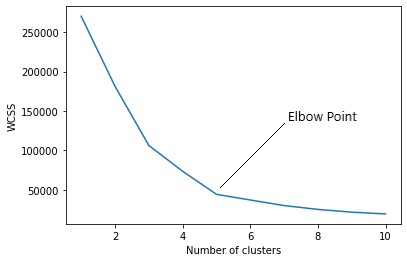
\includegraphics[width=0.5\textwidth]{601-10-2-1.png}
\caption{}
\label{601-10-2-1}
\end{figure}
    \item \textbf{Gap statistic} (proposed by Tibshirani in 2001)\\
    The procedure of selecting $K$ using Gap statistic is as follows:
\begin{itemize}
    \item For all possible $K$ values, e.g., $K = 1,\dots, K_{\max}$, run K-means and get all the $W_K(Z)$;
    \item Generate $B$ reference datasets from the original data;
    \item For each reference datasets $b = 1,\dots,B$, cluster it with $K$ clusters and get $W_K(Z)^{b*}$;
    \item Then we calculate log mean of $W_K^{b*}$:
    \[E(\log(W(Z)^*) = \frac{1}{B}\sum_{b=1}^B \log W_K(Z)^{b*}\]
    \item Calculate the Gap statistic for each $K$:
    \[Gap(K) = E(\log W_K(Z)^*) - \log W_K(Z)\]
    \item Estimate the standard deviation of $E(\log W_K(Z)^*)$:
    \[s_K' = s_K\sqrt{1+\frac1B}\]
    where \[s_K = \sqrt{\frac1B\sum_{b=1}^B[\log(W_K^{b*}) -E(\log W_K(Z)^*)]^2}\]
    \item We choose the optimal $K$ as the smallest value such that 
    \[Gap(K) \ge Gap(K+1) - s_{K+1}'\]
\end{itemize}
\end{enumerate}



\begin{referencebox}
    Tibshirani, R., Walther, G., \& Hastie, T. (2001). Estimating the number of clusters in a data set via the gap statistic. \textit{Journal of the royal statistical society: series b (statistical methodology)}, 63(2), 411-423.
\end{referencebox}



\paragraph{Non-linear K-means (Kernel K-means)}
Kernel function:
\[K(X_i,X_j)\]
\[X_i \overset{K}{\rightarrow} \phi(X_i) \in \mathcal{H}_K\]
and we perform K-means on $\phi(X)$.\\

The optimization for Kernel K-means is
\[Z = \arg\min_{Z}\sum_{k=1}^K \sum_{i:Z_i = k}\|\phi(X_i) - \mu_k\|^2_{\mathcal{H}_K}\]
which is equivalent to 
\[Z = \arg\min_{Z} \sum_{k=1}^K \sum_{i=1}^n \mathbb{I}_{(Z_i = k)}\bigl[ K(X_i,X_i) - \frac2{n_k} \sum_{j=1}^n\mathbb{I}_{(Z_j = k)} K(X_i,X_j)\]\[+\frac1{n_k^2}\sum_{j=1}^n\sum_{l=1}^n\mathbb{I}_{(Z_j = k,Z_l = k)}K(X_j,X_l)\bigr]\]


\subsection{Hierarchical Clustering}
In this method, we don't need to specify the number of clusters $K$.
\paragraph{Main idea}
Build a hierarchical representation of clusters, reflecting different levels of closeness between data points or groups. This is done by progressively merging or splitting clusters to form a tree structure (a dendrogram).

\begin{figure}[h]
\centering
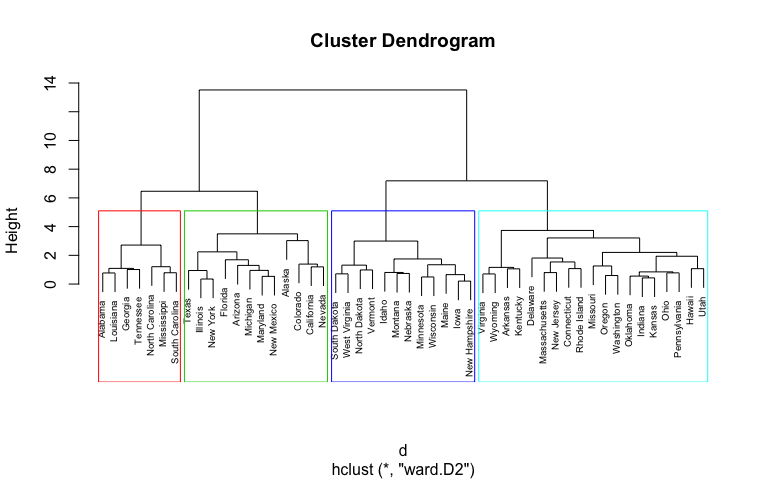
\includegraphics[width=0.75\textwidth]{601-10-2-2.png}
\caption{}
\label{601-10-2-2}
\end{figure}

\paragraph{Methods}
There are two methods for hierarchical clustering:
\begin{itemize}
    \item \textbf{Bottom-up method (Agglomerative method)}: \\
    We start with $n$ clusters for $n$ points, and then merge the two closest clusters at each step until only one cluster containing all data points remains;
    \item \textbf{Top-down method (Divisive method)}:\\
    Starts with all data points in a single cluster. At each step, it splits a cluster into two or more smaller clusters. This process is repeated until each data point forms its own individual cluster.
\end{itemize}


We use Bottom-up HC more often because of its lower time complexity.

\paragraph{Bottom up HC}
The optimization problem for this method is 
\[\min_{\mu}\frac12\sum_{i=1}^n\|X_i - \mu_i\|_2^2+\lambda\sum_{i<j} \mathbb{I}_{(\mu_i \ne \mu_j)}\]
where the cluster mean $\mu = \begin{pmatrix}
    \mu_1\\\vdots\\\mu_n
\end{pmatrix}$.\\

The problem is non-convex because of $\mathbb{I}_{(\mu_i \ne \mu_j)}$. We can modify the problem to make it convex:
\[\min_{\mu}\frac12\sum_{i=1}^n\|X_i - \mu_i\|_2^2+\lambda\sum_{i<j} \|\mu_i - \mu_j\|_q\]

When $q = 1$, it is a fused LASSO penalty; when $q=2$, it is a group fused LASSO penalty.

\begin{referencebox}
    Hocking, T. D., Joulin, A., Bach, F., \& Vert, J. P. (2011, June). Clusterpath an algorithm for clustering using convex fusion penalties. \textit{In 28th international conference on machine learning} (p. 1).
\end{referencebox}

\subsection{Biclustering}
This method can perform clustering on both rows and columns of a data matrix simultaneously, whereas common clustering methods typically only cluster rows by finding similar rows across all columns or only cluster columns.

\paragraph{Example} 
Imagine a data table where rows represent objects (e.g., genes) and columns represent features or conditions (e.g., experimental conditions).\\
\begin{itemize}
    \item Traditional row clustering finds groups of genes that behave similarly across all experimental conditions;
    \item Traditional column clustering finds groups of experimental conditions where all genes show similar behavior.
\end{itemize}

In contrast, biclustering finds a group of genes that exhibit a similar pattern only under a specific set of experimental conditions (for example, these genes are all highly expressed or show an increasing trend under these conditions).

\paragraph{Model}
Suppose we have data matrix \[X: \; X_{ij} \sim \mu_{kr} + \epsilon, \quad i= 1,\dots, n,\;j = 1,\dots, p,\; k = 1,\dots,K,\; r = 1,\dots, R\] where $K$, $R$ are the number of row clusters and column clusters. \\
The optimization problem is 
\[\min_{\mu} \frac12\sum_{k=1}^K\sum_{r=1}^R \sum_{i\in C_k} \sum_{j \in D_r}(X_{ij} - \mu_{kr})^2\]
and we can add a sparse penalty $\lambda\sum_{k}\sum_{r}|\mu_{kr}|$ if needed.\\

We can convert this problem into a convex clustering problem:
\[\min_{U}\frac12\|X-U\|_F^2 + \lambda_{\rm row} \sum_{i<i{\prime}}w_{ii{\prime}}\|U_{i\cdot}-U_{i{\prime}\cdot}\|_2
+\lambda_{\rm col}\sum_{j<j{\prime}}h_{jj{\prime}}\|U_{\cdot j}-U_{\cdot j{\prime}}\|_2.\]

Note that $U$ is not made of $\mu_{kr}$. Actually it has the same dimension as $X$. More details in the reference paper below.
\begin{referencebox}
    Chi, E. C., Allen, G. I., \& Baraniuk, R. G. (2017). Convex biclustering. \textit{Biometrics}, 73(1), 10-19.
\end{referencebox}

Or we can perform biclustering via sparse SVD:\\
Decompose $X = \sum_{k=1}^K d_ku_kv_k^T$ where $u_k$ and $v_k$ are sparse. The problem becomes 
\[\min_{u_k,v_k} \|X - duv^T\|_F^2 + \lambda_uP_1(u) + \lambda_vP_2(v)\]
where $\lambda_uP_1(u) + \lambda_vP_2(v)$ are sparse penalty on $u,v$.

\begin{referencebox}
    Lee, M., Shen, H., Huang, J. Z., \& Marron, J. S. (2010). Biclustering via sparse singular value decomposition. \textit{Biometrics}, 66(4), 1087-1095.
\end{referencebox}

\newpage
\section{Model-based Clustering}
\subsection{Finite Mixture Model}
We assume the data are from a mixture of distribution.

\paragraph{Model}
For each observable variable $X_{p\times 1}$ and latent variable $Z \in \{1,\dots, K\}$, we have
\[\begin{cases}
    Z \sim Categorical(\pi_{K\times 1}) \;\text{ with } \pi = \begin{pmatrix}
        \pi_1\\\vdots\\\pi_K
    \end{pmatrix};\\
    X|Z = k \sim P(X|\theta_k)
\end{cases}\]
where $\theta_k$ are unknown parameters.

\paragraph{Examples}
\begin{enumerate}
    \item Continuous type data $X\in \R^p$:\\
    Example:\\
    Take $P(X|\theta_k)$ as $N(X|\mu_k,\Sigma_k)$ where $\pi_k$ are the mixture probabilities and $\mu_k, \Sigma_k$ are unknown parameters, i.e.,
    \[X|Z = k \sim N(X|\mu_k, \Sigma_k)\]
    This gives Gaussian Mixture Model (\textbf{GMM}), which we have introduced in Chapter 4, and will discuss more specifically next. 
    \item Categorical data:\\
    Here we have $X_{p\times1} = \begin{pmatrix}
        X_1\\\vdots\\X_p
    \end{pmatrix}$ with $X_j \in \{1,\dots, M\}$. $X_1,\dots,X_p|Z = k$ are conditionally independent, and 
    \[X_j|Z=k \sim Categorical(\theta_{jkm})\]
    where $\theta_{jkm} = P(X_j = m|Z=k)$, and $\sum_{m=1}^M\theta_{jkm} = 1$.
    \item Mixed type data:\\
    Some of the $X_j$ are discrete variables, while some are continuous variables. \\
    \\
    Example: 
    \[X_i|Z=k \sim N(\mu_k,\Sigma_k),\quad i  = 1,\dots, \frac n2\]
    \[X_j|Z = k \sim Bernoulli(\theta_{jk}), \quad j = (\frac n2+1), \dots, n\]
\end{enumerate}


\paragraph{Gaussian Mixture Model (GMM)}
Suppose we have data $X_1,\dots,X_n \in \R^p$. The model is 
\[\begin{cases}
    Z \sim Categorical(\pi_{K\times 1}) \;\text{ with } \pi = \begin{pmatrix}
        \pi_1\\\vdots\\\pi_K
    \end{pmatrix};\\
    X|Z = k \sim N(\mu_k,\Sigma_k)
\end{cases}\]
and we want to estimate the parameters $\pi, \mu_k, \Sigma_k$. This can be done by EM algorithm:\\

\textbf{Procedure for EM algorithm}\\
The likelihood of observed data is 
\[L(\pi,\mu,\Sigma\mid X)
= \prod_{i=1}^n P\bigl(X_i \mid \pi,\mu,\Sigma\bigr)
= \prod_{i=1}^n \sum_{k=1}^K \pi_k \, N\bigl(X_i \mid \mu_k,\Sigma_k\bigr)\]
So the log likelihood is given by
\[
\ell(\pi,\mu,\Sigma\mid X)
= \log L(X\mid \pi,\mu,\Sigma)
= \sum_{i=1}^n \log\!\Bigl(\sum_{k=1}^K \pi_k\, N(X_i\mid\mu_k, \Sigma_k)\Bigr)
\]
The complete-data log likelihood is given by
\[
\ell_c(\pi,\mu,\Sigma \mid X,Z)
= \log \prod_{i=1}^n \prod_{k=1}^K 
  \bigl[\pi_k\,N(X_i\mid\mu_k,\Sigma_k)\bigr]^{z_i^k}
\]\[= \sum_{i=1}^n \sum_{k=1}^K z_{i}^k
  \bigl(\log\pi_k + \log N(X_i\mid\mu_k,\Sigma_k)\bigr)
\]
where $z_i^k = \mathbb{I}_{(Z_i = k)}$.\\

\textbf{E-step}: we compute $E_{Z|X,\pi^{(t)},\mu^{(t)},\Sigma^{(t)}}(\ell_C(\mu,\pi,\Sigma|X,Z))$.\\
For $i = 1,\dots, n$, $k = 1,\dots, K$, 
\[\tau_{ik}^{(t)} \equiv P(Z_i =k|X_i,\pi^{(t)},\mu^{(t)},\Sigma^{(t)}) = \frac{P(Z_i = k,X_i|\theta^{(t)})}{P(X_i|\theta^{(t)})}= 
\frac{\pi_k^{(t)}N\bigl(X_i|\mu_k^{(t)},\Sigma_k^{(t)}\bigr)}
     {\sum_{l=1}^K \pi_{l}^{(t)} N\bigl(X_i|\mu_{l}^{(t)}, \Sigma_{l}^{(t)}\bigr)}
\]

\textbf{M-step}: we maximize the expectation w.r.t. $\pi, \mu, \Sigma$.\\
For $k = 1,\dots, K$,
\[\begin{cases}
    \pi_k^{(t+1)} = \frac{1}{n}\sum_{i=1}^n \tau_{ik}^{(t)}\\
    \mu_k^{(t+1)} = \frac{\sum_{i=1}^n \tau_{ik}^{(t)}\,X_i}
       {\sum_{i=1}^n \tau_{ik}^{(t)}}\\
    \Sigma_k^{(t+1)} = \frac{\sum_{i=1}^n \tau_{ik}^{(t)}\,(X_i-\mu_k^{(t+1)})(X_i-\mu_k^{(t+1)})^T}
       {\sum_{i=1}^n \tau_{ik}^{(t)}}
\end{cases}\]

\textbf{Note}: We need data to follow Gaussian distribution!

\begin{notionbox}[Remark]
    EM \& GMM is a soft version of K-means.\\
    If we fix $\Sigma_k = \sigma^2I$, then when $\sigma^2 \rightarrow 0$, EM algorithm $\rightarrow$ K-means:
    \[\tau_{ik} = \frac{\pi_k\exp\{-\frac1{2\sigma^2}\|X_i - \mu_k\|_2^2\}}
     {\sum_{l=1}^K\pi_l\exp\{-\frac1{2\sigma^2}\|X_i - \mu_l\|_2^2\}}\]
\end{notionbox}

\subsection{Bayesian Approach}
Instead of computing MLE in GMM, we use Bayesian inference which is to infer the latent variable $Z$ by computing the posterior distribution of $\pi, \mu, \Sigma, Z$:\\

Given data $(X_1,\dots,X_n)$, we compute 
\[P(\pi_k|X) = \frac{P(\pi_k,X)}{P(X)} = \frac{P(X|\pi_k)P(\pi_k)}{P(X)}\]
and $P(\mu_k|X), P(\Sigma_k|X)$ similarly. We can use Gibbs sampling.

\paragraph{Example}
Consider the prior for $\pi$: \[\pi = \begin{pmatrix}
\pi_1\\\vdots\\\pi_K\end{pmatrix}\sim Dirichlet(\alpha_1,\dots, \alpha_K)\] 
with PDF $f(\pi) \propto \prod_{k=1}^K\pi_k^{\alpha_{k}-1}$. \\
The prior for $\mu_k$ and $\Sigma_k$ are 
\begin{itemize}
    \item $\mu_k \mid \Sigma_k \sim \mathcal{N}(\mu_{0k}, \Sigma_k / \kappa_0)$;
    \item $\Sigma_k \sim \text{Inverse-Wishart}(\nu_0, \Psi_0)$
\end{itemize}
For all $k = 1,\dots, K$, we repeat sampling $Z_i,\pi_k, \mu_k,\Sigma_k$ conditionally on other parameters sequentially. Finally we can estimate the posterior distribution from our samples.



\subsection{Overlapping Clustering}
Overlapping Clustering allows some variables to belong to more than one cluster simultaneously. One method for this purpose is using structured factor model.\\
\paragraph{Model}
Consider $X_{p\times 1} = A_{p\times K}Z_{K\times1}+E_{p\times1}$.\\
The loading matrix $A_{p\times K}$ characterizes the cluster membership of $X$. $A_{jk} \ne 0 \iff X_i $ belongs to Cluster $k$. \\
\\
Note that $A$ is only identifiable to signed permutation (matrix permutation or multiplying $\pm 1$). However, if $A$ satisfies
\[\begin{cases}
    \sum_{a=1}^K|A_{ja}|\le 1\\
    \exists \text{ at least two j}\in \{1,\dots,p\}, \;s.t.\;\forall b\ne a, \;|A_{ja}| = 1, \;|A_{jb}| = 0.
\end{cases}\]
then $A$ is identifiable.\\

More details can be found in the paper below.

\begin{referencebox}
    Bing, X., Bunea, F., Ning, Y., \& Wegkamp, M. (2020). Adaptive estimation in structured factor models with applications to overlapping clustering. \textit{Annals of Statistics}, 48(4).
\end{referencebox}






\end{document}  

